\documentclass[a4paper,11pt]{book}
\usepackage[utf8]{inputenc}
\usepackage[centertags]{amsmath}
\usepackage{amscd}
\usepackage{amsthm}
\usepackage{amssymb}
\usepackage{bm}
\usepackage{relsize}%relative size font
\usepackage{enumerate}
%\usepackage{xypic}
%\usepackage[dvips]{graphics}
%\usepackage{moreverb}
\usepackage{multicol}
\usepackage{multirow}
%\usepackage{ textcomp }%textsection
\usepackage[english,catalan]{babel}
%\usepackage{epsfig}
%\usepackage{rotating}
\usepackage{mathrsfs}%F rara
\usepackage{color}
\usepackage[table]{xcolor}
\usepackage{tikz}
\usetikzlibrary{matrix}
\usepackage[all,cmtip]{xy}%diagrames
%\usepackage{tabls} %per tenir més control sobre l'espai en les taules
\usepackage{array}
\usepackage{indentfirst} %per començar primer parragraf de seccio o capitol amb indent
\usepackage{inconsolata}
\usepackage[T1]{fontenc}
\usepackage[sc]{mathpazo}
%\usepackage[oneside,bindingoffset=1cm]{geometry}
\usepackage{AlegreyaSans}
\usepackage{anysize}%margins
\usepackage{graphicx}
\usepackage[font=footnotesize,labelfont=bf]{caption}
\usepackage{subcaption}%subfigures
%\usepackage{dsfont}
%\usepackage{mathtools}
%\usepackage{amsfonts}
%\usepackage{float}
%\usepackage{wrapfig}
%\usepackage{commath}
\usepackage{afterpage}
%\usepackage[official]{eurosym}
%\usepackage[bottom]{footmisc}%fixar notes de peu de pagina al final
\usepackage{fancyvrb}%verbatim inline
%\usepackage{upgreek}%per fer la \upvarphi
\usepackage{titlesec}   %per modificar espai chapters
\usepackage{lipsum} %dummy text
%\usepackage{lmodern}% http://ctan.org/pkg/lmodern
%\usepackage{slantsc}% http://ctan.org/pkg/slantsc
%\usepackage{setspace}
\usepackage[breaklinks, colorlinks=true, linkcolor=black, citecolor=blue, urlcolor=black]{hyperref}
\usepackage{listings}%coding with color
\usepackage{fancyhdr}
\usepackage{slashed}
\usepackage{arydshln}
\usepackage{ragged2e}
%\usepackage{cleveref}

%------------------------------------
%MARGES
%------------------------------------------------------------------------------------------------
\marginsize{2.5cm}{2.5cm}{2.0cm}{2.3cm}%{left}{right}{top}{bottom}
\setlength{\parskip}{0.3em plus 2pt} %paragraph separation
\linespread{1.1} % Palatino needs more leading (space between lines)

\addto{\captionsenglish}{\renewcommand{\bibname}{References}}

%%%%%%%%%%%%%%%%%%%%%%%%%%%%%%%%%%%%%%%%%%%%%%%%%%%%%%%%%%%%%%%%%%%%%%%%%
% theorem environments
%%%%%%%%%%%%%%%%%%%%%%%%%%%%%%%%%%%%%%%%%%%%%%%%%%%%%%%%%%%%%%%%%%%%%%%%%

\newtheorem{defn0}{Definition}[chapter]%section o chapter
\newtheorem{prop0}[defn0]{Proposition}
\newtheorem{thm0}[defn0]{Theorem}
\newtheorem{lemma0}[defn0]{Lemma}
\newtheorem{corollary0}[defn0]{Corollary}
\newtheorem{example0}[defn0]{Example}
\newtheorem{remark0}[defn0]{Remark}
\newtheorem{conjecture0}[defn0]{Conjecture}
\newtheorem*{notation0}{Notation}

%theorem without name
\newtheorem{manualtheoreminner}{}
\newenvironment{manualtheorem}[1]{%
  \renewcommand\themanualtheoreminner{#1}%
  \manualtheoreminner
}{\endmanualtheoreminner}

\newenvironment{definition}{ \begin{defn0}\rm}{\end{defn0}}
\newenvironment{proposition}{\begin{prop0}}{\end{prop0}}
\newenvironment{theorem}{\begin{thm0}}{\end{thm0}}
\newenvironment{lemma}{\begin{lemma0}}{\end{lemma0}}
\newenvironment{corollary}{\begin{corollary0}}{\end{corollary0}}
\newenvironment{example}{ \begin{example0}\rm}{\end{example0}}
\newenvironment{remark}{ \begin{remark0}\rm}{\end{remark0}}
\newenvironment{conjecture}{\begin{conjecture0}}{\end{conjecture0}}
\newenvironment{notation}{\begin{notation0}\rm}{\end{notation0}}

\newcommand{\defref}[1]{Definition~\ref{#1}}
\newcommand{\propref}[1]{Proposition~\ref{#1}}
\newcommand{\thmref}[1]{Theorem~\ref{#1}}
\newcommand{\lemref}[1]{Lemma~\ref{#1}}
\newcommand{\corref}[1]{Corollary~\ref{#1}}
\newcommand{\exref}[1]{Example~\ref{#1}}
\newcommand{\secref}[1]{Section~\ref{#1}}
\newcommand{\remref}[1]{Remark~\ref{#1}}
\newcommand{\conjref}[1]{Conjecture~\ref{#1}}
\newcommand{\notref}[1]{Notation~\ref{#1}}

\newcommand{\slfrac}[2]{\left.#1\middle/#2\right.}%fraccions amb slash
\newcommand{\abs}[1]{\left\lvert#1\right\rvert}%abs
\newcommand{\orbit}[1]{\langle#1\rangle}%orbit

\newcolumntype{C}[1]{>{\centering\arraybackslash}p{#1}}%definim nova columna per a taula

%itemize
\renewcommand{\labelitemi}{$\bullet$}
\renewcommand{\labelitemii}{$-$}

\newlength{\mylength}%figures
\renewcommand{\footnotesize}{\scriptsize}%change footnote size

\counterwithout{footnote}{chapter}%no reset chapter footnote
\counterwithout{figure}{chapter}%no reset chapter figure
\counterwithout{table}{chapter}%no reset chapter table
\counterwithout{equation}{chapter}%no reset chapter equation

\newcommand\blankpage{%pagina en blanc
    \null
    \thispagestyle{empty}%
    \addtocounter{page}{1}%
    \newpage}


%%%%%%%%%%%%%%%%%%%%%%%%%%%%%%%%%%%%%%%%%%%%%%%%%%%%%%%
% environments per la intro i pel resum en català %
%%%%%%%%%%%%%%%%%%%%%%%%%%%%%%%%%%%%%%%%%%%%%%%%%%%%%%%

%intro
\newtheorem{th1}{Theorem}
\newtheorem{prop1}[th1]{Proposition}
\newtheorem{cor1}[th1]{Corollary}
\newtheorem{lem1}[th1]{Lemma}
\newtheorem{de1}[th1]{Definition}

%catala
\newtheorem{th2}{Teorema}
\newtheorem{prop2}[th2]{Proposici{\'o}}
\newtheorem{cor2}[th2]{Corol{\cdot}lari}
\newtheorem{lem2}[th2]{Lema}

%%%%%%%%%%%%%%%%%%%%%% headings %%%%%%%%%%%%%%%%%%%%%%%%

\pagestyle{fancy}
\renewcommand{\chaptermark}[1]{\markboth{#1}{}}
\renewcommand{\sectionmark}[1]{\markright{\thesection\ #1}}
\fancyhf{} \fancyhead[LE,RO]{\bfseries\thepage}
\fancyhead[LO]{\bfseries\rightmark} \fancyhead[RE]{\bfseries\leftmark}
\setlength{\headheight}{13.6pt}

\def\paginaenblanc{\newpage%
\thispagestyle{empty}%
\vspace*{2cm}%
\newpage%
\thispagestyle{empty}%
}

%%%%%%%%%%%%%%%%%%%%%%%%%%%%%%%%%%%%%%%%%%%%%%%%%%%%%%%%%%%%%%%%%%%%%%%%%
% aux commands
%%%%%%%%%%%%%%%%%%%%%%%%%%%%%%%%%%%%%%%%%%%%%%%%%%%%%%%%%%%%%%%%%%%%%%%%%
%==========================================================================
% macros to support private authors' notes
%==========================================================================
\newif\ifprivate
\privatetrue
\def\xbar{\vskip0.09in\hrule\vskip0.06in}
\def\private#1{\ifprivate \xbar {\em #1} \xbar
\else \fi}
\def\huh{\ifprivate ??? \marginpar{\Huge ???}
\else \fi}
\def\???{\ifprivate {\bf {???}} \marginpar{\begin{center}{\Huge {\bf ?}}\end{center}}
\else \fi}
%\def\???{\ifprivate {\bf {???}} \marginpar{{\Huge {\bf ?}}}
%\else \fi}
\marginparsep1mm
\def\nota#1{\ifprivate  $\clubsuit$ \marginpar{\parbox[t]{2.4cm}{\begin{center}\tiny #1\end{center}}}
\else \fi}
\def\comment#1{\ifprivate \marginpar{\parbox[t]{2.4cm}{\begin{center}\tiny #1\end{center}}}
\else \fi}
%\def\nota#1{\ifprivate  $\clubsuit$ \marginpar{\parbox[t]{1.8cm}{\tiny #1}}
%\else \fi}
\def\privateeject{\ifprivate\eject\fi}
%\def\???{{\bf {???}} \marginpar{{\Huge {\bf ?}}} }
%%%%%%%%%%%%%%%%%%%%%%%%%%%%%%%%%%%%%%%%%%%%%%%%%%%%%%%%%%%%%%%%%%%%%%%%%%

%%%%%%%%%%%%%% definicions capitol %%%%%%%%
%%%%%%%%%%%%%%%%%%%%%%%%%%%%%%%%%%
\def\av{\underline{a}}

\def\Zr{\mathbb Z^r} \def\Nr{\mathbb N^r}
\def\xv{\underline{x}}
\def\yv{\underline{y}}
\def\zv{\underline{z}}

\newcommand{\Proj}{\operatorname{Proj}}
\newcommand{\Spec}{\operatorname{Spec}}


\def\HiRIM#1{H^i_{\mathcal M}(#1)}

\newcommand{\im}{\operatorname{Im}}
\renewcommand{\ker}{\operatorname{Ker}}
\newcommand{\grade}{\operatorname{grade}}
\newcommand{\Ext}{\operatorname{Ext}}
\newcommand{\interior}{\operatorname{int}}
\newcommand{\ext}{\operatorname{ext}}
\newcommand{\Hom}{\operatorname{Hom}}
\newcommand{\m}{\mathfrak m}
\newcommand{\n}{\mathfrak n}
%\newcommand{\M}{\mathfrak m}
%\newcommand{\cL}{{\mathcal L}}
\newcommand{\cP}{{\mathcal P}}
\newcommand{\cE}{{\mathcal E}}
\newcommand {\ZZ}{\mathbb{Z}}
\newcommand{\cS}{{\mathcal S}}
\newcommand {\PP}{\mathbb{P}}
\newcommand {\Ce}{\widehat{\mathbb{C}}}
\newcommand {\C}{\mathbb{C}}
\newcommand {\D}{\mathbb{D}}
\newcommand {\R}{\mathbb{R}}
\newcommand {\Z}{\mathbb{Z}}
\newcommand {\A}{\mathbb{A}}
\newcommand {\Q}{\mathbb{Q}}
\newcommand {\F}{\mathcal{F}}
\newcommand {\J}{\mathcal{J}}
\newcommand {\K}{\mathcal{K}}
\newcommand {\M}{\mathcal{M}}
\newcommand{\e}{\text{e}}
\renewcommand{\d}{\text{d}}
\newcommand{\GeV}{\text{GeV}}
\newcommand{\MeV}{\text{MeV}}
\newcommand{\ann}{\operatorname{ann}}
\newcommand{\modu}{\operatorname{mod}}
\newcommand{\diam}{\operatorname{diam}}
\newcommand{\dist}{\operatorname{dist}}
\newcommand{\wind}{\operatorname{wind}}
\newcommand{\Fix}{\operatorname{Fix}}
\newcommand{\Id}{\operatorname{Id}}
\newcommand{\Arg}{\operatorname{Arg}}
\newcommand{\Pa}{\operatorname{Pa}}
\newcommand{\Ch}{\operatorname{Ch}}
\newcommand{\An}{\operatorname{An}}
\newcommand{\De}{\operatorname{De}}
\newcommand{\Rt}{\operatorname{Rt}}
\newcommand{\indep}{\perp \!\!\! \perp}
\newcommand{\dashbidirectedarrow}{\ \ \dashrightarrow\!\!\!\!\!\!\!\!\!\!\!\!\dashleftarrow\ \ }
\newcommand{\decaysto}{\hspace*{1.2mm}
    \tikz[baseline=-0.6ex]\draw[-stealth] (0,0) -- (0.4,0);%
    \hspace*{0.9mm}
}

%font color
\renewcommand{\b}{\color{blue}}
\renewcommand{\r}{\color{red}}
\definecolor{ForestGreen}{RGB}{10, 130, 61}
\newcommand{\g}{\color{ForestGreen}}
\newcommand{\todo}[1]{{\r\large[\textbf{TODO:} #1]}}
\newcommand{\comm}[1]{{\g\large[\textbf{COMMENT:} #1]}}

\definecolor{myOrange}{RGB}{200, 100, 0}
\definecolor{myPurple}{RGB}{100, 0, 200}
\definecolor{myDarkGreen}{RGB}{0, 128, 50}
\definecolor{myGray}{RGB}{50, 50, 90}

\newcommand{\define}[2]{\textbf{\texttt{{\color{myDarkGreen}def} {\color{myPurple}#1}(#2):}}}
\newcommand{\class}[1]{\textbf{\texttt{{\color{myOrange}#1}}}}
\newcommand{\params}[1]{\textbf{\color{myGray}\texttt{#1}}}
\newcommand{\false}{\textbf{\texttt{{\color{myDarkGreen}False}}}}
\newcommand{\true}{\textbf{\texttt{{\color{myDarkGreen}True}}}}
\newcommand{\none}{\textbf{\texttt{{\color{myDarkGreen}None}}}}

\def\p{\mathfrak{p}}
\def\q{\mathfrak{q}}
\DeclareMathOperator{\de}{deg}

\DeclareMathOperator{\Hl}{H}
\DeclareMathOperator{\h}{h}

\makeatletter
\newcommand{\oset}[3][0ex]{%
  \mathrel{\mathop{#3}\limits^{
    \vbox to#1{\kern-2\ex@
    \hbox{$\scriptstyle#2$}\vss}}}}
\makeatother

\newcommand*\obar[1]{%
   \hbox{%
	 \kern0.15em%  
     \vbox{%
			 \kern-0.2092ex
       \hrule height 0.3pt % The actual bar
       \kern0.15ex%         % Distance between bar and symbol
       \hbox{%
         \kern-0.15em%      % Shortening on the left side
         \ensuremath{\scriptstyle#1}%
         \kern-0.05em%      % Shortening on the right side
       }%
     }%
   }%
}

\newcommand*\ubar[1]{%
   \hbox{%
     \vbox{%
       \hbox{%
         \kern-0.0em%      % Shortening on the left side
         \ensuremath{\scriptstyle#1}%
         \kern-0.10em%      % Shortening on the right side
       }%
			 \kern0.15ex%    			% Distance between bar and symbol
			 \hrule height 0.3pt 	% The actual bar
     }%
   }%
}

\makeatletter
\newsavebox\myboxA
\newsavebox\myboxB
\newlength\mylenA

\newcommand*\xoverline[2][0.8]{%
    \sbox{\myboxA}{$\scriptstyle\m@th#2$}%
    \setbox\myboxB\null% Phantom box
    \ht\myboxB=\ht\myboxA%
    \dp\myboxB=\dp\myboxA%
    \wd\myboxB=#1\wd\myboxA% Scale phantom
    \sbox\myboxB{$\m@th\overline{\copy\myboxB}$}%  Overlined phantom
    \setlength\mylenA{\the\wd\myboxA}%   calc width diff
    \addtolength\mylenA{-\the\wd\myboxB}%
    \ifdim\wd\myboxB<\wd\myboxA%
       \rlap{\hskip 0.5\mylenA\usebox\myboxB}{\usebox\myboxA}%
    \else
        \hskip -0.5\mylenA\rlap{\usebox\myboxA}{\hskip 0.5\mylenA\usebox\myboxB}%
    \fi}
\makeatother

\makeatletter
%\newsavebox\myboxA
%\newsavebox\myboxB
%\newlength\mylenA

\newcommand*\xunderline[2][0.8]{%
    \sbox{\myboxA}{$\scriptstyle\m@th#2$}%
    \setbox\myboxB\null% Phantom box
    \ht\myboxB=\ht\myboxA%
    \dp\myboxB=\dp\myboxA%
    \wd\myboxB=#1\wd\myboxA% Scale phantom
    \sbox\myboxB{$\m@th\underline{\copy\myboxB}$}%  Overlined phantom
    \setlength\mylenA{\the\wd\myboxA}%   calc width diff
    \addtolength\mylenA{-\the\wd\myboxB}%
    \ifdim\wd\myboxB<\wd\myboxA%
       \rlap{\hskip 0.5\mylenA\usebox\myboxB}{\usebox\myboxA}%
    \else
        \hskip -0.5\mylenA\rlap{\usebox\myboxA}{\hskip 0.5\mylenA\usebox\myboxB}%
    \fi}
\makeatother

%%%%%%%%%%%%%%%%%%%%%%%%%%%%%%%%%%%%%%%%%%%%%%%%%%%%%%%%%%%%%%%%%%%%%%%%%
%%%%%%%%%%%%%%%%%%%%%%%%%%%%%%%%%%%%%%%%%%%%%%%%%%%%%%%%%%%%%%%%%%%%%%%%%
%%%%%%%%%%%%%%%%%%%%%%%%%%%%%%%%%%%%%%%%%%%%%%%%%%%%%%%%%%%%%%%%%%%%%%%%%
%%%%%%%%%%%%%%%%%%%%%%%%%%%%%%%%%%%%%%%%%%%%%%%%%%%%%%%%%%%%%%%%%%%%%%%%%
%%%%%%%%%%%%%%%%%%%%%%%%%%%%%%%%%%%%%%%%%%%%%%%%%%%%%%%%%%%%%%%%%%%%%%%%%
%%%%%%%%%%%%%%%%%%%%%%%%%%%%%%%%%%%%%%%%%%%%%%%%%%%%%%%%%%%%%%%%%%%%%%%%%
%%%%%%%%%%%%%%%%%%%%%%%%%%%%%%%%%%%%%%%%%%%%%%%%%%%%%%%%%%%%%%%%%%%%%%%%%
%%%%%%%%%%%%%%%%%%%%%%%%%%%%%%%%%%%%%%%%%%%%%%%%%%%%%%%%%%%%%%%%%%%%%%%%
%%%%%%%%%%%%%%%%%%%%%%%%%%%%%%%%%%%%%%%%%%%%%%%%%%%%%%%%%%%%%%%%%%%%%%%%
\pdfsuppresswarningpagegroup=1
\begin{document}
\pagenumbering{Alph}
%\pagenumbering{gobble}
\pagestyle{empty}
\selectlanguage{english}
\begin{titlepage}
\begin{center}

\vspace*{-2.0cm}

\begin{LARGE}
ETH Zürich\\[0.0cm]
%Department of Physics\\[0.0cm]
Master of Science ETH in Physics\\
\end{LARGE}

\vspace*{0.9cm}

\rule{16cm}{0.1mm}\\
\begin{Huge}
\textbf{Search for decays of the 125 GeV Higgs boson into a photon and a $\phi$, $\omega$ or $D^{*0}$ meson} \\
\end{Huge}
\rule{16cm}{0.1mm}\\

\vspace*{1.3cm}

\textbf{\LARGE MASTER THESIS}\\

\vspace*{3.3cm}

\begin{Large}
\textbf{Author:}\\[0.0cm]
Martí Pedemonte Bernat\\[0.0cm]
\end{Large}

\vspace*{1.0cm}

\begin{Large}
\textbf{Supervisors:}\\[0.0cm]
Prof. Dr. Günther Dissertori, ETH Zürich\\[0.0cm]
Prof. Dr. Christoph M. E. Paus, MIT\\[0.0cm]
Dr. Mariarosaria D'Alfonso, MIT\\[0.0cm]
\end{Large}

\vspace*{1.0cm}

\begin{Large}
\textbf{Conducted at:}\\[0.0cm]
Particle Physics Collaboration, Massachusetts Institute of Technology\\[0.0cm]
\end{Large}

\vspace*{1.2cm}

\begin{Large}
\textbf{Cambridge MA, November 2023}
\end{Large}

\vspace*{1.2cm}

\begin{figure}[htb]
\newsavebox{\largestimage}
\captionsetup[subfigure]{labelformat=empty}
\vspace*{-0.0cm}
\centering
\setlength{\mylength}{\textwidth}
\begin{subfigure}[t]{0.5\mylength}
		\raggedright
		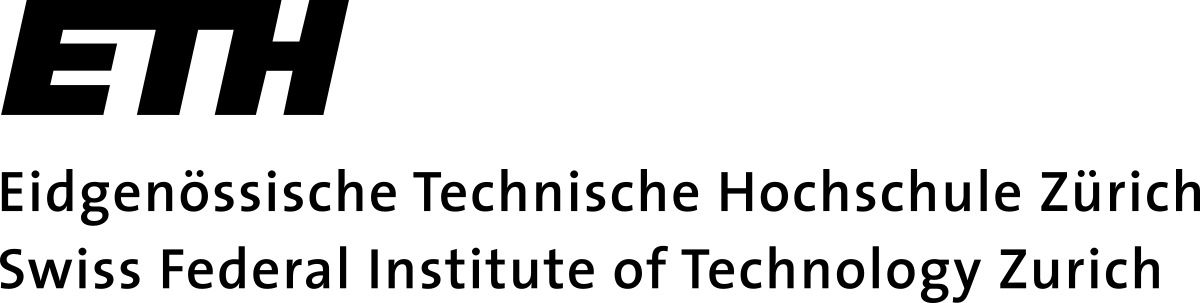
\includegraphics[width=7cm]{resources/logos/ethz logo.png}
\end{subfigure}%
\begin{subfigure}[t]{0.5\mylength}
		\raggedleft
		
\includegraphics[width=7cm]{resources/logos/MIT_logo_2.png}
\end{subfigure}%ghd
\vspace*{-2.3cm}
\end{figure}





\end{center}

\end{titlepage}
\newpage
\thispagestyle{empty}
\mbox{}
\newpage

%%%%%%%%%%%%%%%%%%%%%%%%%%%%%%%%%%%%%%%%%%%%%%%%%%%%%%%%%%%%%%%%%%%%%%%%%
\newpage\thispagestyle{empty}
\selectlanguage{english}
%\afterpage{\blankpage}
\setlength{\parskip}{1em}
\thispagestyle{empty}
\noindent
{\huge \textbf{Acknowledgements}}
\\[1\baselineskip]
\noindent
First acknowledgement.

\noindent
Second acknowledgement.

\noindent
Third acknowledgement.

\setlength{\parskip}{0.3em}
\setlength{\parskip}{0.3em plus 2pt}
\thispagestyle{empty}
\pagenumbering{gobble}
%{\Huge \textbf{Abstract}}
%\newline
\makeatletter
\@openrightfalse
\makeatother
\chapter*{Abstract}

\vspace*{-0.2cm}

A search for the exclusive decays of the Higgs boson to a photon and either a $\phi(1020)$, $\omega(782)$ or $D^{*}(2007)^{0}$ meson is presented. These decays have been suggested as a probe of the Higgs boson couplings to light quarks and as a test of potential deviations from the Standard Model prediction in these flavour interactions. The analysis is performed with a pp collision data sample corresponding to an integrated luminosity of 39.54 fb$^{-1}$ collected at $\sqrt{s}=$13 TeV with the CMS detector at the Large Hadron Collider (LHC) in 2018 during Run 2. Four decay channels are explored: $\text{H}\decaysto \phi\gamma$ with further $\phi\decaysto \pi^+\pi^-\pi^0$, $\text{H}\decaysto \omega\gamma$ with further $\omega\decaysto \pi^+\pi^-\pi^0$, $\text{H}\decaysto D^{*0}\gamma$ with further $D^{*0}\decaysto D^{0}\pi^{0}/\gamma$, $D^{0}\decaysto K^{-}\pi^{+}$ and $\text{H}\decaysto D^{*0}\gamma$ with further $D^{*0}\decaysto D^{0}\pi^{0}/\gamma$, $D^{0}\decaysto K^{-}\pi^{+}\pi^{0}$. Estimated upper limits at a 95\% confidence level on the branching fractions of the four Higgs boson decay modes were obtained, and are $2.2\times10^{-3}$, $2.2\times10^{-3}$, $2.2\times10^{-3}$ and $2.2\times10^{-3}$, respectively.

\vspace*{1.5cm}

Aquesta tesi presenta un estudi sobre desintegracions del bosó de Higgs en un fotó i en un mesó $\phi(1020)$, $\omega(782)$ o $D^{*}(2007)^{0}$. Aquests decaïments han estat proposats com a mètode per mesurar les constants d'acoblament del bosó de Higgs amb els quarks lleugers i també com a prova de possibles desviacions en prediccions del model estàndard de física de partícules. L'anàlisi s'ha realitzat amb una mostra de dades de col·lisions protó-protó corresponent a una lluminositat integrada de 39,54 fb$^{-1}$ recollida a $\sqrt{s}=$13 TeV amb el detector CMS al Gran Col·lisionador d'Hadrons (GCH) l'any 2018 durant la Run 2. S'han estudiat quatre canals de desintegració: $\text{H}\decaysto \phi\gamma$ amb posterior $\phi\decaysto \pi^+\pi^-\pi^0$, $\text{H}\decaysto \omega\gamma$ amb posterior $\omega\decaysto \pi^+\pi^-\pi^0$, $\text{H}\decaysto D^{*0}\gamma$ amb posterior $D^{*0}\decaysto D^{0}\pi^{0}/\gamma$, $D^{0}\decaysto K^{-}\pi^{+}$ i $\text{H}\decaysto D^{*0}\gamma$ amb posterior $D^{*0}\decaysto D^{0}\pi^{0}/\gamma$, $D^{0}\decaysto K^{-}\pi^{+}\pi^{0}$. S'han obtingut estimacions dels límits superiors amb un nivell de confiança del 95\% per a les fraccions de desintegració dels quatre modes estudiats, que són de $2.2\times10^{-3}$, $2.2\times10^{-3}$, $2.2\times10^{-3}$ i $2.2\times10^{-3}$, respectivament.

\vspace*{-0.2cm}


{\let\thefootnote\relax\footnote{Keywords: CERN, LHC, CMS, Higgs boson, rare decays.}}
%https://cran.r-project.org/web/classifications/MSC-2010.html

\setlength{\parskip}{0.0em}
\makeatletter
\@openrighttrue
\makeatother
\pagenumbering{roman} \setcounter{page}{1}
\phantomsection\pdfbookmark{Contents}{contents}%per hyperlink
\tableofcontents
\newpage \thispagestyle{empty}
%%%%%%%%%%%%%%%%%%%%%%%%%%%%%%%%%%%%%%%%%%%%%%%%%%%%%%%%%%%%%%%%%%%%%%%%%
\setlength{\parskip}{0.3em plus 2pt}

%%%%%%%%%%%%%%%%%%%%% això pels headings %%%%%%%%%%%%%%%%%%%%%%%%
\pagestyle{fancy}
\cleardoublepage
\phantomsection
\addcontentsline{toc}{chapter}{Introduction}
\markboth{Introduction}{Introduction}%header right and left
\setcounter{footnote}{0}
\setcounter{figure}{0}
\setcounter{table}{0}
\chapter*{Introduction}

This is the introduction.

\newpage \thispagestyle{empty}

%%%%%%%%%%%%%%%%%%%%%%%%%%%%%%%%%%%%%%%%%%%%%%%%%%%%%%%%%%%%%%%%%%%%%%%%%

\mainmatter
\chapter[Theory and Motivation]{Theory and Motivation}

This chapter aims to provide an overview of the Standard Model of Particle Physics (SM), with a specific focus on the important role played by the Higgs boson. We will give a brief introduction to the SM and its fundamental particles, discuss the Lagrangian that governs their behaviour, and explore their interactions represented by Feynman diagrams. Moreover, we will examine the characteristics of the Higgs boson – its properties, its most frequent production and decay modes, and the Yukawa couplings to the three different fermion families. Finally, we will concentrate on the decay channels subject of our analysis, and explore how a significant discrepancy between the measurements of these decay modes and the SM predictions might lead to new physics beyond the SM.

\section{The Standard Model}

One of the traits that distinguishes humans from other life forms is our sense of curiosity. Since ancient times, we have been trying to explain what happens around us, enabling us to predict and potentially harness the laws of nature. An exceptional theory that has come very close to achieving this goal is the Standard Model of Particle Physics (SM). It stands as one of the most precise theories ever conceived by humanity, and is the most successful theory of particle physics to date. The Standard Model serves as a theory capable of describing three of the four known fundamental forces in the Universe (electromagnetic, weak and strong forces, but not gravity). This is achieved by classifying a set of elementary particles and defining the interactions between them. Summaries of the SM can be found in \cite{Perkins:1982xb, Peskin:1995ev} among many others.

More in detail, the SM is a quantum field theory (QFT) defined by an internal local $\text{SU}(3)_{\text{C}}\times \text{SU}(2)_{\text{L}}\times \text{U}(1)_{\text{Y}}$ gauge symmetry. Each elementary particle has its corresponding field in the theory and is categorized as a fermion or a boson based on its spin (half-integer-spin particles are fermions, whereas integer-spin particles are bosons). There are twelve fermions organized into three families or generations of four members: a charged lepton (e.g., the electron), a neutral lepton (neutrino), an up-type quark and a down-type quark (in addition, each particle has its own corresponding antiparticle) (see Figure \ref{fig:SM}).

\begin{figure}[!ht]
    \vspace*{-0.0cm}
    \centering
    \setlength{\mylength}{\textwidth}
    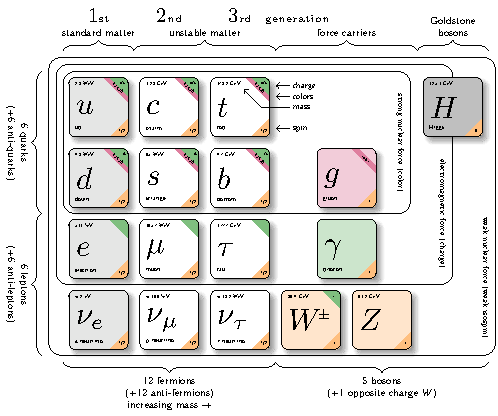
\includegraphics[width=0.84\mylength]{resources/SM_particles/SM_particles.pdf}
    \vspace*{-0.0cm}
    \caption{Elementary particles of the Standard Model. The electric charge, mass and spin of each particle are shown. Figure from \cite{Wongel:2816526}.}
    \label{fig:SM}
    \vspace*{-0.3cm}
\end{figure}
These three factors of the gauge symmetry group give rise to the three fundamental interactions between fermions, which are mediated by gauge bosons. To be precise, each generator of a local invariant gauge group induces a massless gauge boson. In the same way that in quantum electrodynamics (QED), the local gauge invariance of the theory under the $\text{U}(1)$ group leads to the existence of a massless gauge field $A_\mu$ (the photon field), in the SM, the process is analogous.

The invariance of the SM under $\text{SU}(3)_{\text{C}}$ postulates the existence of the gluon. More precisely, the eight generators of $\text{SU}(3)_{\text{C}}$ introduce eight gluons that mediate the strong force between particles that possess color charge (quarks and gluons). This is known as the quantum chromodynamics (QCD) sector of the Standard Model.

Similarly, the invariance of the second and third factors $\text{SU}(2)_{\text{L}}\times \text{U}(1)_{\text{Y}}$ indicates the existence of the photon, the $Z^{0}$ and the $W^{\pm}$ bosons. In this case, unlike in QED or QCD, we cannot directly associate the photon with the generator of the hypercharge group $\text{U}(1)_{\text{Y}}$ and the $Z^{0}$, $W^{\pm}$ bosons with the generators of the left weak isospin group $\text{SU}(2)_{\text{L}}$. Instead, the generators of $\text{SU}(2)_{\text{L}}\times \text{U}(1)_{\text{Y}}$ give rise to four intermediate vector bosons ($W_\mu^{1,2,3}$ for $\text{SU}(2)_{\text{L}}$ and $B_\mu$ for $\text{U}(1)_{\text{Y}}$), which are then mixed through the weak mixing angle or Weinberg angle, $\theta_{\text{W}}$, to produce the physical $\gamma$ ($A_\mu$), $Z^{0}$, $W^{\pm}$. The physical bosons are then defined as:
\begin{align*}
    W_\mu^{\pm} &= \frac{1}{\sqrt{2}}(W_\mu^{1}\mp iW_\mu^{2})\\
    \begin{pmatrix}
        A_\mu \\
        Z^{0}_\mu
    \end{pmatrix}
    &=
    \begin{pmatrix}
        \cos{\theta_{\text{W}}} & \sin{\theta_{\text{W}}} \\
        -\sin{\theta_{\text{W}}} & \cos{\theta_{\text{W}}}
    \end{pmatrix}
    \begin{pmatrix}
        B_\mu \\
        W^{3}_\mu
    \end{pmatrix}
\end{align*}
By the definition of the groups $\text{SU}(2)_{\text{L}}$ and $\text{U}(1)_{\text{Y}}$, the field $W_\mu^{1,2,3}$ couples only to left-handed (negative helicity) particles, whereas the hypercharge field $B_\mu$ couples to both left and right components with the same strength. Therefore, the intermediate boson mixing implies that $W^{\pm}$ only couple to left-handed particles, but $Z^{0}$ couples to both left and right-handed particles with different strengths, inducing (non-maximal) parity violation.

All gauge bosons that arise from the generators of gauge-invariant groups are expected to be massless; otherwise, the principle of local gauge invariance is spoiled and the theory becomes unrenormalizable. However, this contradicts experimental observations, which confirm that the $Z^{0}$ and $W^{\pm}$ bosons are, in fact, massive. This breaking of gauge invariance when giving a mass to a particle is not restricted only to gauge bosons but also happens for fermions. In the SM, to allow for massive fields, all particles obtain their masses using spontaneous symmetry breaking (SSB) via the Higgs mechanism.

Spontaneous symmetry breaking is a fundamental principle of QFT used to explain how gauge bosons (and, in general, massive particles) can acquire non-vanishing mass while maintaining the theory gauge-invariant. This process describes systems where the Lagrangian obeys symmetries, but the lowest-energy vacuum solutions do not exhibit the same symmetries. In the case of the Higgs mechanism, it relies on the existence of an $\text{SU}(2)$ doublet complex scalar field $\phi$ with hypercharge $Y = +1$, which can be written as 
\begin{equation*}
    \phi=
    \begin{pmatrix}
        \phi^{+} \\
        \phi^{0}
    \end{pmatrix}
\end{equation*}
with $(\phi^{+})^{*}=\phi^{-}$ and $(\phi^{0})^{*}=\phi^{0}$. This scalar field has a Lagrangian density given by $\mathcal{L}=\abs{D_{\mu}\phi}^2 - V(\phi)$ and a potential $V(\phi) = \mu^2\phi^\dag\phi+\lambda(\phi^\dag\phi)^2$, where $D_\mu$ is the covariant derivative determined by $\text{SU}(2)_{\text{L}}\times \text{U}(1)_{\text{Y}}$. When expanding the field $\phi$ around a minimum of the potential $V$, one finds out that there are infinitely many values of $\phi$ that minimize the potential. Suppose one expands $\phi$ around
\begin{equation*}
    \phi_{0}=\frac{1}{\sqrt{2}}
    \begin{pmatrix}
        0 \\
        v
    \end{pmatrix},\quad \text{so}\quad
    \phi(x)=\frac{1}{\sqrt{2}}
    \begin{pmatrix}
        0 \\
        v + h(x)
    \end{pmatrix}.
\end{equation*}
Deciding to expand the field around a chosen minimum $\phi_{0}$ spontaneously breaks the $\text{SU}(2)_{\text{L}}\times \text{U}(1)_{\text{Y}}$ symmetry, which in turn generates mass terms for the weak bosons in the Lagrangian. To convince oneself of the last implication it suffices to expand the $\abs{D_{\mu}\phi}^2$ term around the chosen vacuum expectation value $v$, which will produce terms of the form $M_{W}^2W_\mu^{+}W^{-\mu}$ and $M_{Z}^2Z_\mu^{0}Z^{0\mu}$ in the Lagrangian density. This scalar field is called the Higgs field.

With that, the Standard Model of particle physics is governed by the following Lagrangian density:
\begin{equation}
\begin{aligned}
    \mathcal{L}_{\text{SM}} &= -\frac{1}{4}G_{\mu\nu}^{a}G^{a\mu\nu} -\frac{1}{4}W_{\mu\nu}^{i}W^{i\mu\nu} -\frac{1}{4}B_{\mu\nu}B^{\mu\nu} \label{eq:L_SM}\\
    &+ \abs{D_\mu\phi}^2 - \mu^2\phi^\dag\phi - \lambda(\phi^\dag\phi)^2 \\
    &+ i\left[\bar{L}\slashed{D} L + \bar{e}\slashed{D} e + \bar{Q}\slashed{D} Q + \bar{u}\slashed{D} u + \bar{d}\slashed{D} d\right] \\
    & -\left[Y_{e}\bar{L}\phi e + Y_u\bar{Q}\phi^{c} u + Y_d\bar{Q}\phi d + \text{h.c.}\right]
\end{aligned}
\end{equation}
The used notation is the following: $\phi$, $Q$, $u$, $d$, $L$, $e$ are the SM Higgs, quarks and lepton fields. The left-handed doublets are denoted by capital letters as
\begin{equation*}
    Q_{i} = 
    \begin{pmatrix}
    u_{L}^{i}\\
    d_{L}^{i}
    \end{pmatrix}
    \text{ for quarks, and } L_{\alpha} = 
    \begin{pmatrix}
    \nu_{L}^{\alpha}\\
    e_{L}^{\alpha}
    \end{pmatrix}\text{for leptons,}
\end{equation*}
whereas for the right-handed singlets lowercase letters are used. We use the usual covariant derivative defined as
\begin{equation*}
    D_\mu = \partial_\mu - ig_{s}T^{a}G_\mu^{a} - ig\frac{\sigma^{i}}{2}W_\mu^{i} - ig'\frac{Y}{2}B_\mu
\end{equation*}
and where $T^{a}$, $\sigma^{i}$ (Pauli matrices) and $Y$ (weak hypercharge) are the generators of SU(3), SU(2) and SU(1) respectively, and $g_s$, $g$ and $g'$ are the coupling constants. $\phi^{c}$ is the charge conjugate of $\phi$ defined by $\phi^{c} = i\frac{\sigma_{2}}{2}\phi^{\dag}$.

The first line in Equation \eqref{eq:L_SM} describes the kinetic energies and interactions of the gauge boson fields. The field strength tensors associated to $G_\mu^{a}$ (gluons), $W_\mu^{i}$ and $B_\mu$ ($W^{\pm}$, $Z^{0}$, $\gamma$) are defined by
\begin{align*}
    G_{\mu\nu}^{a} &= \partial_\mu G_\nu^{a} - \partial_\nu G_\mu^{a} - g_{s} f^{abc}G_\mu^{b}G_\nu^{c}\\
    W_{\mu\nu}^{i} &= \partial_\mu W_\nu^{i} - \partial_\nu W_\mu^{i} - g \epsilon^{ijk}W_\mu^{j}W_\nu^{k}\\
    B_{\mu\nu} &= \partial_\mu B_\nu - \partial_\nu B_\mu
\end{align*}
where $f^{abc}$ and $\epsilon^{ijk}$ are the group structure constants of SU(3) and SU(2), respectively (the strength tensor of the hypercharge field $B_\mu$ does not have this extra term since U(1) is abelian). This is the origin of gluons and electroweak bosons self-interactions.

The second line in Equation \eqref{eq:L_SM} describes the Higgs field and generates the masses of the weak gauge bosons $W^{\pm}$, $Z^{0}$ and of the Higgs boson. In particular, the term $\abs{D_{\mu}\phi}^2$ generates all interactions between the gauge bosons and the Higgs field.

The third line in Equation \eqref{eq:L_SM} is responsible for fermion kinetic energies as well as their interactions with all bosons (gluons and eletroweak bosons). We have five terms: left-handed lepton doublets, right-handed lepton singlets (only charged leptons since right-handed neutrinos do not couple in the SM), left-handed quark doublets, right-handed up-type quark singlets and right-handed down-type quark singlets. The covariant derivative terms relative to each group apply only to these fermions that transform under that group. For instance, the first term would expand as
\begin{equation*}
    i\bar{L}\slashed{D} L = i\bar{L}\gamma^{\mu}D_\mu L = i
    \begin{pmatrix}
        \bar{\nu}_{L}^{\alpha} & \bar{e}_{L}^{\alpha}
    \end{pmatrix}
    \gamma^{\mu}\left(\partial_\mu - ig\frac{\sigma^{i}}{2}W_\mu^{i} - ig'\frac{Y}{2}B_\mu\right)
    \begin{pmatrix}
        \nu_{L}^{\alpha}\\
        e_{L}^{\alpha}
    \end{pmatrix},
\end{equation*}
since the leptons do not carry color charge, but the fourth term would expand as
\begin{equation*}
    i\bar{u}\slashed{D} u = i\bar{u}\gamma^{\mu}D_\mu u = i \bar{u}_{R}^{i}
    \gamma^{\mu}\left(\partial_\mu - ig_{s}T^{a}G_\mu^{a} - ig'\frac{Y}{2}B_\mu\right) u_{R}^{i},
\end{equation*}
because the right-handed quark is a singlet under SU(2)$_{\text{L}}$.

Finally, the couplings between the Higgs boson and the fermions, and in turn fermion masses, are generated by the fourth line in Equation \eqref{eq:L_SM}. These terms are gauge invariant, but give rise to fermion masses. For example, for the leptons and taking the Higgs field expansion around $\phi_0$, the first term will expand as
\begin{equation*}
    Y_{e}\bar{L}\phi e = \frac{Y_e^{\alpha\beta}}{\sqrt{2}}
    \begin{pmatrix}
        \bar{\nu}_{L}^{\alpha} & \bar{e}_{L}^{\alpha}
    \end{pmatrix}
    \begin{pmatrix}
        0\\
        v + h(x)
    \end{pmatrix}
    e_{R}^{\beta} = \frac{Y_e^{\alpha\beta}}{\sqrt{2}}\left[v + h(x)\right] \bar{e}_{L}^{\alpha}e_{R}^{\beta}
\end{equation*}
which in addition to its hermitian conjugate will ultimately yield the term
\begin{equation*}
    \frac{Y_e^{\alpha\beta}}{\sqrt{2}} v \left[\bar{e}_{L}^{\alpha}e_{R}^{\beta} + \bar{e}_{R}^{\alpha}e_{L}^{\beta}\right] = \frac{Y_e^{\alpha\beta}v}{\sqrt{2}} \bar{e}^{\alpha}e^{\beta}
\end{equation*}
after spontaneous symmetry breaking. One can easily identify the mass of the three charged leptons as
\begin{equation*}
    m_{e} = \frac{Y_e^{ee} v}{\sqrt{2}},\quad m_{\mu} = \frac{Y_e^{\mu\mu} v}{\sqrt{2}}\quad\text{and}\quad m_{\tau} = \frac{Y_e^{\tau\tau} v}{\sqrt{2}}.
\end{equation*}
To generate mass terms for up-type like quarks the Yukawa term involves the charge conjugate of the Higgs doublet (as in the second term of the fourth line in Equation \eqref{eq:L_SM}).

The Standard Model Lagrangian in Equation \eqref{eq:L_SM} governs the interactions between all particles within the theory. These interactions can be represented as vertices in Feynman diagrams. The vertices shown in Figure \ref{fig:SM_vertices} are all possible interactions in the SM, and are constructed from the terms in the SM Lagrangian. Terms that, after SSB, involve only two fields do not result in vertices as they are interpreted as mass terms. Consequently, we only see vertices with at least three fields.

For instance, to derive the QED vertex for the electron, one must expand the terms $i\left(\bar{L}\slashed{D} L + \bar{e}\slashed{D} e\right)$ and keep the terms of the form $\bar{e}\cdot\ldots\cdot e$. This expansion ultimately yields two contributions. The first one corresponds to the coupling of the electron to the photon field:
\begin{equation}
    \label{eq:qed_term}
    -\frac{gg'}{\sqrt{{g'}^2 + g^2}}\bar{e}\gamma^\mu eA_\mu = -e \bar{e}\gamma^\mu eA_\mu\ .
\end{equation}
The first $e$ in the latter expression refers to the electrical charge, therefore connecting both couplings $g$ and $g'$ with the electrical charge and the weak mixing angle, yielding $e=g'\cos{\theta_{\text{W}}}=g\sin{\theta_{\text{W}}}$. The second term that arises corresponds to the $Z^0$ boson:
\begin{equation*}
    \frac{1}{\sqrt{{g'}^2 + g^2}}\left(\frac{{g'}^2 - g^2}{2}\bar{e}_{L}\gamma^\mu e_{L} + {g'}^2 \bar{e}_{R}\gamma^\mu e_{R}\right)Z^0_\mu \ .
\end{equation*}
We can see that the $Z^0$ couples to both left-handed and right-handed components of the electron but with different strengths. Hence, by removing the fields from Equation \eqref{eq:qed_term} and multiplying by $i$, the coupling of the electron to the photon associated with the QED vertex is
\begin{equation}
    \label{eq:qed_vertex}
\vcenter{\hbox{
\setlength{\mylength}{\textwidth}
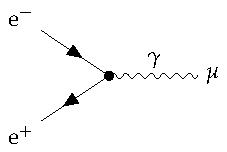
\includegraphics[height=0.16\mylength]{resources/SM_vertices/qed.pdf}
 }} = -ie \gamma^\mu \ .
\end{equation}
Each of the vertices in Figure \ref{fig:SM_vertices} has an associated factor that can be computed from the SM Lagrangian density in a similar manner. Therefore, we can observe, for example, that the Higgs boson does not couple to the photon or the gluon field, and that there is no direct interaction between three fermions.

\begin{figure}[!ht]
    \captionsetup[subfigure]{labelformat=empty}
    \vspace*{-0.2cm}
    \centering
    \setlength{\mylength}{\textwidth}
    \begin{subfigure}[t]{0.33\mylength}
            \centering
            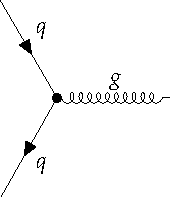
\includegraphics[height=0.20\mylength]{resources/SM_vertices/v1.pdf}
            \setlength{\unitlength}{0.25\mylength}
            %\caption{\footnotesize (a)}
    \end{subfigure}%
    \begin{subfigure}[t]{0.33\mylength}
            \centering
            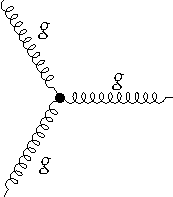
\includegraphics[height=0.20\mylength]{resources/SM_vertices/v2.pdf}
            \setlength{\unitlength}{0.25\mylength}
            %\caption{\footnotesize (b)}
    \end{subfigure}%
    \begin{subfigure}[t]{0.33\mylength}
            \centering
            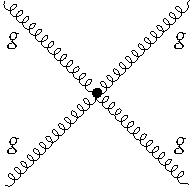
\includegraphics[height=0.20\mylength]{resources/SM_vertices/v3.pdf}
            \setlength{\unitlength}{0.25\mylength}
            %\caption{\footnotesize (c)}
    \end{subfigure}%\begin{subfigure}[t]{0.33\mylength}\baselineskip    
    \vskip\baselineskip
    \vspace*{-0.1cm}
    \begin{subfigure}[t]{0.33\mylength}
            \centering
            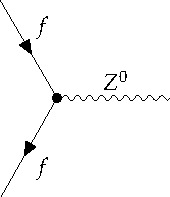
\includegraphics[height=0.20\mylength]{resources/SM_vertices/v4.pdf}
            \setlength{\unitlength}{0.25\mylength}
            %\caption{\footnotesize (d)}
    \end{subfigure}%\begin{subfigure}[t]{0.33\mylength}
    \begin{subfigure}[t]{0.33\mylength}
            \centering
            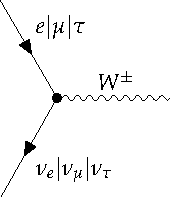
\includegraphics[height=0.20\mylength]{resources/SM_vertices/v5.pdf}
            \setlength{\unitlength}{0.25\mylength}
            %\caption{\footnotesize (e)}
    \end{subfigure}%\begin{subfigure}[t]{0.33\mylength}
    \begin{subfigure}[t]{0.33\mylength}
            \centering
            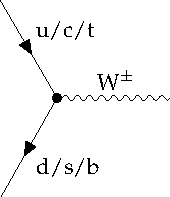
\includegraphics[height=0.20\mylength]{resources/SM_vertices/v6.pdf}
            \setlength{\unitlength}{0.25\mylength}
            %\caption{\footnotesize (f)}
    \end{subfigure}%
    \vskip\baselineskip
    \vspace*{-0.1cm}
    \begin{subfigure}[t]{0.33\mylength}
            \centering
            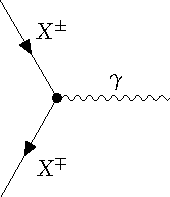
\includegraphics[height=0.20\mylength]{resources/SM_vertices/v7.pdf}
            \setlength{\unitlength}{0.25\mylength}
            %\caption{\footnotesize (g)}
    \end{subfigure}%\begin{subfigure}[t]{0.33\mylength}
    \begin{subfigure}[t]{0.33\mylength}
            \centering
            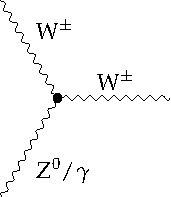
\includegraphics[height=0.20\mylength]{resources/SM_vertices/v8.pdf}
            \setlength{\unitlength}{0.25\mylength}
            %\caption{\footnotesize (h)}
    \end{subfigure}%\begin{subfigure}[t]{0.33\mylength}
    \begin{subfigure}[t]{0.33\mylength}
            \centering
            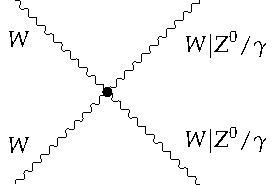
\includegraphics[height=0.20\mylength]{resources/SM_vertices/v9.pdf}
            \setlength{\unitlength}{0.25\mylength}
            %\caption{\footnotesize (i)}
    \end{subfigure}%
    \vskip\baselineskip
    \vspace*{-0.1cm}
    \begin{subfigure}[t]{0.33\mylength}
            \centering
            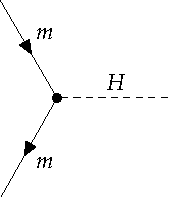
\includegraphics[height=0.20\mylength]{resources/SM_vertices/v10.pdf}
            \setlength{\unitlength}{0.25\mylength}
            %\caption{\footnotesize (j)}
    \end{subfigure}%\begin{subfigure}[t]{0.33\mylength}
    \begin{subfigure}[t]{0.33\mylength}
            \centering
            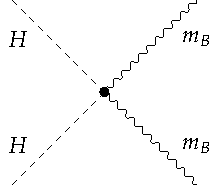
\includegraphics[height=0.20\mylength]{resources/SM_vertices/v11.pdf}
            \setlength{\unitlength}{0.25\mylength}
            %\caption{\footnotesize (k)}
    \end{subfigure}%\begin{subfigure}[t]{0.33\mylength}
    \vspace*{-0.0cm}
    \caption{All possible interactions in the Standard Model, represented by Feynman diagrams. $q$ is any quark, $g$ is (any) gluon, $X^{\pm}$ is any charged particle, $\gamma$ is a photon, $f$ is any fermion, $m$ is any massive particle (except neutrinos), $m_{B}$ is any massive boson. In diagrams with multiple particle labels separated by / one particle label is chosen. In diagrams with particle labels separated by | the labels must be chosen in the same order. For example, in the four electroweak boson case the valid diagrams are $WWWW$, $WWZZ$, $WW\gamma\gamma$ and $WWZ\gamma$.}
    \label{fig:SM_vertices}
    \vspace*{-0.2cm}
\end{figure}

The Standard Model has proven to predict numerous measurements with exceptional precision. Yet, the theory does not explain why the masses of all particles are given by the values we measure. In fact, aside from the mass of the photon, which is protected by the unbroken U(1) gauge symmetry of QED, the SM does not predict any other mass value. All fermion masses (or equivalently, the Yukawa couplings) are free parameters of the theory.

While this theory has been remarkably successful, it cannot serve as the final theory of nature, as numerous unresolved puzzles persist. Many cosmological observations remain unaccounted for by the SM, such as the baryon-antibaryon asymmetry, the behaviour of gravity as described by General Relativity, the accelerated expansion of the Universe — potentially described by dark energy — and the absence of a suitable candidate for dark matter. Furthermore, the SM fails to explain the non-vanishing mass of the neutrinos as a consequence of neutrino flavour oscillation. In pursuit of a superior theory capable of encompassing the SM as well as these (and many other) discrepancies, the physics community is thoroughly trying to ``break'' the Standard Model to unveil hints towards an ultimate theory.

\section{The Higgs boson}

In 1964, Peter Higgs, along with five other theoretical physicists, proposed the Higgs mechanism to explain how certain particles (fermions and weak bosons) might acquire mass in local gauge theories \cite{Higgs:1964pj,Englert:1964et,Guralnik:1964eu}. If these ideas were correct, a spin-0 particle (namely the Higgs boson) should exist and possess some well-defined properties. Nearly 50 years later, on the 4\textsuperscript{th} of July 2012, a scalar particle consistent with the Higgs boson was discovered at the LHC by the CMS and ATLAS collaborations \cite{CMS:2012qbp,ATLAS:2012yve}.

\subsection{Properties of the Higgs boson}

The Higgs boson is a weak isospin SU(2)$_{\text{L}}$ doublet, massive scalar neutral boson. Table \ref{tab:higgs_properties} summarizes the SM predicted properties \cite{Djouadi:2005gi, LHCHiggsCrossSectionWorkingGroup:2016ypw} as well as the measured properties of the Higgs boson from the Particle Data Group (PDG) \cite{PDG}.

\begin{table}[ht]
    \centering
    \begin{tabular}{|l|l|l|}
        \hline
        \cellcolor{lightgray}Property & \cellcolor{lightgray}SM prediction & \cellcolor{lightgray}Mesasured value \\ \hline
        Mass                & $m \lesssim 700 \;\; \text{GeV}$ & $m = 125.25 \pm 0.17 \;\; \text{GeV}$             \\
        Spin                &  $J=0$ & $J=0$                                             \\
        Electric charge     & $q=0$  & $q=0$                                             \\
        Full width          & $\Gamma = 4.12 \pm 0.06 \;\;  \text{MeV}$  & $\Gamma = 3.2^{+2.8}_{-2.2} \;\;  \text{MeV}$     \\
        Lifetime            & $\tau = (1.60 \pm 0.02) \times 10^{-22} \;\;  \text{s}$  & $\tau = 2.1^{+4.5}_{-1.0} \times 10^{-22} \;\;  \text{s}$   \\ \hline
    \end{tabular}
    \caption{Properties of the Higgs boson. The SM prediction for the full width and the lifetime depend on the Higgs mass, which is assumed to be $m = 125.25$ GeV.}
    \label{tab:higgs_properties}
\end{table}

As stated previously, the SM does not predict the mass of any particle (except for the photon), including the mass of the Higgs boson. Nevertheless, some theoretical arguments, such as radiative corrections and unitarity considerations, enabled theorists to establish upper bounds on the Higgs mass \cite{Djouadi:2005gi}.

\subsection{Main production modes of the Higgs boson}

To understand the production and decay modes of the Higgs boson, it's important to recall that the Higgs boson couples to all the other massive particles of the SM (it couples to the gauge bosons via the $\abs{D_{\mu}\phi}^2$ term in the Higgs part of the SM Lagrangian and to fermions via the Yukawa couplings), as well as to itself. Expanding the terms in the Lagrangian reveals that the coupling between the Higgs boson and any fermion is directly proportional to the particle's rest mass, while the coupling between the Higgs boson and any massive vector boson is directly proportional to the square of the particle's rest mass.

Collecting the relevant Feynman vertices, one can determine the dominant production modes for the Higgs boson, as shown in Figure \ref{fig:Higgs_production}. Since the heavier the particle, the stronger its Higgs coupling constant is, we observe that in most cases, the particles involved in the vertex where the Higgs boson is produced are very heavy (top and bottom quarks and massive gauge bosons).

\begin{figure}[!ht]
    \captionsetup[subfigure]{labelformat=empty}
    \vspace*{-0.2cm}
    \centering
    \setlength{\mylength}{\textwidth}
    \begin{subfigure}[t]{0.33\mylength}
            \centering
            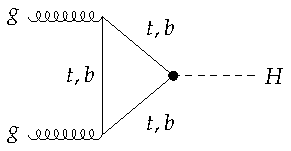
\includegraphics[height=0.16\mylength]{resources/H_production_diagrams/v1.pdf}
            \setlength{\unitlength}{0.25\mylength}
            \caption{\footnotesize (a)}
    \end{subfigure}%
    \begin{subfigure}[t]{0.33\mylength}
            \centering
            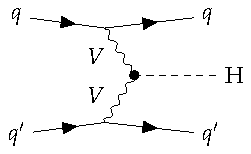
\includegraphics[height=0.16\mylength]{resources/H_production_diagrams/v2.pdf}
            \setlength{\unitlength}{0.25\mylength}
            \caption{\footnotesize (b)}
    \end{subfigure}%
    \begin{subfigure}[t]{0.33\mylength}
            \centering
            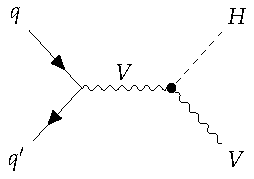
\includegraphics[height=0.185\mylength]{resources/H_production_diagrams/v3.pdf}
            \setlength{\unitlength}{0.25\mylength}
            \caption{\footnotesize (c)}
    \end{subfigure}%\begin{subfigure}[t]{0.33\mylength}\baselineskip    
    \vskip\baselineskip
    \vspace*{-0.1cm}
    \begin{subfigure}[t]{0.33\mylength}
            \centering
            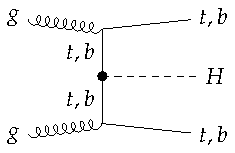
\includegraphics[height=0.16\mylength]{resources/H_production_diagrams/v4.pdf}
            \setlength{\unitlength}{0.25\mylength}
            \caption{\footnotesize (d)}
    \end{subfigure}%\begin{subfigure}[t]{0.33\mylength}
    \begin{subfigure}[t]{0.33\mylength}
            \centering
            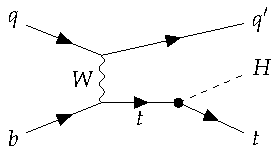
\includegraphics[height=0.16\mylength]{resources/H_production_diagrams/v5.pdf}
            \setlength{\unitlength}{0.25\mylength}
            \caption{\footnotesize (e)}
    \end{subfigure}%\begin{subfigure}[t]{0.33\mylength}
    \begin{subfigure}[t]{0.33\mylength}
            \centering
            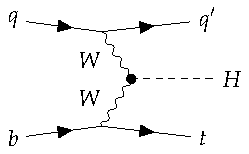
\includegraphics[height=0.16\mylength]{resources/H_production_diagrams/v6.pdf}
            \setlength{\unitlength}{0.25\mylength}
            \caption{\footnotesize (f)}
    \end{subfigure}%
    \vspace*{-0.0cm}
    \caption{Higgs boson production in (a) gluon-gluon fusion (ggH), (b) vector boson fusion (VBF), (c) associated production with a $W$ or $Z$ (V) boson (VH), also known as Higgsstrahlung, (d) associated production with a top or bottom quark pair (ttH or bbH), or tt fusion, and (e, f) associated production with a single top quark (tH).}
    \label{fig:Higgs_production}
    \vspace*{-0.0cm}
\end{figure}

Despite being a second-order process (it requires a heavy quark loop), the strong coupling to heavy quarks makes gluon fusion the process that contributes the most to the production of the Higgs boson at the LHC, a proton-proton collider. The LHC is a gluon-gluon collider when it comes to Higgs production, as gluons dominate the production of Higgs bosons with a mass of around 125 GeV. The second most important process at the LHC is vector boson fusion, where two fermions collide and exchange a virtual vector boson, which radiates a Higgs boson. The third contribution to Higgs boson production, and the first one at LEP, is associated production with a vector boson or Higgsstrahlung. In this production mode, a fermion and antifermion collide and can form a virtual $W^{\pm}$ or $Z^0$ boson which, if it carries enough energy, can emit a Higgs boson.

\todo{Add Higgs production signatures}

To compare the different production cross sections with the SM predictions, we introduce some important quantities to describe interactions at particle colliders. The \textit{center-of-mass energy} $\sqrt{s}$ describes the combined energy of the collided particle beams and is defined as the square root of the Mandelstam variable
\begin{equation*}
\sqrt{s} = \sqrt{(p_1+p_2)^2}\ ,
\end{equation*}
where $p_1$ and $p_2$ are the four-momenta of the two particles. When colliding elementary particles (e.g., $e^+e^-$), the center-of-mass energy is precisely the available energy to produce particles in the collision. When colliding composite particles (e.g., protons), however, the available energy to produce particles is slightly less due to the parton distribution functions within the proton, and there is an energy spread. The \textit{cross section} $\sigma$ of a process describes the likelihood of a specific final state, as a measure of the effective area or target size for a particular interaction. It is measured in units of area, usually barns, defined as barn $= 10^{-28}$ cm$^{2}$. The number of events per unit time can be expressed in terms of the \textit{instantaneous luminosity} $\mathscr{L}$ and the cross section of the studied event $\sigma$ as
\begin{equation*}
    \frac{\d N_{\text{events}}}{\d t} = \mathscr{L}\sigma\ ,
\end{equation*}
and the \textit{integrated luminosity} is defined as 
\begin{equation*}
    L = \int\mathscr{L}\d t\ .
\end{equation*}
Finally, the \textit{signal strength} $\mu$ expresses a measured cross section divided by the expected SM value.

Having established these fundamental concepts, we can now compare the theoretical and measured cross sections for the production of the Higgs boson. Our analysis uses 2018 data from the LHC, with a center-of-mass energy of $\sqrt{s} = 13$ TeV and an integrated luminosity of $L=39.50$ fb$^{-1}$. According to the SM, the total Higgs boson cross section at a center-of-mass energy of $\sqrt{s} = 13$ TeV is $\sigma = 55500 \pm 2800$ fb \cite{LHCHiggsCrossSectionWorkingGroup:2016ypw}, with around 87\% coming from gluon fusion, 7\% from vector boson fusion and 4\% from Higgsstrahlung. The predicted and measured cross section of the Higgs boson at $\sqrt{s} = 13$ TeV from different production modes are shown in Table \ref{tab:Higgs_production}.

\begin{table}[ht]
    \centering
    \begin{tabular}{|l|c|c|c|}
        \hline
        \multicolumn{1}{|c|}{\cellcolor{lightgray}Production mode} & \cellcolor{lightgray} SM $\sigma$ [fb] & \cellcolor{lightgray} Measured $\sigma$ [fb] & \cellcolor{lightgray} Measured $\mu$ \\ \hline
        ggH                         & $48400 \pm 2440$          & $47000 \pm 4500$          & $0.97 \pm 0.08$           \\
        VBF                         & $3774 \pm 81$             & $3020 \pm 460$            & $0.80 \pm 0.12$    \\
        WH                          & $1365  \pm 28$            & $2030  \pm 360$           & $1.49 \pm 0.26$     \\
        %W$^+$H ($W^+\to l^+\nu$)    & $3\times(93.7  \pm 1.8)$  & $0.0  \pm 0.0$        \\
        %W$^+$H                      & $835  \pm 17$             & $0.0  \pm 0.0$        \\
        %W$^-$H ($W^-\to l^-\nu$)    & $3\times(59.4  \pm 1.2)$  & $0.0  \pm 0.0$        \\
        %W$^-$H                      & $530  \pm 11$             & $0.0  \pm 0.0$        \\
        Z$^0$H                      & $879  \pm 36$             & $1130  \pm 220$           & $1.29 \pm 0.24$    \\
        %Z$^0$H ($Z^0\to l^-l^+$)    & $3\times(29.7  \pm 1.2)$  & $0.0  \pm 0.0$        \\
        %ggZ$^0$H ($Z^0\to l^-l^+$)  & $3\times(93.7  \pm 1.8)$  & $0.0  \pm 0.0$        \\
        %Z$^0$H ($Z^0\to \nu\bar{\nu}$)& $3\times(177  \pm 7)$  & $0.0  \pm 0.0$        \\
        %ggZ$^0$H ($Z^0\to \nu\nu$)  & $3\times(93.7  \pm 1.8)$  & $0.0  \pm 0.0$        \\
        ttH + H                     & $582  \pm 61$             & $660  \pm 130$             & $1.13 \pm 0.18$    \\
        %ttH                        & $505  \pm 50$            & $0.0  \pm 0.0$        \\
        bbH                         & $484  \pm 116$            & -       & - \\ \hline
        %tH + tbarH (s and t channels)                  & $77  \pm 12$            & $0.0  \pm 0.0$        \\ \hline
    \end{tabular}
    \caption{Cross section of the Higgs boson's most frequent production modes at $\sqrt{s} = 13$ TeV. SM values from \cite{LHCHiggsCrossSectionWorkingGroup:2016ypw}, measured $\mu$ values from \cite{CMS:2022dwd}, and measured $\sigma$ from $\sigma=\mu\sigma_{\text{SM}}$. At the moment of this writing, the bbH production channel has not been measured yet.}
    \label{tab:Higgs_production}
\end{table}

Since the most significant Higgs boson production channel is gluon fusion, within the limited timeframe of this project, our primary focus will be on this production mode. However, other modes, such as vector boson fusion or associated production with a $W$/$Z$ boson, share reasonable similarities with ggH in terms of implementation and could be further extensions of this analysis.

\subsection{Main decay channels of the Higgs boson}

The Higgs boson is a very short-lived particle, decaying almost instantaneously after its production into lighter particles. According to the couplings of the Higgs field to all other SM particles, at the first loop order, the Higgs boson predominantly decays to the most massive particles that are kinematically accessible. However, there are certain decay modes where the Higgs boson decays into massless particles, such as gluon or photon pairs, as the first-loop contributions are not negligible. Figure \ref{fig:Higgs_decays} shows the most relevant Feynman diagrams for the Higgs boson decay, while Table \ref{tab:Higgs_decays} presents the most frequent decay channels for the Higgs boson, comparing the SM predicted value to the measured value for every decay mode.

\begin{figure}[!ht]
    \captionsetup[subfigure]{labelformat=empty}
    \vspace*{-0.2cm}
    \centering
    \setlength{\mylength}{\textwidth}
    \begin{subfigure}[t]{0.5\mylength}
            \centering
            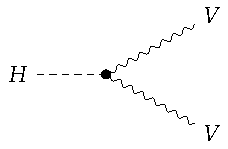
\includegraphics[height=0.1539\mylength]{resources/H_decay_diagrams/v1.pdf}
            \setlength{\unitlength}{0.25\mylength}
            \caption{\footnotesize (a)}
    \end{subfigure}%
    \begin{subfigure}[t]{0.5\mylength}
            \centering
            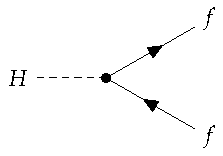
\includegraphics[height=0.1539\mylength]{resources/H_decay_diagrams/v2.pdf}
            \setlength{\unitlength}{0.25\mylength}
            \caption{\footnotesize (b)}
    \end{subfigure}%
    \vskip\baselineskip
    \vspace*{-0.1cm}
    \begin{subfigure}[t]{0.33\mylength}
            \centering
            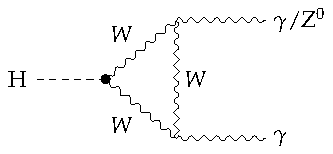
\includegraphics[height=0.1539\mylength]{resources/H_decay_diagrams/v3.pdf}
            \setlength{\unitlength}{0.25\mylength}
            \caption{\footnotesize (c)}
    \end{subfigure}%\begin{subfigure}[t]{0.5\mylength}
    \begin{subfigure}[t]{0.33\mylength}
            \centering
            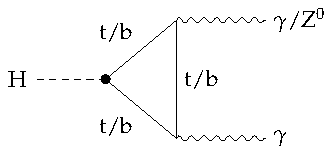
\includegraphics[height=0.1539\mylength]{resources/H_decay_diagrams/v4.pdf}
            \setlength{\unitlength}{0.25\mylength}
            \caption{\footnotesize (d)}
    \end{subfigure}%\begin{subfigure}[t]{0.5\mylength}
    \begin{subfigure}[t]{0.33\mylength}
            \centering
            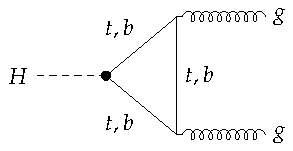
\includegraphics[height=0.1539\mylength]{resources/H_decay_diagrams/v5.pdf}
            \setlength{\unitlength}{0.25\mylength}
            \caption{\footnotesize (e)}
    \end{subfigure}%\begin{subfigure}[t]{0.5\mylength}
    \vspace*{-0.0cm}
    \caption{Higgs boson decays into (a) heavy vector boson pairs ($V$ is $Z^{0}/W^{\pm}$), (b) fermion-antifermion pairs, (c, d) photon pairs or $Z^0\gamma$, and (e) gluon pairs.}
    \label{fig:Higgs_decays}
    \vspace*{-0.0cm}
\end{figure}

\begin{table}[!ht]
    \centering
    \begin{tabular}{|l|c|c|cc|}
        \hline
        \multicolumn{1}{|c|}{\cellcolor{lightgray}Decay channel} & \cellcolor{lightgray} SM $\mathcal{B}$ (\%) & \cellcolor{lightgray} Measured $\mathcal{B}$ (\%) & \multicolumn{2}{c|}{\cellcolor{lightgray} Measured $\mu$} \\ \hline
        $\text{H}\decaysto b\bar{b}$     & $57.8 \pm 0.7$        & $60 \pm 12$         & $1.04 \pm 0.20$ & \cite{CMS:2018nsn}  \\
        $\text{H}\decaysto WW^*$         & $21.8 \pm 0.3$        & $20.7 \pm 2.1$      & $0.95 \pm 0.09$ & \cite{CMS:2022uhn}  \\
        $\text{H}\decaysto gg$           & $8.2 \pm 0.4$         & -    & -  &\\
        $\text{H}\decaysto \tau^+\tau^-$ & $6.23 \pm 0.10$       & $6.1 \pm 1.1$       & $0.98 \pm 0.18$ & \cite{CMS:2017zyp}  \\
        $\text{H}\decaysto c\bar{c}$     & $2.87 \pm 0.16$       & $<40$               & $<14$ & \cite{CMS:2022psv}            \\
        $\text{H}\decaysto ZZ^*$         & $2.68 \pm 0.04$       & $2.6 \pm 0.3$       & $0.97 \pm 0.12$ & \cite{CMS:2022dwd}  \\
        $\text{H}\decaysto \gamma\gamma$ & $0.227 \pm 0.005$     & $0.254 \pm 0.021$   & $1.12 \pm 0.09$ & \cite{CMS:2021kom}  \\
        $\text{H}\decaysto Z\gamma$      & $0.155 \pm 0.009$     & $0.37 \pm 0.14$     & $2.4 \pm 0.9$ & \cite{CMS:2022ahq}    \\
        $\text{H}\decaysto s\bar{s}$     & $0.025 \pm 0.001$     & -                   & - &            \\
        $\text{H}\decaysto \mu^+\mu^-$   & $0.0216 \pm 0.0004$   & $0.026 \pm 0.009$   & $1.19 \pm 0.43$ & \cite{CMS:2020xwi}  \\ \hline
    \end{tabular}
    \caption{Most frequent decay modes of the Higgs boson. SM values from \cite{LHCHiggsCrossSectionWorkingGroup:2016ypw, CMS:2022dwd}, and measured $\mathcal{B}$ from $\mathcal{B}=\mu\mathcal{B}_{\text{SM}}$. At the moment of this writing, the $\text{H}\protect\decaysto gg$ and $\text{H}\protect\decaysto s\bar{s}$ decay channels have not been measured yet.}
    \label{tab:Higgs_decays}
\end{table}

The predicted values by the SM in Table \ref{tab:Higgs_decays} are of significant interest, and there are some remarks worth mentioning.

Firstly, it is observed that there is no decay $\text{H}\decaysto t\bar{t}$. This is because the Higgs boson is lighter than the top quark, $M_H = 125$ GeV < $m_t = 173$ Gev, making it not massive enough to produce a top-antitop quark pair. In fact, the Higgs boson can not even create one real top quark and one virtual top quark. Consequently, the presence of top quarks in the Higgs boson decays is limited to virtual loops, as the ones present in diagrams (d) and (e) of Figure \ref{fig:Higgs_decays}.

Let us examine the branching ratios in Table \ref{tab:Higgs_decays} more closely, starting with the fermionic decays. The Higgs-fermion vertex has a factor of
\begin{equation}
    \label{eq:higgs_fermion_vertex}
\vcenter{\hbox{
\setlength{\mylength}{\textwidth}
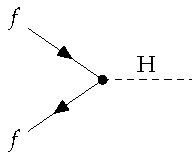
\includegraphics[height=0.16\mylength]{resources/SM_vertices/higgs_fermion.pdf}
 }} = -i \frac{m_f}{v} \ ,
\end{equation}
thus at first approximation, the expected decay width at tree level can be estimated as proportional to
\begin{equation}
\label{eq:Higgs_approx_fermions}
\Gamma(H\decaysto f\bar{f}) \propto N_C m_f^2 \ ,
\end{equation}
where $N_C$ is the number of colours (3 for quarks, 1 for leptons). It is important to note that the mass to use in the above expression is the \textit{running mass} of the particle at an energy scale of $\mu=M_{H}$, rather than the ones presented in Figure \ref{fig:SM}\footnote{The masses of the quarks that are typically provided, for example, in \cite{PDG}, are $m_u(\mu = 2\ \GeV)$, $m_d(\mu = 2\ \GeV)$, $m_s(\mu = 2\ \GeV)$, $m_c(\mu = m_c)$, $m_b(\mu = m_b)$. The $t$-quark mass is determined from event kinematics, see \cite{PDG}. The differences in the masses at the Higgs energy scale compared to the ``usual'' values are more pronounced for heavy quarks. For more information on running masses refer to \cite{Huang:2020hdv}.}. Using the running masses of the particles (for precise values of the running masses, see \cite{Huang:2020hdv}) and the approximation presented above, we obtain the following relation of decay widths for the quarks, taking $\Gamma(H\decaysto s\bar{s}) = 1$:
\begin{equation*}
    \Gamma(H\decaysto b\bar{b}):\Gamma(H\decaysto c\bar{c}):\Gamma(H\decaysto s\bar{s}) \approx  2834:136:1\ ,
\end{equation*}
while the full SM computation yields
\begin{equation*}
    \Gamma(H\decaysto b\bar{b}):\Gamma(H\decaysto c\bar{c}):\Gamma(H\decaysto s\bar{s}) =  2312:115:1\ .
\end{equation*}
The approximation in Equation \eqref{eq:Higgs_approx_fermions} is even better for leptons:
\begin{equation*}
    \Gamma(H\decaysto \tau^+\tau^-):\Gamma(H\decaysto \mu^+\mu^-) \approx  288.53:1\ ,
\end{equation*}
while the full SM computation is remarkably close, giving
\begin{equation*}
    \Gamma(H\decaysto \tau^+\tau^-):\Gamma(H\decaysto \mu^+\mu^-) =  288.43:1\ .
\end{equation*}
The discrepancies between this initial approximation and the results from the SM in Table \ref{tab:Higgs_decays} arise from phase space factors, higher-order Feynman diagrams, and, in the case of quarks, QCD corrections.

For vector bosons, the vertex has a factor of
\begin{equation}
    \label{eq:higgs_boson_vertex}
\vcenter{\hbox{
\setlength{\mylength}{\textwidth}
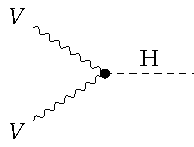
\includegraphics[height=0.16\mylength]{resources/SM_vertices/higgs_boson.pdf}
 }} = 2i \frac{M_V^2}{v}g^{\mu\nu} \ ,
\end{equation}
and similarly, one can estimate the expected decay width at tree level as proportional to
\begin{equation}
    \label{eq:Higgs_approx_bosons}
\Gamma(H\decaysto VV) \propto M_V^4 \ .
\end{equation}
When we compute the same relations as for the fermions we obtain
\begin{equation*}
    \Gamma(H\decaysto WW^*):\Gamma(H\decaysto ZZ^*) \approx  0.604:1\ ,
\end{equation*}
while the full SM computation differs by almost a factor of 14:
\begin{equation*}
    \Gamma(H\decaysto WW^*):\Gamma(H\decaysto ZZ^*) =  8.134:1\ .
\end{equation*}
Despite the vertex in Equation \eqref{eq:higgs_boson_vertex} suggesting that $\Gamma(H\decaysto WW^*) < \Gamma(H\decaysto ZZ^*)$ due to $M_W < M_Z$, other factors play a more significant role in the decay width than just the vertex factors in the boson decays. First of all, the phase space of the decay into $Z^0$ bosons includes an extra $\frac{1}{2}$ symmetry factor due to the decay involving two identical particles. The remaining factor of 7 arises from the inclusion of higher-order Feynman diagrams and, most significantly, from the phase space contribution. The latter contribution quantifies the number of valid momentum and energy configurations for the outgoing particles while still obeying the conservation of energy and momentum.

Note that $2M_W, 2M_Z > M_H > M_W, M_Z$, so for the Higgs boson to decay into two electroweak bosons, one of them must be \textit{off-shell} or \textit{virtual} (that is why one of them is marked with an asterisk). Off-shell or virtual particles do not need to satisfy the equation $E^2-p^2=m^2$, and are very short-lived. Therefore, for instance, the decay $H\decaysto WW^*$ means that the Higgs boson decays into a real $W$ boson and a virtual $W^*$ boson, which immediately decays into other particles. The phase factor for such a decay is intricate, as it involves the decay of a virtual boson into all possible channels, but is much smaller than it would be if the Higgs could decay to two real $Z^0$ or $W^{\pm}$ bosons. Additionally, the phase space contribution for the $ZZ^*$ channel is much smaller than that for the $WW^*$. This is mainly because the invariant mass of the virtual $Z^0$ boson tends to deviate more from the real $Z^0$ mass than the virtual $W^{\pm}$ boson is from the real $W^{\pm}$ mass.

There are two decaying channels in Table \ref{tab:Higgs_decays} that have not yet been experimentally tested. The $\text{H}\decaysto s\bar{s}$ channel is extremely challenging to measure due to its low branching fraction, which is more than two orders of magnitude smaller than that of the $c\bar{c}$ channel, for which only an upper bound is currently known. The other channel, accounting for approximately 8\% of the Higgs boson decays, is the decay into a pair of gluons. Experimentally determining this branching ratio at the LHC is incredibly difficult because it involves QCD processes that are almost indistinguishable from the QCD background present at the Large Hadron Collider.

Additionally, the Higgs boson decays into massless particles (gluons and photons) account for one in 12 decays. This indicates that, despite being higher-order Feynman diagrams, heavy quark loops, mainly involving top and bottom quarks, are not negligible and compete with tree-level decays. The decay into a pair of photons is particularly interesting because its signature in hadron colliders is relatively clean compared to the hadronic background, and was used in the Higgs boson discovery at the LHC in 2012.

\section{Searching of a model beyond the SM}

If the Standard Model is correct, the coupling between the Higgs boson and each massive fermion (boson) is directly proportional to the fermion's mass (the square of the boson's mass), as shown in Equations \eqref{eq:higgs_fermion_vertex} and \eqref{eq:higgs_boson_vertex}. One can visualize these relationships by plotting the Higgs couplings against the masses of the particles. According to the SM, this should result in a linear relationship, as in Figure \ref{fig:Yukawa_couplings}.

\begin{figure}[!ht]
    \vspace*{-0.0cm}
    \centering
    \setlength{\mylength}{\textwidth}
    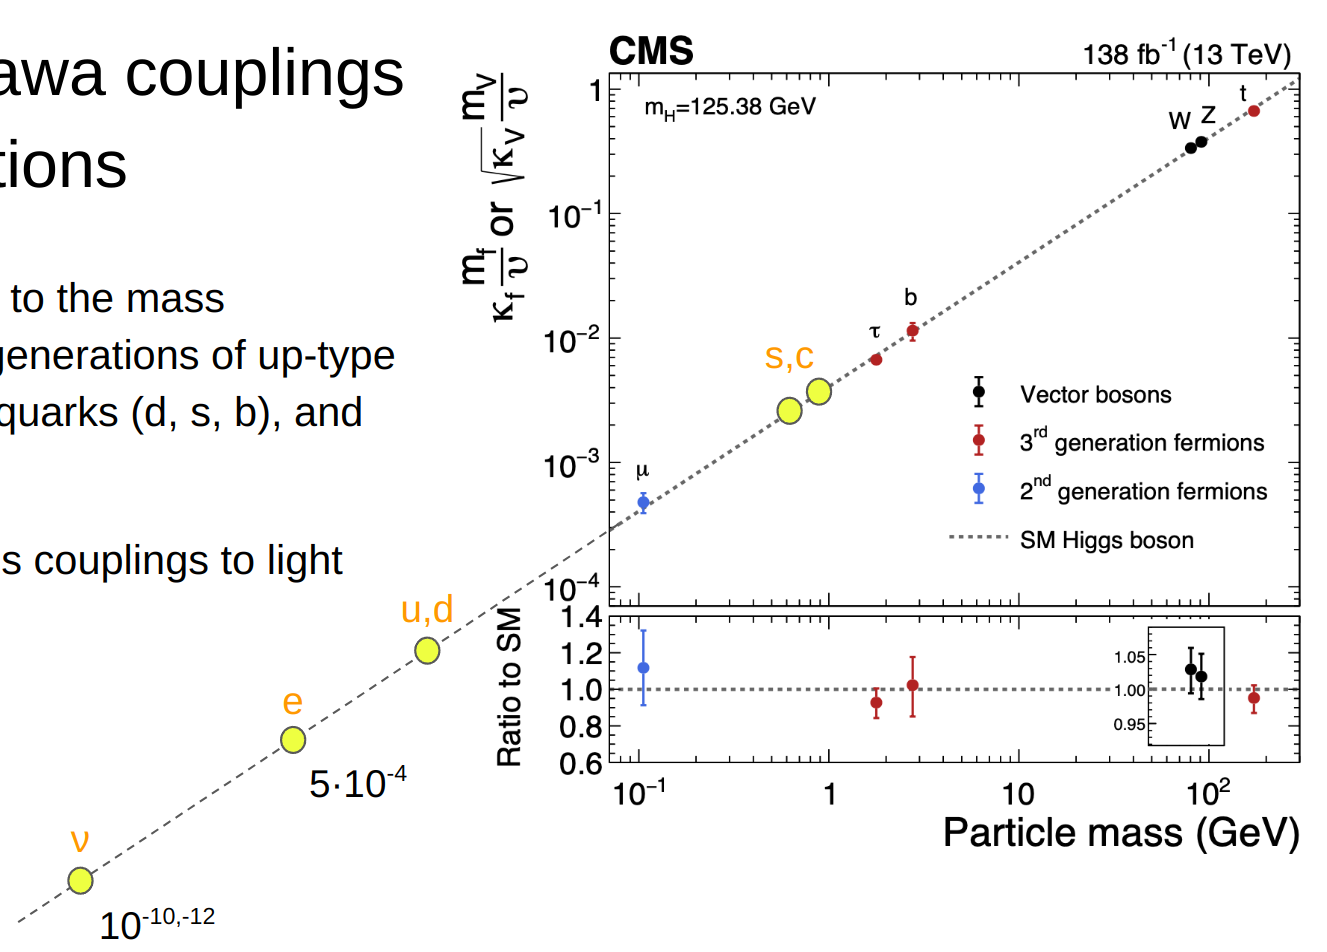
\includegraphics[width=0.60\mylength]{resources/Yukawa_couplings.png}
    \vspace*{-0.0cm}
    \caption{Relationship between the Yukawa couplings of the third-generation fermions, massive bosons, and the second-generation muon and its masses, from \cite{CMS:2022dwd}. The dashed straight line represents the Standard Model prediction.}
    \label{fig:Yukawa_couplings}
    \vspace*{-0.0cm}
\end{figure}

As of the time of writing, the measured values for the massive weak bosons, the third generation of fermions (top and bottom quarks and the tau lepton), as well as the second-generation lepton (the muon), align remarkably well with the Standard Model predictions, as seen in Figure \ref{fig:Yukawa_couplings}. This exceptional agreement with the predictions of the Higgs mechanism, spanning three orders of magnitude in mass, is a powerful test of the validity of the underlying physics.

To further test the validity of the SM, it is interesting to expand the plot to include lighter fermions, specifically the second-generation strange and charm quarks, as well as all first-generation fermions, including the up and down quarks and the electron. Additionally, the non-vanishing masses of the neutrinos may suggest a Yukawa-type coupling for them as well.

Direct searches for Higgs boson decays into charm pairs have been conducted by both the ATLAS and CMS collaborations. Additionally, searches for H$\decaysto e^+e^-$ have been carried out to complete the picture. Furthermore, both collaborations have explored potential Beyond the Standard Model (BSM) couplings of the Higgs boson, including searches for flavour-changing neutral currents via $t$-quark decays ($t\decaysto cH$ and $t\decaysto uH$), as well as lepton flavour-violating decays such as H$\decaysto e^\pm\mu^\mp$, H$\decaysto e^\pm\tau^\mp$ and H$\decaysto \mu^\pm\tau^\mp$. To date, no evidence supporting these couplings has been found.

Currently, the couplings of light quarks (u, d, s) to the Higgs boson remain loosely constrained by the existing data on the total Higgs boson width. The large multi-jet background at the LHC inhibits the study of such couplings with inclusive H$\decaysto q\bar{q}$. Rare exclusive decays of the Higgs boson into a light meson and a photon have been proposed as a probe of both flavor-conserving and flavor-violating couplings of the Higgs boson to light quarks (up, down, charm and strange). Exclusive decays involving $W^\pm$ and $Z^0$ bosons are also a possibility \cite{Kagan:2014ila}.

Initial experimental upper limits on hadronic two-body Higgs decays have been established by the ATLAS and CMS collaborations (ATLAS-CMS: H$\decaysto J/\psi + \gamma$ \cite{ATLAS:2022rej, CMS:2018gcm}, ATLAS: H$\decaysto \rho,\phi,\omega,K^{*0} + \gamma$ \cite{ATLAS:2017gko, ATLAS:2023alf}, CMS: H$\decaysto J/\psi,\rho,\phi + Z^0$ \cite{CMS:2022fsq, CMS:2020ggo}).

This analysis focuses on decays of the form H$\decaysto M\gamma$, where $M$ represents a light vector meson with a mass of approximately 1-2 GeV. It is important to note that, given that the Higgs boson has spin 0 and the photon has spin 1, the meson $M$ must be a \textit{vector} meson to conserve total angular momentum.

Table \ref{tab:Higgs_rare_decays} presents exotic decays of this form. The first three rows involve similar processes in which the vector meson decays into a pair of lighter, charged scalar mesons. These processes are currently under analysis by a group within the CMS collaboration as of the writing of this document. However, our specific focus within this analysis lies in the lower half of the table, where the vector meson decay involves a pair of charged scalar mesons along with neutral particles, specifically either pions or photons.

\begin{table}[!ht]
    \centering
    \begin{tabular}[t]{|l|C{6.5cm}|}
    \hline
    \multicolumn{1}{|c|}{\cellcolor{lightgray}Higgs boson rare decay} & \cellcolor{lightgray} Coupling \\ \hline &\\[-19pt]
        %$\text{H}\decaysto \rho^{0}_{\pi\pi}\gamma$& up/down quark                      & ??\%\\[-6.4pt]
        \hspace*{-3.75mm}
        \begin{tikzpicture}
            \matrix(decay)[matrix of math nodes, nodes={anchor=west}, row sep=-2]{
            \text{H}\decaysto \rho^{0}\gamma&\\
                &[-0mm] \pi^+\pi^- \ {\scriptstyle(\sim100\%)}\\
            };
            \draw[-stealth]([xshift=3.1mm, yshift=0.7mm]decay-1-1.south)|-(decay-2-2);
        \end{tikzpicture} & \vspace*{-1.3cm} up/down quark \\[-16pt]
        %$\text{H}\decaysto \phi_{KK}\gamma$&  strange quark                             & ??\%\\[-6.4pt]
        \hspace*{-3.75mm}
        \begin{tikzpicture}
            \matrix(decay)[matrix of math nodes, nodes={anchor=west}, row sep=-2]{
            \text{H}\decaysto \phi\gamma&\\
                &[-0mm] K^+K^- \ {\scriptstyle(49.1\pm0.5\%)}\\
            };
            \draw[-stealth]([xshift=3.1mm, yshift=0.7mm]decay-1-1.south)|-(decay-2-2);
        \end{tikzpicture} & \vspace*{-1.3cm} strange quark \\[-16pt]
        %$\text{H}\decaysto K^{*0}_{K\pi}\gamma$& flavor-violating down/strange quark    & ??\%\\ \cdashline{1-3}
        \hspace*{-3.75mm}
        \begin{tikzpicture}
            \matrix(decay)[matrix of math nodes, nodes={anchor=west}, row sep=-2]{
            \text{H}\decaysto K^{*0}\gamma&\\
                &[-0mm] K^{\pm}\pi^{\mp} \ {\scriptstyle(\sim100\%)}\\
            };
            \draw[-stealth]([xshift=3.1mm, yshift=0.7mm]decay-1-1.south)|-(decay-2-2);
        \end{tikzpicture} & \vspace*{-1.3cm} flavor-violating down/strange quark \\[-8pt]\cdashline{1-2}&\\[-19pt]
        %$\text{H}\decaysto \phi_{\pi\pi\pi^0}\gamma$& strange quark                     & ??\%\\[-6.4pt]
        \hspace*{-3.75mm}
        \begin{tikzpicture}
            \matrix(decay)[matrix of math nodes, nodes={anchor=west}, row sep=-2]{
            \text{H}\decaysto \phi\gamma&\\
                &[-0mm] \pi^+\pi^-\pi^0 \ {\scriptstyle(15.4\pm0.4\%)}\\
            };
            \draw[-stealth]([xshift=3.1mm, yshift=0.7mm]decay-1-1.south)|-(decay-2-2);
        \end{tikzpicture} & \vspace*{-1.3cm} strange quark \\[-16pt]
        %$\text{H}\decaysto \omega_{\pi\pi\pi^0}\gamma$& up/down quark                   & ??\%\\[-6.4pt]
        \hspace*{-3.75mm}
        \begin{tikzpicture}
            \matrix(decay)[matrix of math nodes, nodes={anchor=west}, row sep=-2]{
            \text{H}\decaysto \omega\gamma&\\
                &[-0mm] \pi^+\pi^-\pi^0 \ {\scriptstyle(89.2\pm0.7\%)}\\
            };
            \draw[-stealth]([xshift=3.1mm, yshift=0.7mm]decay-1-1.south)|-(decay-2-2);
        \end{tikzpicture} & \vspace*{-1.3cm} up/down quark  \\[-16pt]
        %$\text{H}\decaysto D^{*0}\gamma$& flavor-violating up/charm quark               & \\[-6.4pt]
        %$D^{*0}\decaysto D^0 + \pi^{0}/\gamma$&                                  &$100$\%            \\
        %$D^0\decaysto K^{-}\pi^{+}$&                                             &$3.947\pm0.030$\%  \\
        %$D^0\decaysto K^{-}\pi^{+}\pi^{0}$&                                      &$14.4\pm0.5$\%     \\\hline
        %$\text{H}\decaysto D^{*0}\gamma$& flavor-violating up/charm quark               & \\\hline
        \hspace*{-3.75mm}
        \begin{tikzpicture}
            \matrix(decay)[matrix of math nodes, nodes={anchor=west}, row sep=-2]{
            \text{H}\decaysto D^{*0}\gamma&\\
                &[-0mm] D^0 + \pi^{0}/\gamma \ {\scriptstyle(\sim100\%)}\\
                & &[-20mm] K^{-}\pi^{+} \ {\scriptstyle(3.95\pm0.03\%)}\\
                & & K^{-}\pi^{+}\pi^{0} \ {\scriptstyle(14.4\pm0.5\%)}\\
            };
            \draw[-stealth]([xshift=3mm, yshift=1mm]decay-1-1.south)|-(decay-2-2);
            \draw[-stealth]([xshift=-13mm, yshift=1mm]decay-2-2.south)|-(decay-3-3);
            \draw[-stealth]([xshift=-14mm, yshift=1mm]decay-2-2.south)|-(decay-4-3);
        \end{tikzpicture} & \vspace*{-2.47cm} flavor-violating up/charm quark \\[-8pt]\hline
        %$D^0\decaysto K^{S}\pi^{+}\pi^{-}$& Br$\sim2.8$\%\\\hline
    \end{tabular}
    \caption{Higgs rare decays of the form H$\protect\decaysto M\gamma$, where $M$ is a vector meson containing light quarks. The top half of the table focuses on decays where the light neutral vector meson decays into a pair of charged mesons. The bottom half of the table focuses on similar decays, but where there are also one or two neutral particles involved in the decay of the primary meson. All these decays are currently being analised by a group within the CMS collaboration.}
    \label{tab:Higgs_rare_decays}
\end{table}

The current branching ratio information of these decays that is known at the moment of this writing, both theoretical and experimental, is shown in Table \ref{tab:Higgs_rare_decays_values}.

\todo{Finish and comment comparison between SM branching rations and measured upper limits.}

\begin{table}[!ht]
    \centering
    \begin{tabular}{|l|cc|cc|}
        \hline
        \multicolumn{1}{|c|}{\cellcolor{lightgray}Decay channel} & \multicolumn{2}{c|}{\cellcolor{lightgray} SM $\mathcal{B}$} & \multicolumn{2}{c|}{\cellcolor{lightgray} Measured $\mathcal{B}$} \\ \hline
        $\text{H}\decaysto \rho^0\gamma$    & $(1.68 \pm 0.08)\times 10^{-5}$    & \cite{Konig:2015qat} & $< 8.8 \times 10^{-4}$ & \cite{ATLAS:2017gko}  \\
        $\text{H}\decaysto \phi\gamma$      & $(2.31 \pm 0.11)\times 10^{-6}$    & \cite{Konig:2015qat} & $< 4.8 \times 10^{-4}$ & \cite{ATLAS:2017gko}  \\
        $\text{H}\decaysto \omega\gamma$    & $(1.48 \pm 0.08)\times 10^{-6}$    & \cite{Konig:2015qat} & $< 1.5 \times 10^{-4}$ & \cite{ATLAS:2023alf}  \\
        $\text{H}\decaysto K^{*0}\gamma$    & \r LOOK UP & \r [??]              & $< 8.9 \times 10^{-5}$ & \cite{ATLAS:2023alf}  \\
        $\text{H}\decaysto D^{*0}\gamma$    & \r LOOK UP & \r [??]              & \r LOOK UP & \r [??]  \\ \hline
    \end{tabular}
    \caption{Higgs rare decay branching fractions. Because of the very large hadronic background at the LHC, only upper limits on the branching ratios have been computed so far, which are around two orders of magnitude bigger than the SM prediction.}
    \label{tab:Higgs_rare_decays_values}
\end{table}

When studying Higgs boson decays of the form H$\decaysto M\gamma$, which in essence are H$\decaysto q\bar{q}\gamma$, there are different Feynman diagrams that contribute to the width. We can distinguish the contributions into two different vertices. On the one hand, we have the tree-level diagram, which provides the direct contribution and is shown in diagram (a) of Figure \ref{fig:Higgs_rare_decay_veritces}. On the other hand, we have all other higher-order diagrams joined as an effective indirect vertex, represented in diagram (b) of Figure \ref{fig:Higgs_rare_decay_veritces}.

\begin{figure}[!ht]
    \captionsetup[subfigure]{labelformat=empty}
    \vspace*{-0.2cm}
    \centering
    \setlength{\mylength}{\textwidth}
    \begin{subfigure}[t]{0.5\mylength}
            \centering
            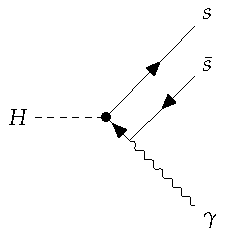
\includegraphics[height=0.26\mylength]{resources/H_rare_decays_vertices/v1.pdf}
            \setlength{\unitlength}{0.26\mylength}
            \caption{\footnotesize (a)}
    \end{subfigure}%
    \begin{subfigure}[t]{0.5\mylength}
            \centering
            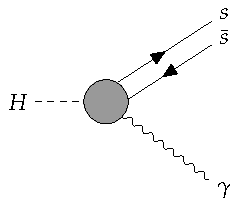
\includegraphics[height=0.26\mylength]{resources/H_rare_decays_vertices/v2_2.pdf}
            \setlength{\unitlength}{0.26\mylength}
            \caption{\footnotesize (b)}
    \end{subfigure}%
    \vspace*{-0.0cm}
    \caption{Direct (a) and indirect (b) contributions involved in the decays under analysis. Here we have considered the decay to a strange-antistrange quark pair, but it is analogous for the other light quarks.}
    \label{fig:Higgs_rare_decay_veritces}
    \vspace*{-0.0cm}
\end{figure}

According to the Standard Model, the direct contribution is of the order of $10^{-11}$, while the indirect contribution is of the order of $10^{-6}$, which means that higher-order corrections dominate the behaviour of these type of decays.

A few examples of diagrams that contribute to the effective vertex are provided in Figure \ref{fig:Higgs_decays_indirect}. In diagram (a) the blue loop can either be a heavy charged fermion loop or a $W^{\pm}$ boson loop.

\begin{figure}[!ht]
    \captionsetup[subfigure]{labelformat=empty}
    \vspace*{-0.2cm}
    \centering
    \setlength{\mylength}{\textwidth}
    \begin{subfigure}[t]{0.3546\mylength}
            \centering
            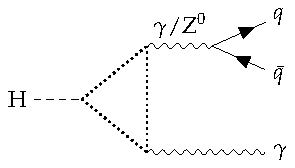
\includegraphics[width=0.344\mylength]{resources/H_rare_indirect/v1.pdf}
            \caption{\footnotesize (a)}
    \end{subfigure}%\begin{subfigure}[t]{0.5\mylength}
    \begin{subfigure}[t]{0.3546\mylength}
            \centering
            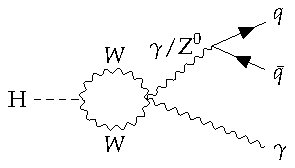
\includegraphics[width=0.344\mylength]{resources/H_rare_indirect/v2.pdf}
            \caption{\footnotesize (b)}
    \end{subfigure}%\begin{subfigure}[t]{0.5\mylength}
    \begin{subfigure}[t]{0.2907\mylength}
            \centering
            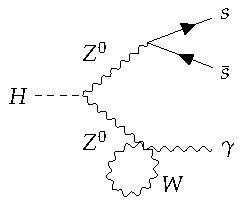
\includegraphics[width=0.282\mylength]{resources/H_rare_indirect/v3.pdf}
            \caption{\footnotesize (c)}
    \end{subfigure}%\begin{subfigure}[t]{0.5\mylength}
    %\begin{subfigure}[t]{0.5\mylength}
    %        \centering
    %        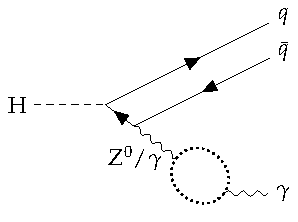
\includegraphics[height=0.26429\mylength]{resources/H_rare_indirect/v4.pdf}
    %        \caption{\footnotesize (d)}
    %\end{subfigure}%\begin{subfigure}[t]{0.5\mylength}
    %\vspace*{-0.0cm}
    \caption{Some examples of the many one-loop diagrams accounted for in the effective vertex. The blue loops are heavy charged fermion or $W^{\pm}$ boson loops.}
    \label{fig:Higgs_decays_indirect}
    \vspace*{-0.0cm}
\end{figure}

To ultimately compute the Yukawa couplings to the lighter families of quarks, one has to take into consideration contributions from both the direct and the indirect vertex, since experimentally what is measured from the direct decay is the overall effect coming from both vertices.

Therefore, the full diagrams of the decays that are object of study in these thesis (bottom half part of Table \ref{tab:Higgs_rare_decays}) are shown in Figure \ref{fig:Higgs_decays_studied}.

\begin{figure}[!ht]
    \captionsetup[subfigure]{labelformat=empty}
    \vspace*{-0.2cm}
    \centering
    \setlength{\mylength}{\textwidth}
    \begin{subfigure}[t]{0.43\mylength}
            \centering
            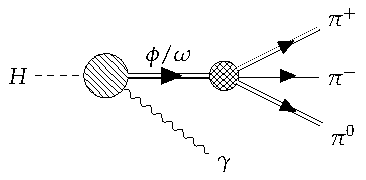
\includegraphics[width=0.41764\mylength]{resources/H_rare_decays_diagrams/v1.pdf}%62mm
            \caption{\footnotesize (a)}
    \end{subfigure}%\begin{subfigure}[t]{0.5\mylength}
    \begin{subfigure}[t]{0.57\mylength}
            \centering
            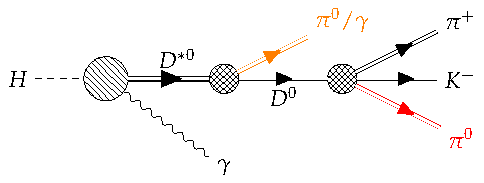
\includegraphics[width=0.55236\mylength]{resources/H_rare_decays_diagrams/v2_1.pdf}%82mm
            \caption{\footnotesize (b)}
    \end{subfigure}%\begin{subfigure}[t]{0.5\mylength}
    \caption{Full diagrams of the Higgs rare decays studied. Diagram (a) shows the decays $\text{H}\protect\decaysto \phi/\omega\gamma$. Diagram (b) shows the different decays $\text{H}\protect\decaysto D^{*0}\gamma$, where the orange line indicates that the particle can either be a $\pi^{0}$ ($\sim$ 65\%) or a $\gamma$ ($\sim$ 35\%) \cite{PDG}. This last diagram includes the two decays involving $D^{*0}$ studied, where $\pi^{0}$ is not there for the 2-body decay of the $D^{0}$ meson.}
    \label{fig:Higgs_decays_studied}
    \vspace*{-0.0cm}
\end{figure}

Diagram \ref{fig:Higgs_decays_studied} (a) depicts the decays $\text{H}\decaysto \phi\gamma$ and $\text{H}\decaysto \omega\gamma$, which are very similar and are going to share a lot of the features of the framework built. Diagram \ref{fig:Higgs_decays_studied} (b) shows the decays involving a $D^{*0}$ meson, $\text{H}\decaysto D^{*0}\gamma$, where the orange line from the decay of the $D^{*0}$ meson indicates that the particle can either be a $\pi^{0}$ (in around 65\% of the cases) or a $\gamma$ ($\sim$ 35\%) \cite{PDG}. This diagram encompasses the two decays involving $D^{*0}$ studied, where $D^{0}\decaysto K^{-}\pi^{+}$ corresponds to the diagram where the red line associated to $\pi^{0}$ is removed, and $D^{0}\decaysto K^{-}\pi^{+}\pi^{0}$ where the red edge is maintained.

The main difference between this analysis and the one studying the three decays presented in the top half of Table \ref{tab:Higgs_rare_decays} lies in the fact that we are dealing with 3-body decays involving neutral particles, which are more challenging to track compared to charged ones. That is why we will focus most of our attention on accurately recovering the missing neutral particles.

The main goal of this Master's Thesis is to compute a reasonable expected upper limit for the branching ratio of the aforementioned Higgs boson decays. Table \ref{tab:Higgs_rare_decays_values} shows the order of magnitude of the branching fractions one would ultimately like to measure. Nevertheless, due to the large hadronic background at the LHC, analyses of this kind are targeting an upper limit rather than a precise measurement at this stage.

Deviations from the predictions of the Standard Model within the Higgs boson sector can serve as compelling indications of new physics beyond our current understanding of particle physics. The Higgs boson plays a central role in the SM by giving particles mass through the Higgs mechanism. Therefore, any discrepancies in its properties, including decay widths, could reveal hidden phenomena and particles that the SM fails to describe.

One possible scenario involves determining an upper limit on a Higgs decay branching ratio that significantly exceeds the SM prediction. Such a discrepancy would suggest the presence of additional particles and interaction processes not accounted for in the SM. These new BSM particles could contribute to the Higgs decay width in ways not initially anticipated.

Accurate measurements are essential in this context, as they allow us to probe the Higgs sector with the highest level of precision. Through the precise determination of the Higgs boson's properties, one can identify even the most subtle deviations from the SM, providing clues about the nature of new physics. Consequently, the need for precision in Higgs boson measurements is of utmost importance, as it can not only further confirm the validity of the SM but also has the potential to illuminate the path towards a more comprehensive theory of particle physics, one that goes beyond the boundaries of the Standard Model.

The Future Circular Collider (FCC) project, with its proposed scenarios, including FCC-ee (electron-positron collisions) and FCC-hh (hadron-hadron collisions), presents a promising opportunity to advance our understanding of the Higgs boson and, by extension, the Standard Model \cite{FCC:2018byv}. The FCC-ee, with its high-energy lepton collisions, would enable us to conduct precise measurements of the Higgs boson's properties, including its interactions with other SM particles. This collider could provide an order of magnitude improvement in accuracy compared to current experiments, allowing for detailed studies of the Higgs, $W^\pm$, and $Z^0$ bosons, as well as the top quark \cite{Ellis:2015sca, dEnterria:2016fpc}. Together with the FCC-hh, which would operate with hadron collisions at significantly higher energies (potentially up to 30 times that of the current LHC \cite{FCC:2018vvp}), these colliders within the FCC project hold the potential to shed light on dark matter, probe neutrino masses, and investigate other unexplained phenomena.

\chapter[The CMS at the LHC]{The CMS at the LHC}

This chapter will provide an overview of the European Organization for Nuclear Research, commonly known by its acronym CERN (Conseil Européen pour la Recherche Nucléaire), along with the Large Hadron Collider (LHC) and the Compact Muon Solenoid (CMS) experiment. It will go through the most significant breakthroughs at CERN, with a particular emphasis on the discovery of the Higgs boson at the LHC in 2012 by the CMS and ATLAS collaborations \cite{CMS:2012qbp,ATLAS:2012yve}.

\section{The Large Hadron Collider at CERN}

The European Organization for Nuclear Research (CERN) is an intergovernmental organization composed of 23 member states that operates the world's largest particle physics laboratory. Established in 1954, CERN is situated on the Franco-Swiss border near Geneva, Switzerland, and is one of the largest and most influential research organizations in particle physics. The missions of CERN include world-class research in fundamental physics, sustainable and environmentally responsible accelerator facilities, global collaboration in science and technology advancement and the education and engagement of future scientists, engineers and the broader public.

CERN has been home to many accelerators, including the original linear accelerator Linac1 (in operation from 1959 until 1992), the Linac2 (1978 - 2018), the Super Proton-Antiproton Synchrotron (S$p\bar{p}$S) (1981-1991), the Large Electron-Positron Collider (LEP) (1989-2000), and the current Large Hadron Collider (LHC), which was constructed between 1998 and 2008 and achieved its first collisions in 2010. The Future Circular Collider (FCC) is proposed to be the successor of LHC at CERN \cite{FCC:2018byv}.

During its nearly 70-year history since its creation, many important achievements in particle physics have been made through experiments at CERN, including:
\begin{itemize}
    \setlength\itemsep{0em}
    \item The discovery of neutral currents by studying neutrinos produced by the PS/SPS neutrino beam interacting in the Gargamelle bubble chamber in 1973 \cite{GargamelleNeutrino:1973jyy}.
    \item The discovery of the $W^\pm$ and $Z^0$ bosons in the UA1 and UA2 experiments in 1983 \cite{UA1:1983crd, UA2:1983tsx}.
    \item The determination of the number of light neutrino families at LEP in 1989 \cite{ALEPH:1989kcj}.
    \item The discovery of direct CP violation in the NA48 experiment in 1999 \cite{NA48:1999szy}.
    \item The discovery of the Higgs boson at LHC by the CMS and ATLAS collaborations in 2012 \cite{CMS:2012qbp,ATLAS:2012yve}.
\end{itemize}

Today, the main particle accelerator at CERN is the LHC. The Large Hadron Collider (LHC) is a hadron collider primarily used for proton-proton collisions but also capable of heavy-ion collisions. It was designed to investigate the properties of the Standard Model, in particular the Higgs boson, and to study the physics Beyond the Standard Model by analysing discrepancies in the SM or via direct searches of particles. It has a circumference of 26.659 kilometers and is located underground at depths ranging from 50 to 175 meters, making it the world's largest and highest-energy particle collider \cite{Evans:2008zzb, CERN:Facts_figures}.

\begin{figure}[!ht]
    \vspace*{-0.0cm}
    \centering
    \setlength{\mylength}{\textwidth}
    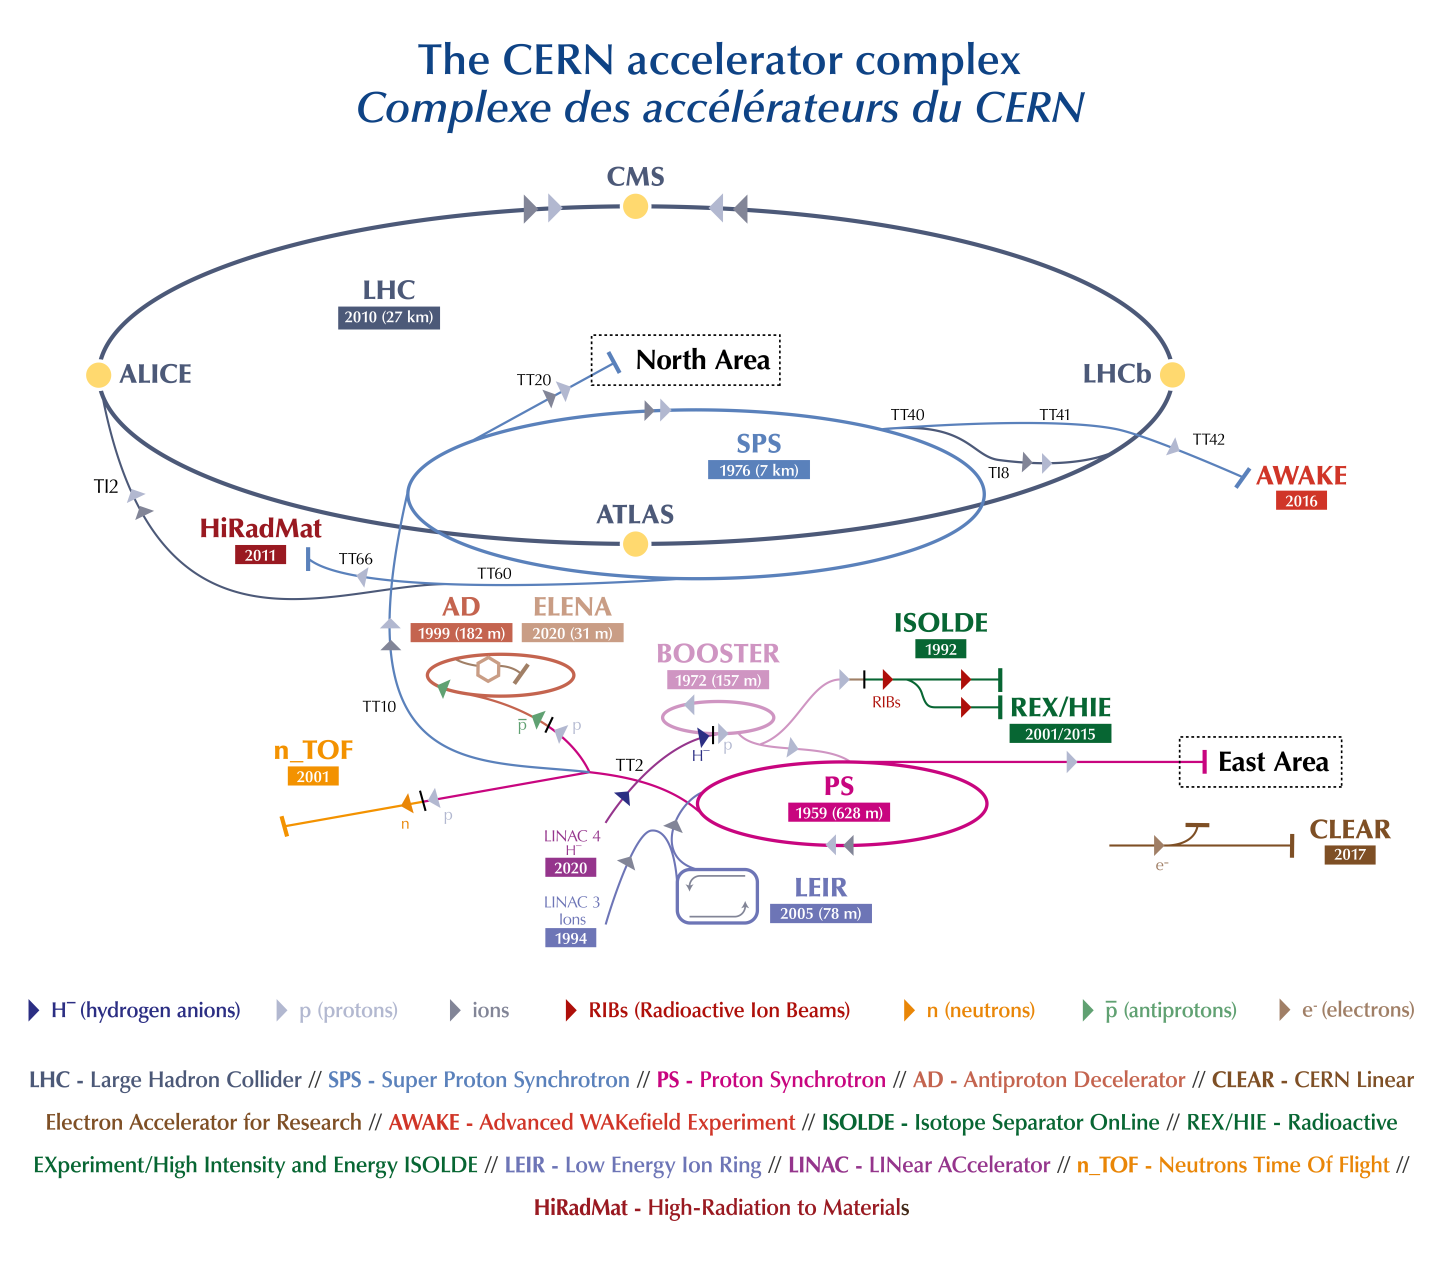
\includegraphics[width=0.84\mylength]{resources/LHC.png}
    \vspace*{-0.0cm}
    \caption{The CERN accelerator complex. The four main experiments can be seen in four different points around the LHC. Source: \cite{Mobs:2684277}.}
    \label{fig:CERN_LHC}
    \vspace*{-0.3cm}
\end{figure}

Two beams circulate in opposite directions within the LHC, guided by 9593 superconducting magnets. Operating at a center-of-mass energy of $\sqrt{s} = 13\ \TeV$, protons from each beam have an energy of 6.5 TeV and complete about 11245 orbits around the collider's circumference every second. This is achieved by initially stripping hydrogen atoms of their electrons, leaving the protons. Several accelerators are used in sequence to accelerate these protons: first, Linac2 (Linac4 after 2020) accelerates them to 50 MeV, followed by the Proton Synchrotron Booster (PSB) accelerating them further to 1.4 GeV, the Proton Synchrotron (PS) to 25 GeV, and finally, the Super Proton Synchrotron (SPS), where they reach 450 GeV. The beams are then injected into the LHC, which takes them to 6.5 TeV using superconducting dipole magnets, cooled to 1.9 K with superfluid helium, producing a magnetic field of 8.3 T, and eight radio frequency (RF) cavities per beam. By tuning the energy of the protons that have a different timing than that of the RF cavity, the phase oscillations of the electromagnetic fields within these RF cavities divide the protons into 2808 bunches, each containing about $1.15\times10^{11}$ protons. The collisions resulting from this process occur approximately every 25 ns, equivalent to a frequency of 40 MHz. These collisions take place at four interaction points, where the four major LHC experiments are located: ATLAS (A Toroidal LHC ApparatuS) \cite{ATLAS:1994vge}, CMS (Compact Muon Solenoid) \cite{CMS:1994hea}, ALICE (A Large Ion Collider Experiment) \cite{413235}, and LHCb (Large Hadron Collider beauty) \cite{LHCb:1998kcv}. Of these four experiments, ATLAS and CMS are multipurpose detectors designed to study a wide range of physics phenomena. ALICE is specifically conceived to record the collisions of ion beams, while LHCb is optimized for studying $b$-physics. Moreover, several smaller experiments at the LHC focus on more specific physics goals. Figure \ref{fig:CERN_LHC} shows a diagram of CERN's Accelerator Complex.

One of the main advantages of LHC being a proton-proton collider, rather than an electron-positron collider like its predecessor LEP, is that it suffers much less from the effects of synchrotron radiation. This effect causes charged accelerated particles to lose energy, inversely proportional to the fourth power of the particle mass, making proton-proton collisions more energy efficient for a 13 TeV regime.

During Run 1 of the LHC, which spanned from 2010 to 2012, the center-of-mass energy ranged from 7 to 8 TeV, and CMS recorded a total integrated luminosity of 29.45 fb$^{-1}$. Run 2 took place from 2015 to 2018, with an energy of 13 TeV, and a total integrated luminosity of 163.6 fb$^{-1}$. In 2022, Run 3 began and is scheduled to conclude in 2026, with an energy of 13.6 TeV. In the first year of Run 3, the total integrated luminosity reached 42 fb$^{-1}$, and is expected to be around 300 fb$^{-1}$ by the end of the Run \cite{CMS:luminosity}. The data that is going to be used in this analysis is from the CMS collaboration and was taken in 2018 (Run 2), with $\sqrt{s} = 13\ \TeV$ and an integrated luminosity of 39.5 fb$^{-1}$.

\section{The Compact Muon Solenoid}

One of the four large particle detectors at the LHC is the Compact Muon Solenoid (CMS) detector \cite{CMS:1994hea, CMS:2008xjf}. It is designed to optimize the muon detection system in proton-proton collisions, featuring a cylindrical geometry, measuring 21.5 m in length and 15 m in diameter, with a total weight of approximately 14000 tonnes. It is characterized by its solenoid magnet, which generates a 4 T magnetic field used to bend charged particles to measure their transverse momentum ($p_T$).

Concentric layers of detector subsystems surround the collision point of the particle beams at the center of the detector to measure particle trajectories and their properties. These subsystems, starting from the interaction point, include the silicon tracker, the electromagnetic calorimeter (ECAL), and the hadronic calorimeter (HCAL). Beyond the superconducting solenoid magnet there is another outer HCAL and the muon system, where another magnetic field of approximately 2 T bends the muons in the opposite direction of the first magnet. Each subdetector specializes in measuring certain particles, but they work together to reconstruct events. For more detailed information refer to \cite{CMS:2006myw}. A full diagram of the structure of CMS is shown in Figure \ref{fig:CMS_cutaway}, while a cross section is presented in Figure \ref{fig:CMS_slice}.

\begin{figure}[!ht]
    \vspace*{-0.0cm}
    \centering
    \setlength{\mylength}{\textwidth}
    \includegraphics[width=0.99\mylength]{resources/CMS_cutaway_labels.pdf}
    \vspace*{-0.0cm}
    \caption{A cutaway view of the CMS detector. Figure from \cite{Sakuma:2013jqa}.}
    \label{fig:CMS_cutaway}
    \vspace*{-0.3cm}
\end{figure}

\begin{figure}[!ht]
    \vspace*{-0.0cm}
    \centering
    \setlength{\mylength}{\textwidth}
    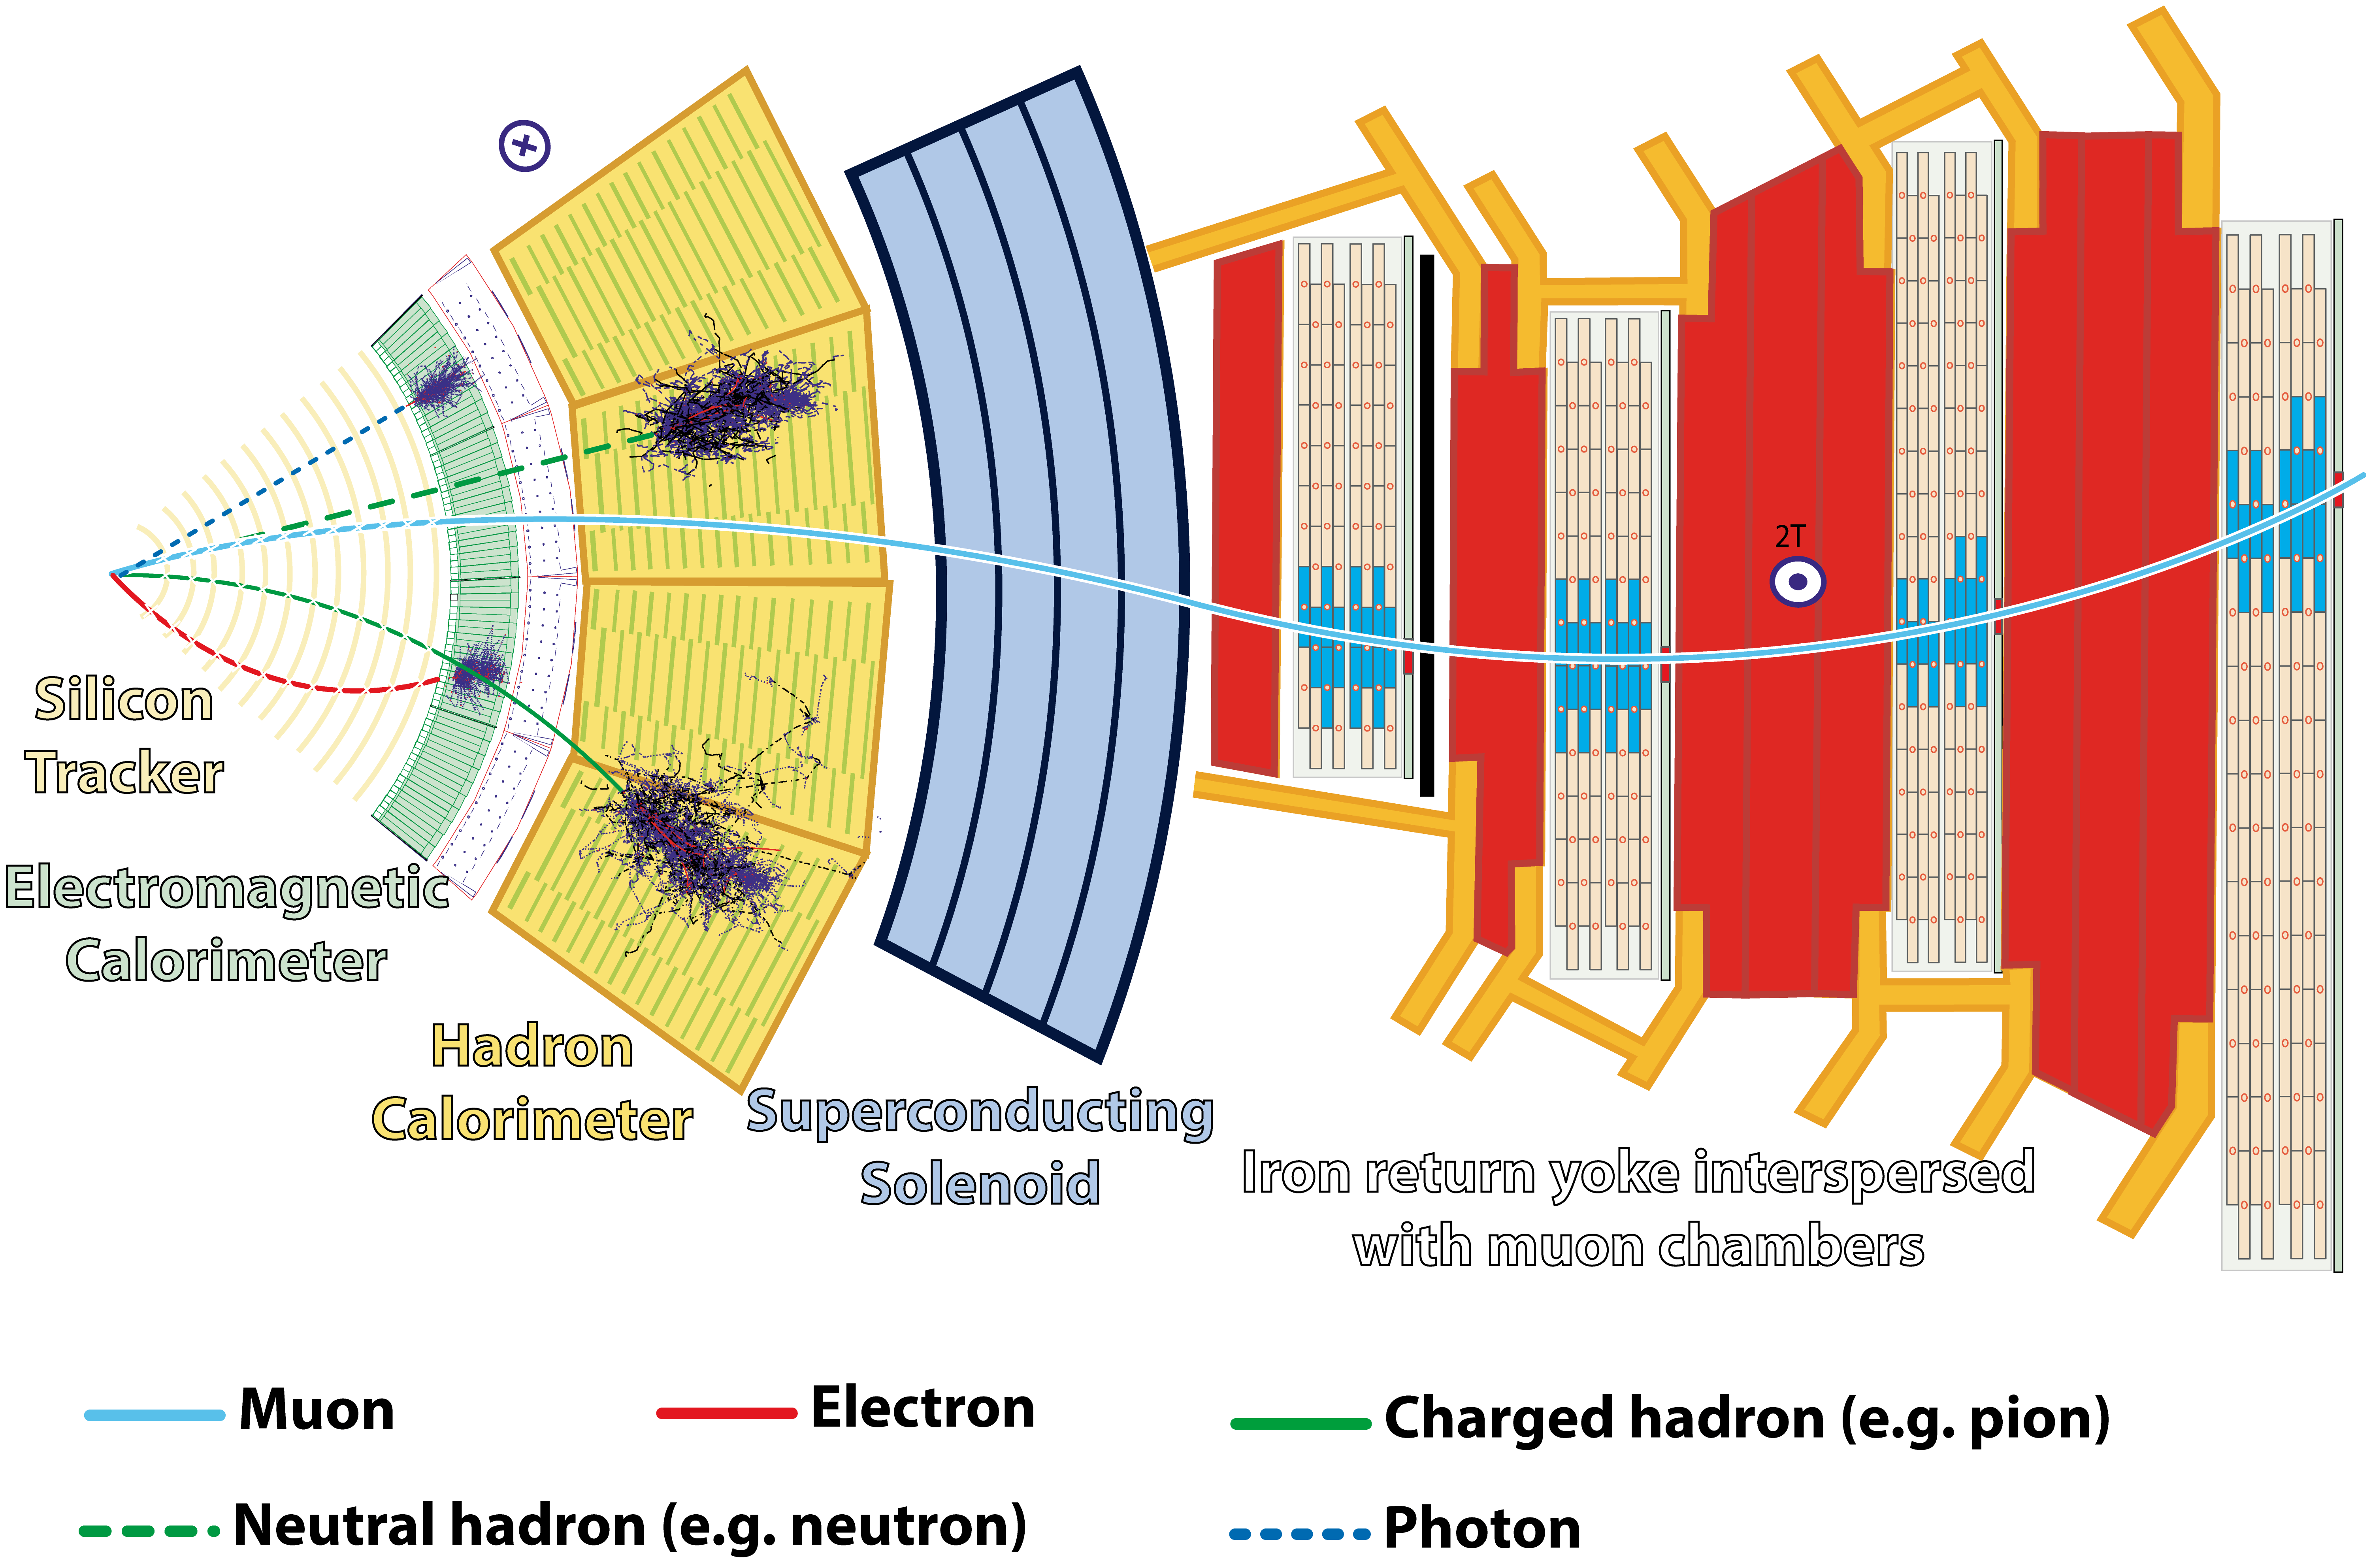
\includegraphics[width=0.85\mylength]{resources/CMS_slice.png}
    \vspace*{-0.0cm}
    \caption{A slice of the CMS detector, with an illustration of the behaviour of different particles. Figure from \cite{Barney:2120661}.}
    \label{fig:CMS_slice}
    \vspace*{-0.3cm}
\end{figure}

The coordinate system in CMS has its origin centered at the nominal collision point within the detector. The $z$-axis follows the beam line, the $y$-axis points vertically upward, and the $x$-axis points radially inward toward the center of the LHC ring. The azimuthal angle $\phi$ is measured from the $x$-axis in the $x-y$ plane, with the radial coordinate denoted as $r$, and the polar angle $\theta$ is measured from the $z$-axis. However, $\theta$ is not often used because it is not Lorentz invariant for boosts along the direction of the beam. Instead, the pseudorapidity is defined as $\eta = -\ln{\left(\tan{\frac{\theta}{2}}\right)}$, which is Lorentz invariant. From this, it is possible to define the momentum orthogonal to the beam direction, denoted as $p_T$.

The silicon tracker is designed to measure the trajectory, charge and momentum of charged particles traversing it, as well as to reconstruct secondary vertices. It comprises two types of silicon detectors: the pixel detector (inner tracker) and the silicon strip tracker (outer tracker). They operate by measuring the ionization of charged particles. When a charged particle traverses the doped silicon wafer, it creates electron-hole pairs that move toward collection electrodes due to an applied electric field. These pairs are organized into silicon strips or pixels, providing a two-dimensional measurement. Multiple silicon wafers are arranged in different layers, and the hits measured in each layer are used to reconstruct the tracks of charged particles through the detector. The pixel detector is the innermost component, consisting of four barrel layers and three endcap disks. The silicon strip tracker is positioned just outside, extending to a radius of 1.1 m and comprising 15148 strips arranged in ten barrel layers and twelve endcap disks.

The primary purpose of the electronic calorimiter (ECAL) is to measure the energy and direction of electrons, positrons and photons. It is constructed with homogeneous lead tungstate (PbWO$_4$) crystals that serve as both active scintillating material to detect the electromagnetic signal and absorbing material to initiate electromagnetic (EM) showers. Energy deposition is measured through crystal ionization, and their deexcitation photons are detected by dedicated photodetectors. The short radiation length of the crystals, $X_0 = 0.89$ cm, ensures that the EM showers remain confined within a small region. The photodetectors are designed to withstand the high radiation and high magnetic field environment while being sufficiently fast compared to the LHC bunch crossing time. The ECAL consists of main parts: the ECAL barrel (EB), covering $\abs{\eta} < 1.479$, composed of 61200 crystals and which uses avalanche photodiodes, and the ECAL endcaps (EE), covering $1.479 < \abs{\eta} < 3.0$, composed of 7324 crystals in each (lower granularity compared to the barrel) and which use vacuum phototriodes. To account for the reduced endcap granularity, preshower detectors are installed before the lead tungstate crystals, covering $1.653 < \abs{\eta} < 2.6$, intended for identifying neutral pions, distinguish electrons against minimum ionizing particles, and improve position measurements. This design enables the ECAL to completely stop electrons and photons emerging from the tracker, allowing for accurate energy measurement.

Four hadronic calorimeters (HCAL) are positioned outside the ECAL. They are designed to generate hadronic showers when strongly interacting particles pass through their absorption material. These particles interact in the absorber layers, producing numerous secondary particles and often showers, which are measured by the scintillators. The HCAL are bigger than the ECAL because the nuclear interaction length $\lambda_\text{int}$ is also larger than the electromagnetic radiation length $X_0$ (e.g., for iron, $\lambda_\text{int}=16.8$ cm, while $X_0=1.76$ cm \cite{Buckley:2021fcn}). The HCAL barrel (HB) rests between the ECAL and the magnet ($R=1.77-2.95$ m), covering $\abs{\eta} < 1.4$. The HCAL endcap (HE) covers $1.3 < \abs{\eta} < 3.0$. Both the HB and the HE are made of brass and plastic scintillators. The HCAL outer detector (HO) is placed outside the magnet in the barrel region ($\abs{\eta} < 1.26$) to catch the tail of the shower, and it is made of iron and plastic scintillators. To ensure optimal efficiency in different pseudorapidity ranges, there is a fourth HCAL placed in the endcap regions after the muon systems. The HCAL forward detector (HF) covers $3.0 < \abs{\eta} < 5.0$ at $\abs{z} = 11.2$ m, where it is subject to much higher radiation. It is distinguished from the other HCAL sections because it is built with steel and quartz fibers, leading to shorter hadronic showers for better absorption of very forward hadron showers. Note that the ECAL already absorbs a fraction of the energy of the hadrons, but the HCAL design allows it to fully stop the hadrons and measure any remaining energy, which is later combined with the ECAL information to obtain a complete picture.

Muon identification was a focal point for CMS because muons produced in proton-proton collisions offer clear lepton signatures for a wide range of physics processes and helps with their reconstruction. The CMS muon system consists of several subdetectors dedicated to measure muons with high precision. To achieve accurate muon identification, the muon detectors were designed with extensive pseudorapidity coverage, up to $\eta = 2.4$. CMS's muon system uses three types of detectors: Drift Tubes, Resistive Plate Chambers and Cathode Strip Chambers. Muon Drift Tubes (DT) contain a wire and a gas mixture (85\% Ar, 15\% CO$_2$) at atmospheric pressure that ionizes when traversed by a muon. The deexcitation electrons follow the electric field to reach the wire, recording the signal. By recording the distance from the wires and the location along the wires, the DTs determine two coordinates of the muon's positions. Resistive Plate Chambers (RPC) are gaseous (95.2\% C$_2$H$_2$F$_4$, 4.5\% i-C$_4$H$_{10}$, 0.3\% SF$_6$) parallel plate capacitors with high timing resolution. Cathode Strip Chambers (CSC) consist of positively charged anode wires crossed with negatively charged cathode panels within a gas volume (40\% Ar, 50\% CO$_2$, and 10\% CF$_4$), which ionize when traversed by a muon: positive ions move toward the cathode and the electrons move toward the anode wires. In the CMS detector's barrel ($\abs{\eta} < 1.2$), the DTs are arranged in four concentric layers interleaved with five layers of the iron magnet yoke and six layers of RPCs, as shown in Figure \ref{fig:CMS_slice}. In the endcap region, reaching $\eta = 2.4$, there are three RPC layers (up to $\eta = 1.6$) and six CSC layers, chosen in this region for their ability to resist high non-uniform magnetic fields. Muons do not deposit much energy in matter, so they pass through both calorimeters with most of their momentum. The muon chambers then provide further information about the muon's trajectory, as they are the only particles with a clear signal in this section. These trajectories, combined with those of the trackers, allow for better muon identification and provide additional data on their momenta.

Storing all recorded events in the detector is impractical, so only events meeting specific conditions are preserved. The Level 1 (L1) Trigger uses local trigger information from all subdetectors, excluding the Inner Tracker, to determine whether to save an event. With the aid of custom hardware and firmware, it reduces the event rate from 40 MHz to 100 kHz. It considers information from the four highest $E_T$ electrons, photons, central jets, forward jets, tau-jets, the four highest $p_T$ muons, the event's missing transverse energy (MET), and the scalar sum of the jet transverse momenta (HT). Subsequently, data is processed by the High-Level Trigger (HLT), a comparatively slower software, to further filter events based on trigger menus, reducing the rate to around 1 kHz. The CMS offline physics object reconstruction is achieved using the Particle Flow (PF) algorithm, which integrates information from all subdetectors to reconstruct all particles in the event.

The Compact Muon Solenoid experiment is one of the largest international scientific collaborations in history, involving more than 6000 particle physicists, engineers, technicians, students and support staff from 257 institutes in 59 countries as of October 2023 \cite{CERN:CMS_people}.

\section{The discovery of the Higgs boson at CMS}

\todo{Discovery of the higgs: when, CMS/ATLAS, which channels were used, sigmas, initial mass and values.}

\chapter[Analysis]{Analysis}\label{chap:analysis}

This chapter constitutes the core of this dissertation. Here, we will discuss the analysis conducted, starting with a general overview, followed by an explanation of the samples, triggers, and object definitions. We will then talk about the corrections applied to the data and simulations to enhance the analysis results. Additionally, we will cover the criteria used in event selection and how the signal and background have been modeled. Finally, we will present the expected upper limits of the branching ratio for each channel, as this analysis will only be working with simulated signal, alongside simulated and real background data. The chapter concludes by addressing the subsequent steps required before data unblinding and the attainment of the final experimental measurement, as well as suggesting other ideas to improve the results.

\section{Analysis overview}\label{sec:analysis_overview}

This analysis uses data from proton-proton collisions corresponding to an integrated luminosity of 39.54 fb$^{-1}$ at $\sqrt{s}=$13 TeV, collected by the CMS detector at LHC in 2018 during Run 2. It only targets the Higgs boson production mode via gluon fusion (ggH), which accounts for approximately 87\% of the Higgs boson production at LHC at $\sqrt{s}=$13 TeV. Although it is possible to extend this analysis to include more production modes, time constraints have led us to focus to the main production channel. The final states of interest consist of an isolated and energetic photon, a charged meson pair, and photons compatible with a third (and sometimes fourth) neutral meson, with 0 hadronic jets and no additional leptons ($e/\mu$). The mesons considered here are a $\phi$, a $\omega$ and a $D^{*0}$, each further decaying into two charged particles and a third (and fourth) neutral one (see Table \ref{tab:Higgs_rare_decays_three}).

\begin{table}[ht]
    \centering
    \begin{tabular}{ll}
        $\text{H}\decaysto \phi\gamma$ ,& $\phi\decaysto \pi^+\pi^-\pi^0$ \\
        $\text{H}\decaysto \omega\gamma$ ,& $\omega\decaysto \pi^+\pi^-\pi^0$\\
        $\text{H}\decaysto D^{*0}\gamma$ ,& $D^{*0}\decaysto D^{0}\pi^{0}/\gamma,\ D^{0}\decaysto K^{\mp}\pi^{\pm}$\\
        $\text{H}\decaysto D^{*0}\gamma$ ,& $D^{*0}\decaysto D^{0}\pi^{0}/\gamma,\ D^{0}\decaysto K^{\mp}\pi^{\pm}\pi^{0}$
    \end{tabular}
    \caption{Higgs rare decays under study in this analysis.}
    \label{tab:Higgs_rare_decays_three}
\end{table}

The analysis strategy involves categorizing events to increase the signal to background ratio. In our production mode (ggH), the largest background source in this analysis consists of $\gamma$ plus jets events.

The branching fractions of rare Higgs boson decays to a meson and photon can be computed using a factorization approach in QCD. The calculation considers both direct and indirect contributions, as explained in the first chapter and depicted in Figure \ref{fig:Higgs_rare_decay_veritces}. The interference between these components is significant. In the SM, the indirect component dominates, and the Higgs boson couplings to light quarks are probed by searching for modifications in this branching fraction due to interference effects.

As previously explained, given the exotic nature of the decays under study, the theoretical decay widths being so small, the large hadronic background at the LHC, and the limited amount of data collected, we cannot aim for precise measurements of the branching fractions. Instead, the end goal of this thesis is to calculate a reasonable upper limit on the branching ratio of the aforementioned Higgs boson decays, using Monte Carlo (MC) samples to model the SM expected signal. To obtain a competitive, real result, this initial estimation requires further refinement and improvement, such as considering additional background sources, systematic uncertainties, etc.

The main difference between this analysis and the study of the three decays in the upper half of Table \ref{tab:Higgs_rare_decays} is that, in contrast to those, we are studying 3-body decays with neutral particles, which are more challenging to track than charged ones. The framework used for this analysis builds upon the existing framework for the simpler two-body decays currently under analysis by the Particle Physics Collaboration at the Massachusetts Institute of Technology (MIT). To extend their study to include three-body decays involving neutral particles, our main focus has been on accurately recovering the missing neutral particles.

\section{Samples and triggers}\label{sec:samples_triggers}

To develop this analysis, the data file format used is one designed by CMS, which is an extended version of \verb+NANOAOD+. It is based on the official \verb+NANOAODv9+ recipe and includes the reconstructed mesons, as described in Section \ref{sec:objects}, as additional objects. The \verb+NANOAOD+ format consists of an Ntuple-like structure used by CMS, which can be read using bare root, and containing the per-event information that is needed in most generic analyses \cite{CMS:NanoAOD}. This analysis is performed using the \verb+ROOT+ data analysis framework, an open-source data analysis tool commonly used in high energy physics written mainly in C++ \cite{CERN:root}.

\subsection{Data and Tau trigger}\label{subsec:data_tau_trigger}

Events are selected from proton-proton collision data at a center-of-mass energy of $\sqrt{s}=$13 TeV and a bunch spacing of 25 ns, collected by the CMS experiment during the LHC's Run 2 in 2018, corresponding to a total integrated luminosity of 39.54 fb$^{-1}$. Good run ranges and luminosity blocks are chosen based on criteria encoded in a golden JSON file.

To filter data in the gluon fusion production mode, a tau-like trigger is employed. This Tau trigger selects a photon with $\pT^{\gamma} > 35\ \GeV$ and a ditrack system with $\pT^{\text{jet}} > 35\ \GeV$, after going through the L1 trigger, which also imposes rapidity restrictions of $\abs{\eta^{\gamma}}<2.1$ and $\abs{\eta^{\text{jet}}}<2.1$. The trigger is applied to both data and MC. Introduced in 2018, this trigger recorded events enriched in gluon fusion production of the Higgs boson and VBF that were not registered by the dedicated trigger, providing an effective luminosity of 39.54 fb$^{-1}$. The trigger selecting events during 2018 is encoded as \verb+Photon35_TwoProngs35+. \todo{Should I include trigger efficiencies for each channel in the appendix? If so, how do I obtain these plots?} The datasets used in gluon fusion and VBF analysis are detailed in Table \ref{tab:ggH_datasets}.

\begin{table}[ht]
    \centering
    \begin{tabular}{|c|c|c|}
        \hline
        \multicolumn{1}{|c|}{\cellcolor{lightgray}Year} & \cellcolor{lightgray}Dataset & \cellcolor{lightgray}Integrated luminosity [fb$^{-1}$] \\ \hline
        2018    & \verb+/Tau/Run2018B-UL2018+  & 0.67 \\
        2018    & \verb+/Tau/Run2018C-UL2018+  & 6.94 \\
        2018    & \verb+/Tau/Run2018D-UL2018+  & 31.93 \\ \hline
    \end{tabular}
    \caption{Datasets used in the gluon fusion analysis from the campaign MiniAODv2 of the MINIAOD data tier.}
    \label{tab:ggH_datasets}
\end{table}

\subsection{Background simulation}

The background estimation will ultimately rely solely on data. However, at the early stage of this analysis, simulated samples are used to understand the background processes affecting the different selected final states. The main background process for the gluon fusion production mode is a single photon and jets.

Every event is generated at leading order (LO) precision using the MADGRAPH5 generator \verb+MG5_aMC@NLO+ \cite{Alwall:2014hca} and POWHEG \cite{Alioli:2010xd}, while PYTHIA8 \cite{Sjostrand:2014zea} is used for the hadronization. For all simulations, the NNPDF 3.1 \cite{NNPDF:2017mvq} next-to-next-to-leading-order (NNLO) parton distribution functions (PDFs) are used, while the modeling of the underlying event is generated using the CMS Pythia 5 (CP5) tunes \cite{CMS:2019csb}. The Run 2 legacy reconstruction algorithms \cite{Elmetenawee:2020emw} are used for all the MC and data samples. The campaign and global tag used to produce the background and signal MC samples are \verb+RunIISummer20UL18MiniAODv2-106X+ and \verb+upgrade2018_realistic_v16_L1v1+, respectively. Table \ref{tab:MC_samples} summarizes the list of datasets used for the study along with their cross sections \cite{CERN:xsdb}.

\begin{table}[ht]
    \centering
    \begin{tabular}{|l|c|}
        \hline
        \multicolumn{1}{|c|}{\cellcolor{lightgray}Monte Carlo name} & \cellcolor{lightgray}Cross section [pb] \\ \hline
        \verb+GJets_HT-40To100_TuneCP5_13TeV-madgraphMLM-pythia8+  & 18540 (LO) $\times$ 1.26 \\
        \verb+GJets_HT-100To200_TuneCP5_13TeV-madgraphMLM-pythia8+  & 8644 (LO) $\times$ 1.26 \\
        \verb+GJets_HT-200To400_TuneCP5_13TeV-madgraphMLM-pythia8+  & 2183 (LO) $\times$ 1.26 \\
        \verb+GJets_HT-400To600_TuneCP5_13TeV-madgraphMLM-pythia8+  & 260.2 (LO) $\times$ 1.26 \\
        \verb+GJets_HT-600ToInf_TuneCP5_13TeV-madgraphMLM-pythia8+  & 86.58 (LO) $\times$ 1.26 \\ \hline
    \end{tabular}
    \caption{MC samples used for the gluon fusion production mode. The normalization of $\gamma+$jets is scaled by 1.26 \cite{CMS:2018qao} \todo{WHY?}.}
    \label{tab:MC_samples}
\end{table}

\subsection{Signal simulation}

The only Higgs boson production mode studied, gluon fusion, is generated at next-to-leading order (NLO) using the POWHEGv2 event generator extended with the MiNLO procedure \cite{Hamilton:2012np}. The production rates and kinematic distributions for the Higgs boson with $m_H=125\ \GeV$ are assumed throughout. In particular, the cross section for gluon fusion is computed at NNLO in QCD and NLO in electroweak accuracy, resulting in 48.58 pb, as provided by the LHC Higgs Cross Section Working Group in Ref. \cite{LHCHiggsCrossSectionWorkingGroup:2016ypw}.

The decay of the Higgs boson is handled by Pythia, and it does not simulate direct and indirect effective vertices. The expected SM branching fractions of the Higgs rare decays are as previously shown in Table \ref{tab:Higgs_rare_decays_values}: $\mathcal{B}(\text{H}\decaysto \phi\gamma) = (2.31 \pm 0.11)\times 10^{-6}$ and $\mathcal{B}(\text{H}\decaysto \omega\gamma) = (1.48 \pm 0.08)\times 10^{-6}$, while $\mathcal{B}(\text{H}\decaysto D^{*0}\gamma)$ has not yet been computed. In the analysis, however, the branching ratios are set to
\begin{equation*}
    \mathcal{B}(\text{H}\decaysto \phi\gamma) = \mathcal{B}(\text{H}\decaysto \omega\gamma) = \mathcal{B}(\text{H}\decaysto D^{*0}\gamma) = 1\ .
\end{equation*}
This is because then, when computing a limit, the obtained value is directly the measured upper limit of the branching ratio itself. If we were to set the branching fractions to the SM values, the measured quantities would be the signal strengths, i.e., the factors by which the observed fractions exceed the SM values. The branching fractions of the meson decays used are also shown in Table \ref{tab:Higgs_rare_decays}, but further detailed in Table \ref{tab:Meson_decay_br}.

\begin{table}[!ht]
    \centering
    \begin{tabular}{|l|c|}
        \hline
        \multicolumn{1}{|c|}{\cellcolor{lightgray}Meson decay channel} & \multicolumn{1}{c|}{\cellcolor{lightgray} SM $\mathcal{B}$ (\%)} \\ \hline
        $\phi\decaysto \pi^+\pi^-\pi^0$     & $15.4 \pm 0.4$   \\
        $\omega\decaysto \pi^+\pi^-\pi^0$   & $89.2 \pm 0.7$   \\
        $D^{*0}\decaysto D^{0}\pi^0$        & $64.7 \pm 0.9$   \\
        $D^{*0}\decaysto D^{0}\gamma$       & $35.3 \pm 0.9$   \\
        $D^{0}\decaysto K^{\mp}\pi^{\pm}$           & $3.962 \pm 0.031$   \\
        $D^{0}\decaysto K^{\mp}\pi^{\pm}\pi^0$      & $14.43 \pm 0.50$   \\
        \hline
    \end{tabular}
    \caption{Meson decay branching ratios used throughout the analysis, from the PDG \cite{PDG}.}
    \label{tab:Meson_decay_br}
\end{table}

\section{Object definitions}\label{sec:objects}

This analysis primarily relies on photons and charged tracks to extract the final state signature of exclusive hadronic decays, while also making use of other physics objects such as additional leptons (or the lack thereof) and hadronic jets to suppress background. All used objects, except the mesons, are discussed in this section, with the next section dedicated solely to meson reconstruction.
\vspace*{-6pt}
\begin{myitemlist}
    \item[Primary vertex (PV):] To consider an event, it must contain at least one primary vertex, which is regarded as the vertex of the hard interaction. There should be a minimum of four tracks associated with the selected primary vertex (from the Higgs boson, the photon and the ditrack system). For events with multiple selected vertices, the PV is chosen to be the vertex corresponding to the hardest scattering in the event, determined using tracking information alone, as described in Ref. \cite{Contardo:2015bmq}.

    \item[Jets:] During the reconstruction of a proton-proton (pp) collision, jets are often reconstructed with a $\pT$ that differs from that of the final-state particles within the jet. The jet energy corrections (JEC) adjust the reconstructed jet energy to match the true energy of the final-state particles. The CMS collaboration has developed a factorized approach to these JEC, consisting of multiple levels that correct various physics or detector effects. This approach provides flexibility in the corrections to suit various types of analyses. These correction levels are commonly referred to as L1FastJet, L2Relative, L3Absolute, and L2L3Residual.

    The flow of these JEC is as follows: jets are reconstructed from particle flow (PF) candidates using the anti-$k_\text{T}$ clustering algorithm with a distance parameter of $R = 0.4$ as implemented by FastJet \cite{Cacciari:2011ma}. Jets within this small cone (referred to as AK4 jets for $R = 0.4$) are selected among those with $\pT > 20\ \GeV$ and $\abs{\eta} < 4.7$ for forward tagging. At the LHC, a significant number of pp collisions occur simultaniously during one bunch crossing, with soft ones contaminating the collision of interest. To mitigate this effect, known as \textit{pileup} (PU), charged hadrons not originating from the primary vertex are removed using the charged hadron subtraction (CHS) algorithm \cite{CMS:2014ata, Perloff:2012wpa}. The tight pileup ID criterion is applied to reduce the contamination of jets with $\pT < 50\ \GeV$ initiated by the pileup interactions. Jets are corrected for the response inside the detector, differentially in $\abs{\eta} - \abs{\phi}$, for the pileup contributions, and for data only, the residual difference observed between data and simulation.
    
    In the current analysis version, the \verb+Summer19UL+ jet energy corrections set is used, as well as the DeepJet tagging algorithm with the medium working point to identify $b$-jets \cite{Bols:2020bkb}.

    \item[Missing energy:] The $\pT^{\text{miss}}$ measures the transverse momentum imbalance in the event. To estimate it, the deepMET algorithm \cite{Feng:2744871} is used, and $\pT^{\text{miss}}$ filters are then applied to account for instrumental noise in the detector and minimize the impact of the non-collisional background.
    
    \item[Photons:] Photon candidates are reconstructed as SuperCluster objects in the ECAL with $\ET > 38\ \GeV$ and $\abs{\eta^{\gamma}} < 2.1$ in both the barrel and endcap regions. In addition, photons have to satisfy the multivariate analysis (MVA) based selection identification (mvaID) criteria following the \verb+Fall17IsoV2+ recipe \cite{CMS:2020uim}. For the production mode used, the mvaID provides 80\% (90\%) signal selection efficiency for the endcap (barrel) region. The mvaID criteria include photon isolation, charged hadron isolation, and require photons to pass shower shape preselection cuts \cite{Rembser:2019ijh}. The photon's ECAL cluster must be inconsistent with charged particle tracks reconstructed in the silicon tracker to reject electrons faking photons, achieved using a conversion safe electron veto. Residual $\ET$ -dependent photon energy scale and smearing corrections are applied. Additional photons with looser requirements ($\ET > 20\ \GeV$ and the WP90 version of the photonID) are also vetoed to reduce the potential contribution of diphotons. Table \ref{tab:photon_selection} summarizes the criteria for photon selection.

    \begin{table}[!ht]
        \centering
        \begin{tabular}{|l|c|}
            \hline
                \multicolumn{2}{|c|}{\cellcolor{lightgray}Selection criteria ($\gamma$ from PV)}\\ \hline
                $\pT^{\gamma}$            &$>38$ GeV\\
                $\abs{\eta^{\gamma}}$       &$<2.1$ \\
                mvaID                       &WP90/WP80 \\
                electron Veto               &Yes \\\hline
            \end{tabular}
        \caption{Selection criteria applied to the photon from the primary vertex.}
        \label{tab:photon_selection}
    \end{table}

    An additional correction was attempted, involving shifting the photon's origin to that of the PV of the meson. This slight adjustment to the initial coordinates led to a minor change in the four-momentum variables of the photon, but it did not consistently reduce the discrepancy with the generation-level particle values. Consequently, it was discarded and not used.

\end{myitemlist}

\section{Meson reconstruction \todo{ADD FOURTH D0* CHANNEL}}\label{sec:meson_reconstruction}

The $\phi$, $\omega$ and $D^{*0}$ mesons decay products are reconstructed using charged particle tracks measured in the tracker, as well as energy deposited in the ECAL compatible with neutral particles coming also from the PV. For the $\phi$ and $\omega$ mesons, the targeted charged ditrack is $\pi^\pm\pi^\mp$, while for the $D^{*0}$ meson the charged ditrack is $K^{\mp}\pi^{\pm}$.

In the following sections, the term \textit{ditrack system} will refer to the system of the two charged tracks, and even though they not form a real particle, notions like ditrack mass will be used (understand the mass of the ditrack as the mass component of the sum of the four-momenta of both tracks). To refer to the meson originating from the PV, namely $\phi$, $\omega$ and $D^{*0}$, terms like \textit{meson} or \textit{full meson} will be used, emphasizing that the neutral particles have been accounted for. Some considerations have been made to precisely reconstruct the full meson:
\vspace*{-6pt}
\begin{myitemlist}
    \item[Track selection:] To be selected, the tracks need to satisfy a ``high purity'' reconstruction criteria, which considers the number of tracker layers with hits, track fit quality, and the impact parameter values relative to their uncertainties. For a detailed description of the algorithm, refer to Ref. \cite{CMS:2014pgm}.

    \item[Meson decay vertex:] The meson decay vertex is determined using the standard CMSSW \cite{CMSSW} kinematic vertex fitting package, as described in Ref. \cite{Prokofiev:2005zz}. Using the candidate's decay vertex and its associated momentum, a newly fitted transient track is constructed to represent the meson candidate. Then, for each primary vertex, the track is extrapolated to the nearest point in 3D space. The meson vertex's longitudinal distance is required to be within 24 cm from the center of the detector.
    
    \item[Isolation:] To ensure good track selection, a dedicated isolation criterion of the candidate based on the tracks is used. This dimensionless isolation parameter (Iso) is determined from the meson's momentum and other tracks within a cone of radius $\Delta R = 0.3$ around the ditrack system's direction. Only tracks with $\pT > 0.9\ \GeV$ associated with the same meson vertex are considered, excluding the charged-hadron candidates that define the ditrack. The definition is as follows:
    \begin{equation*}
        \text{Iso} = \frac{\pT^{\text{meson}}}{\pT^{\text{meson}}+\sum_{\text{trk}}{\abs{\pT^{\text{trk}}}}}
    \end{equation*}
    A high isolation value will be required to consider a meson candidate (over 0.9).

    \item[Neutral particle photons:] For each selected ditrack, up to two photons with $\pT > 5 \ \GeV$ are recovered in a small cone of $\Delta R = 0.05$ around the ditrack direction. These photons account for the recovery of neutral particles, as $\pi^{0}\decaysto\gamma\gamma$ in $\sim 98.8\%$ with $c\tau=25$ nm \cite{PDG}. From generation-level MC we know that photons coming from neutral particle decays that in turn come from the three-body decays must be very collimated with the ditrack system. In the case of the $\phi$/$\omega$ channels and the $D^{*0}$ channel when $D^{0}$ decays into three bodies, these photons directly originate from the $\pi^0$ of the three-body decay. In the case of the $D^{*0}$ channel, the photon comes either directly from $D^{*0}\decaysto D^{0}\gamma$ or from de decay of the $\pi^0$ from $D^{*0}\decaysto D^{0}\pi^0$.
    
    \item[Ditrack mass hypothesis:] The invariant mass of the refitted ditrack system is also used to reduce contamination from background events. The mass of the pair, assuming the charged-pion hypothesis for the two tracks, is consistent with the charged components of the $\phi$ and $\omega$ mesons. Since the ditrack system is not a real resonance, its mass is very wide but consistent and useful for reducing background events. In the case of the $D^{*0}$ channel, two scenarios are considered. On the one hand, when $D^{0}$ decays into a pair of charged particles (kaon-pion) the ditrack system's invariant mass is a real narrow resonance (namely $D^{0}$) coherent with the mass of that meson. On the other hand, when $D^{0}$ decays into a pair of charged particles and a neutral pion, one finds the same scenario as for the $\phi$/$\omega$ decay channels.
    
    The exact used selection criteria will be presented at the end of this section, but it is worth noting that for the $\phi$/$\omega$ three-body decays involving a $\pi^0$, the mass of the ditrack is approximately two-thirds of the full meson's mass (each pion carries roughly a third of the energy).

    Furthermore, instead of recovering the ditrack invariant mass by only retrieving the mass component of the sum of both four-momenta, the CMSSW kinematic fit has been employed. To study the performance of this fit, it is useful to define the \textit{residual} as the difference between the reconstructed values and the corresponding generation-level ones. Figure \ref{fig:kinematic_fit_residuals} displays the residual of the ditrack invariant mass reconstruction with and without the kinematic fits with vertex constraint for every decay mode.
    \begin{figure}[!ht]
        \captionsetup[subfigure]{labelformat=empty}
        \vspace*{-0.2cm}
        \centering
        \setlength{\mylength}{\textwidth}
        \begin{subfigure}[t]{0.50\mylength}
                \centering
                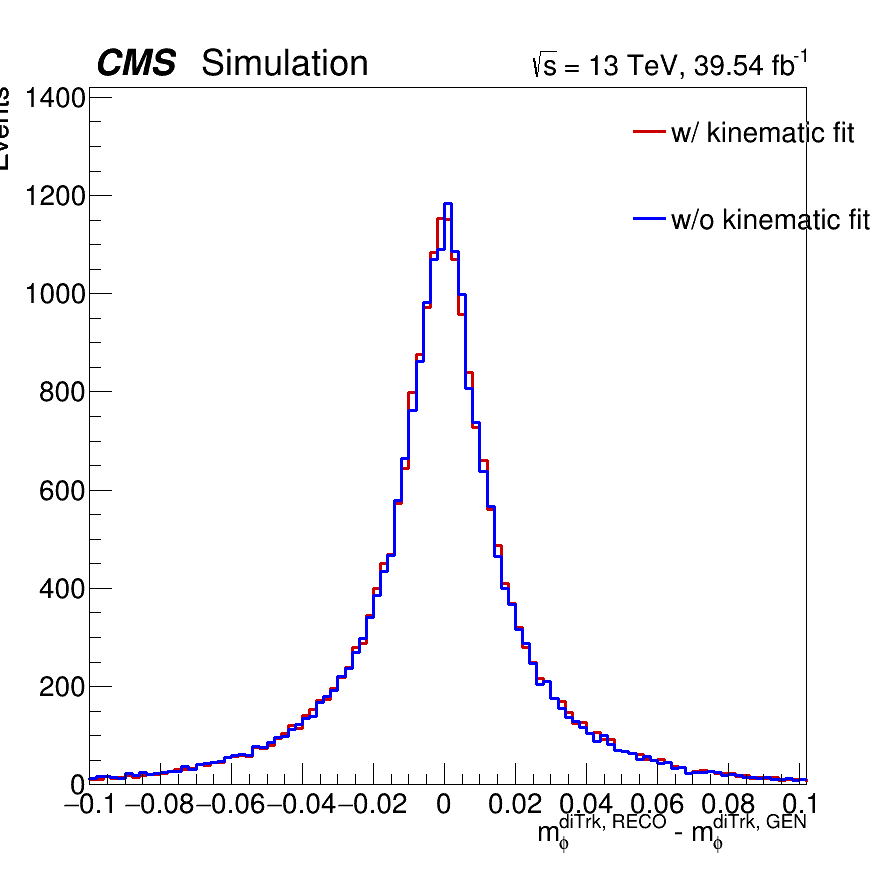
\includegraphics[width=0.45\mylength]{resources/plots/Phi3_kinematic_fit_residual.png}
                \caption{\footnotesize (a)}
        \end{subfigure}%
        \begin{subfigure}[t]{0.50\mylength}
                \centering
                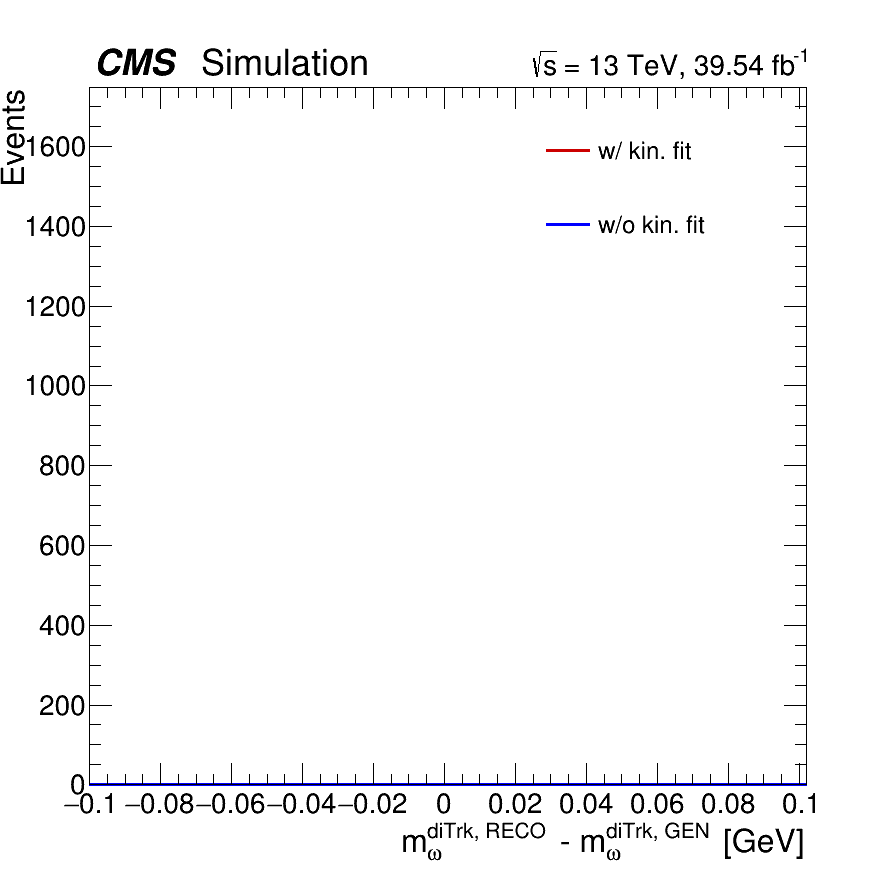
\includegraphics[width=0.45\mylength]{resources/plots/Omega_kinematic_fit_residual.png}
                \caption{\footnotesize (b)}
        \end{subfigure}%\begin{subfigure}[t]{0.50\mylength}\baselineskip
        \vskip\baselineskip
        \vspace*{-0.1cm}
        \begin{subfigure}[t]{0.50\mylength}
                \centering
                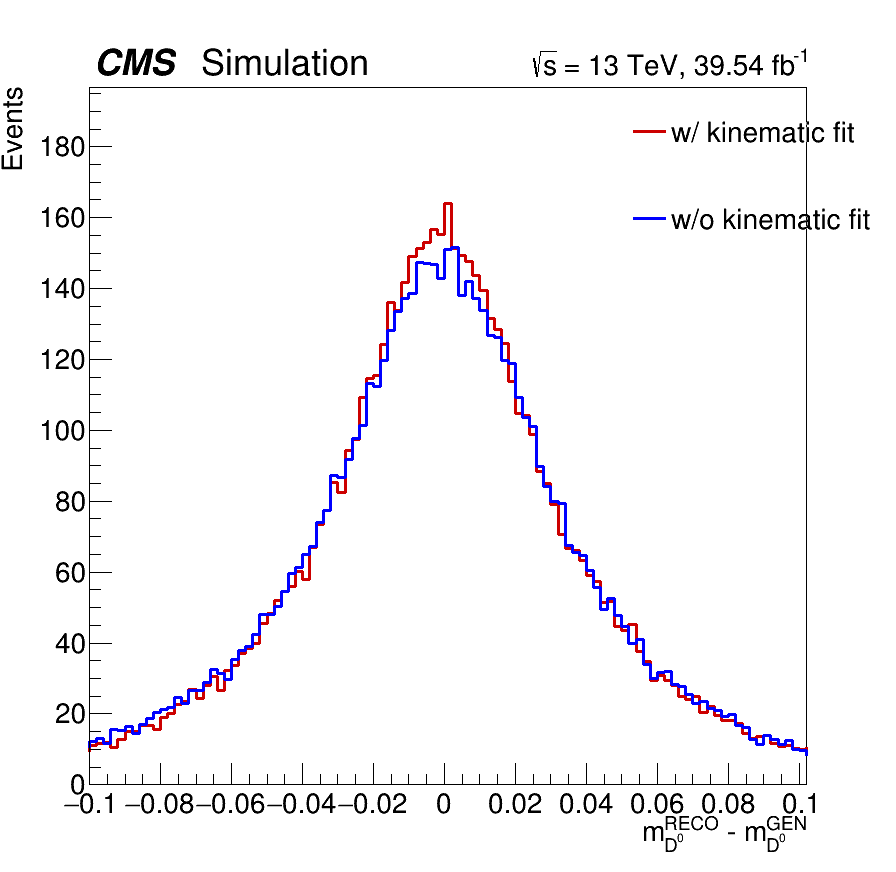
\includegraphics[width=0.45\mylength]{resources/plots/D0Star_2body_kinematic_fit_residual.png}
                \caption{\footnotesize (c)}
        \end{subfigure}%\begin{subfigure}[t]{0.50\mylength}
        \begin{subfigure}[t]{0.50\mylength}
                \centering
                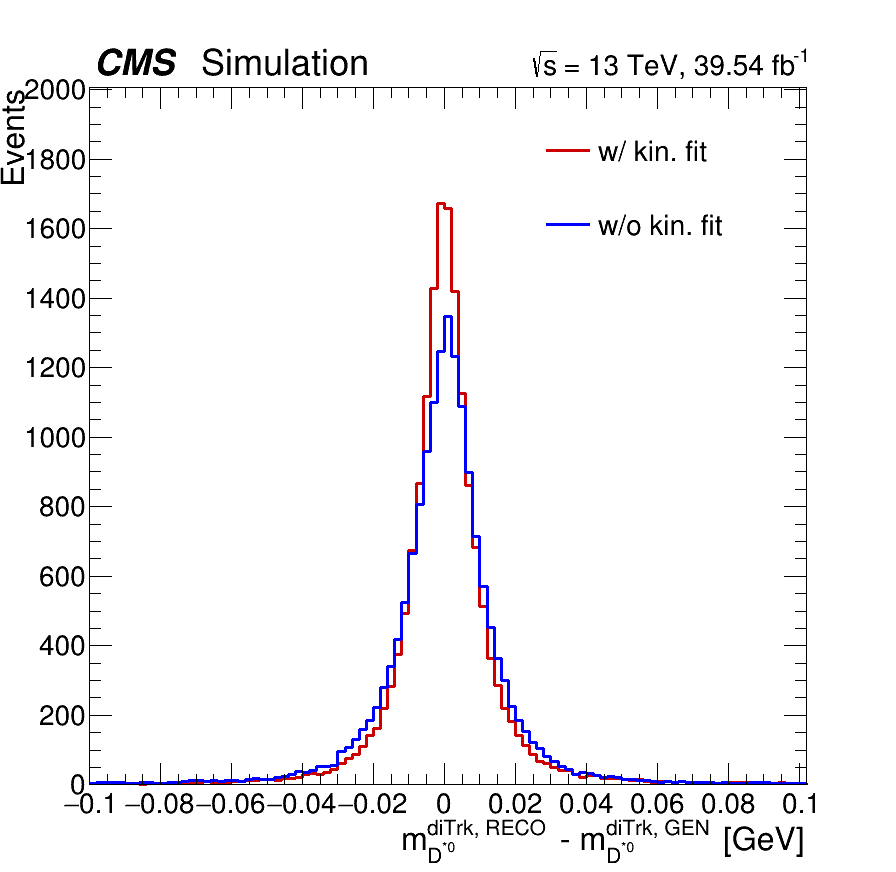
\includegraphics[width=0.45\mylength]{resources/plots/D0Star_3body_kinematic_fit_residual.png}
                \caption{\footnotesize (d)}
        \end{subfigure}%
        \vspace*{-0.0cm}
        \caption{Ditrack mass residuals for the different decay channels. (a) is for $\phi$, (b) is for $\omega$, (c) is for $D^{*0}$ 2-body, and (d) is for $D^{*0}$ 3-body.}
        \label{fig:kinematic_fit_residuals}
        \vspace*{-0.0cm}
    \end{figure}
    Table \ref{tab:kinematic_fit_RMSE} shows the root mean squared errors with respect to generation-level, both with and without the kinematic fit, for each channel. Applying the kinematic fit improves the reconstructed ditrack invariant mass values for all channels.

    \begin{table}[!ht]
        \centering
        \begin{tabular}{|l|c|C{2.9cm}@{}c|}
            \hline
            \cellcolor{lightgray}Decay channel & \cellcolor{lightgray}RMSE without kinematic fit & \multicolumn{2}{c|}{\cellcolor{lightgray}RMSE with kinematic fit} \\ \hline
            $\phi$          &37.8 MeV   &34.0 MeV  & (-10\%)   \\
            \r$\omega$        &\r xx.x MeV   & x\r x.x MeV &\r (-x\%)  \\
            $D^{*0}$ 2-body &49.7 MeV   &47.6 MeV  & (-4\%)     \\
            $D^{*0}$ 3-body &73.3 MeV   &55.5 MeV  & (-24\%)    \\
            \hline
            \end{tabular}
        \caption{Root mean squared errors (RMSE) with and without the kinematic fit for each decay mode.}
        \label{tab:kinematic_fit_RMSE}
    \end{table}
    
    \item[Meson mass hypothesis:] The simplest way to reconstruct the four-momentum of the full meson is by summing the four-momenta of the ditrack system and those from the photons compatible with the decay of neutral particles. This approach was initially used for all channels. Nevertheless, for the $\phi$, $\omega$ and $D^{*0}$ 3-body decay channels, additional corrections were applied.
    
    Consider that the photons in the $\Delta R$ cone come from the $\pi^{0}\decaysto\gamma\gamma$ decay. When only one photon is recovered, it means that either both photons ended up in the same ECAL crystal, or that one of them was too soft to be measured ($\pT < 5\ \GeV$) and therefore only one is detected. Following the first hypothesis, we can interpret the energy deposited in the same ECAL cell as the energy from the full pion. To account for this, whenever only one photon is recovered, we assign this object a non-zero mass (the pion's mass) before adding the four-momenta. This correction is of very low energy, and thus the changes in $\pT$, $\eta$ or $\phi$ of the full meson are imperceptible, but its mass is visibly affected. Figure \ref{fig:full_meson_mass_residuals} and Table \ref{tab:full_meson_mass_residuals_RMSE} show the residual of the full meson invariant mass reconstruction and the RMSE, respectively, with and without the $\pi^0$ mass correction for the $\phi$ and $\omega$ decay modes.
    \begin{figure}[!ht]
        \captionsetup[subfigure]{labelformat=empty}
        \vspace*{-0.2cm}
        \centering
        \setlength{\mylength}{\textwidth}
        \begin{subfigure}[t]{0.50\mylength}
                \centering
                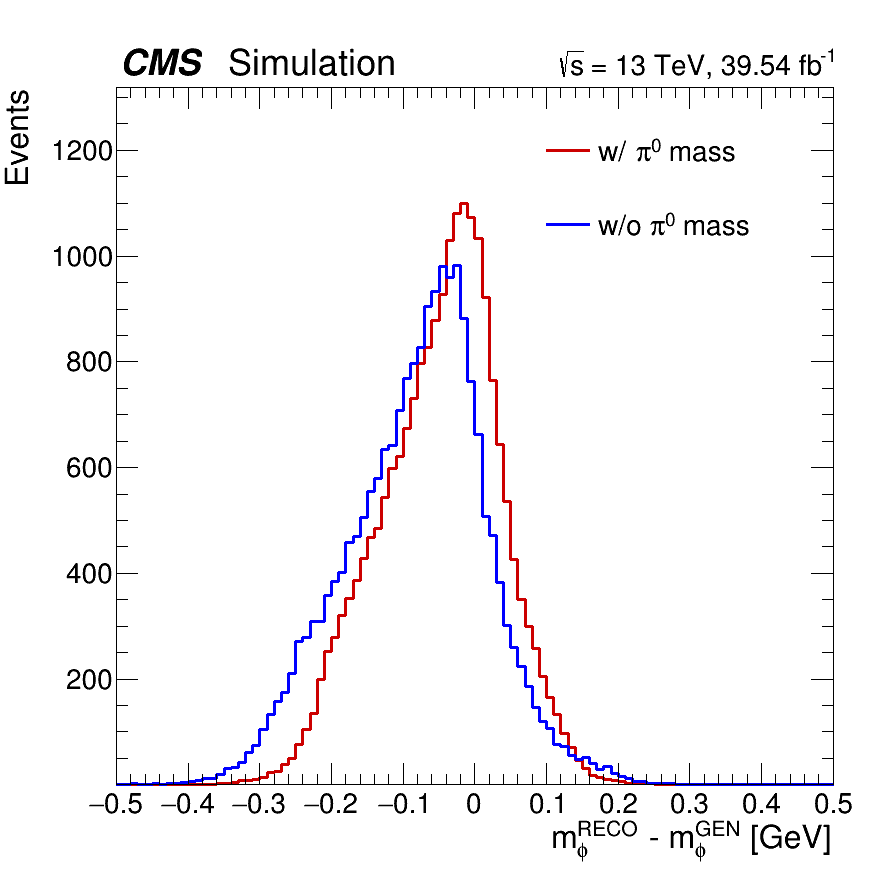
\includegraphics[width=0.45\mylength]{resources/plots/Phi3_fullmeson_mass_residual.png}
                \caption{\footnotesize (a)}
        \end{subfigure}%
        \begin{subfigure}[t]{0.50\mylength}
                \centering
                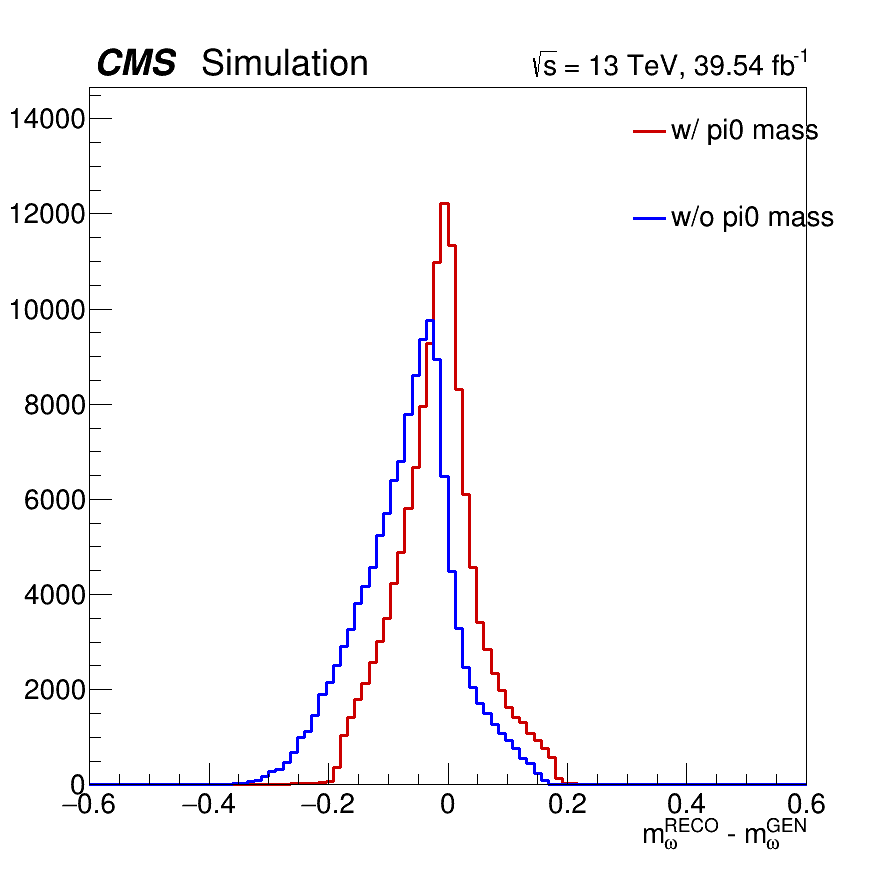
\includegraphics[width=0.45\mylength]{resources/plots/Omega_fullmeson_mass_residual.png}
                \caption{\footnotesize (b)}
        \end{subfigure}%\begin{subfigure}[t]{0.50\mylength}\baselineski
        \caption{Full meson mass residuals for the different decay channels. (a) is for $\phi$, (b) is for $\omega$.}
        \label{fig:full_meson_mass_residuals}
        \vspace*{-0.0cm}
    \end{figure}

    This slight improvement will enable us to narrow some selection cuts and reduce more background events, ultimately improving the final result.

    \begin{table}[!ht]
        \centering
        \begin{tabular}{|l|c|C{3.2cm}@{}c|}
            \hline
            \cellcolor{lightgray}Decay channel & \cellcolor{lightgray}RMSE without $m_{\pi^0}$ correction& \multicolumn{2}{c|}{\cellcolor{lightgray}RMSE with $m_{\pi^0}$ correction} \\ \hline
            $\phi$          &130.2 MeV   &117.7 MeV  & (-10\%)   \\
            $\omega$        &127.9 MeV   &113.1 MeV  & (-12\%)   \\
            \hline
            \end{tabular}
        \caption{Root mean squared errors with and without the $m_{\pi^0}$ correction for the $\phi$ and $\omega$ decay modes.}
        \label{tab:full_meson_mass_residuals_RMSE}
    \end{table}

    An additional correction was attempted. The idea was to reconstruct the neutral particle by summing the recovered photons, and then forcing the reconstructed neutral particle to have the $\pi^0$'s mass while maintaining the energy and direction ($\eta$ and $\phi$) unchanged. This required a slight modification of the neutral particle's transverse momenta, as given by
    \begin{equation*}
        \pT = \sqrt{(E^2 - m^2)(1-\tanh^2\eta)}\ .
    \end{equation*}
    When adding this neutral particle to the ditrack, the full meson's $\pT$ remained effectively unchanged, and the full meson's mass was very similar (and slightly worse) compared to using the previous technique. Therefore, this adjustment was not used.

    \item[Meson transverse momentum correction:] To compute the upper limits of the branching ratios of the decays, the Higgs boson invariant mass is going to be calculated. To achieve an accurate value, it is crucial to recover the two involved objects, namely the photon and the full meson, with the utmost precision. There are seven variables in play: the components of the four-momenta, four of which belong to the meson and three to the photon. The accuracy of the Higgs boson's invariant mass relies mainly on the accuracy of the transverse momenta of both particles involved. The other five variables ($\eta$ and $\phi$ of both particles and the mass of the full meson) are either already well measured or, in the case of the mass, too low in energy to significantly impact the computation. Improving the transverse momentum of the photon is very challenging, as it already undergoes the reconstruction algorithm briefly discussed in the previous section. Thus, the main emphasis should be on recovering the $\pT$ of the full meson as precisely as possible.
    
    \begin{figure}[!ht]
        \captionsetup[subfigure]{labelformat=empty}
        \vspace*{-0.2cm}
        \centering
        \setlength{\mylength}{\textwidth}
        \begin{subfigure}[t]{0.50\mylength}
                \centering
                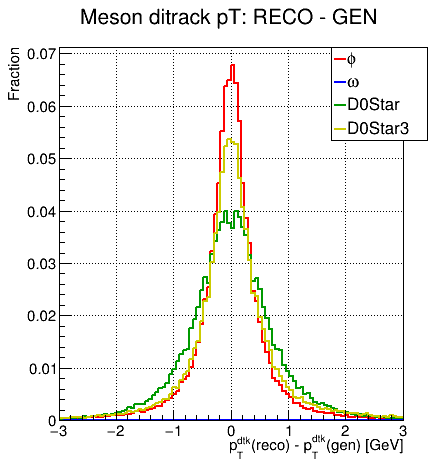
\includegraphics[width=0.45\mylength]{resources/plots/ditrack_residuals_pt.png}
                \caption{\footnotesize (a)}
        \end{subfigure}%
        \begin{subfigure}[t]{0.50\mylength}
                \centering
                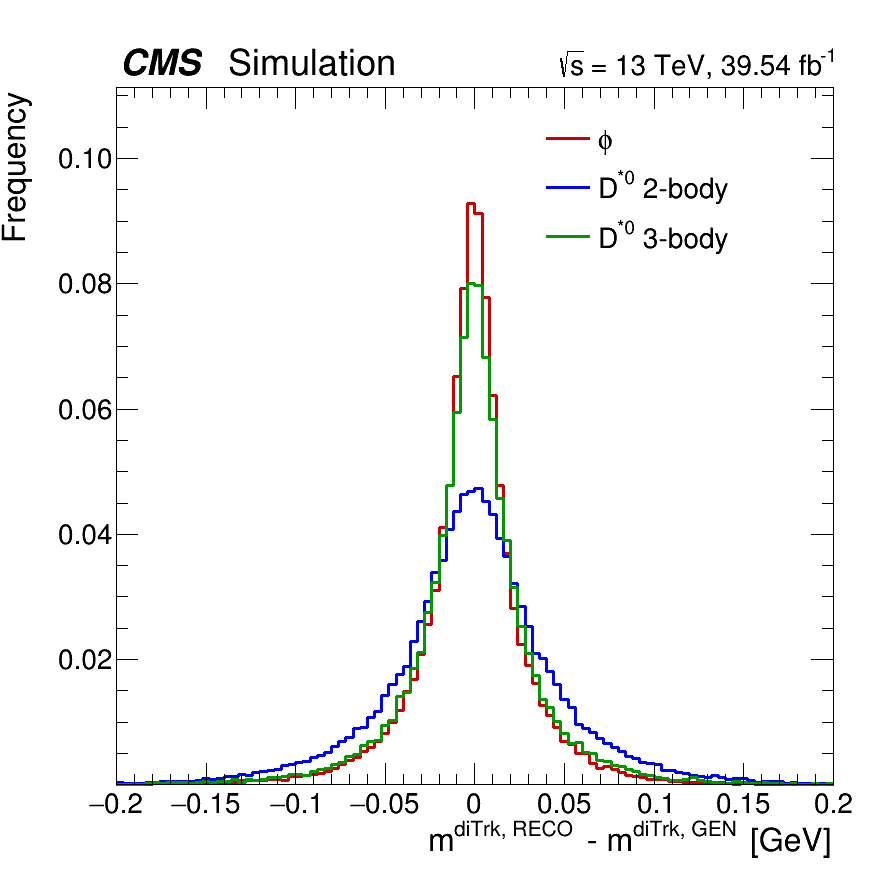
\includegraphics[width=0.45\mylength]{resources/plots/ditrack_residuals_mass.png}
                \caption{\footnotesize (b)}
        \end{subfigure}%\begin{subfigure}[t]{0.50\mylength}\baselineskip
        \vskip\baselineskip
        \vspace*{-0.1cm}
        \begin{subfigure}[t]{0.50\mylength}
                \centering
                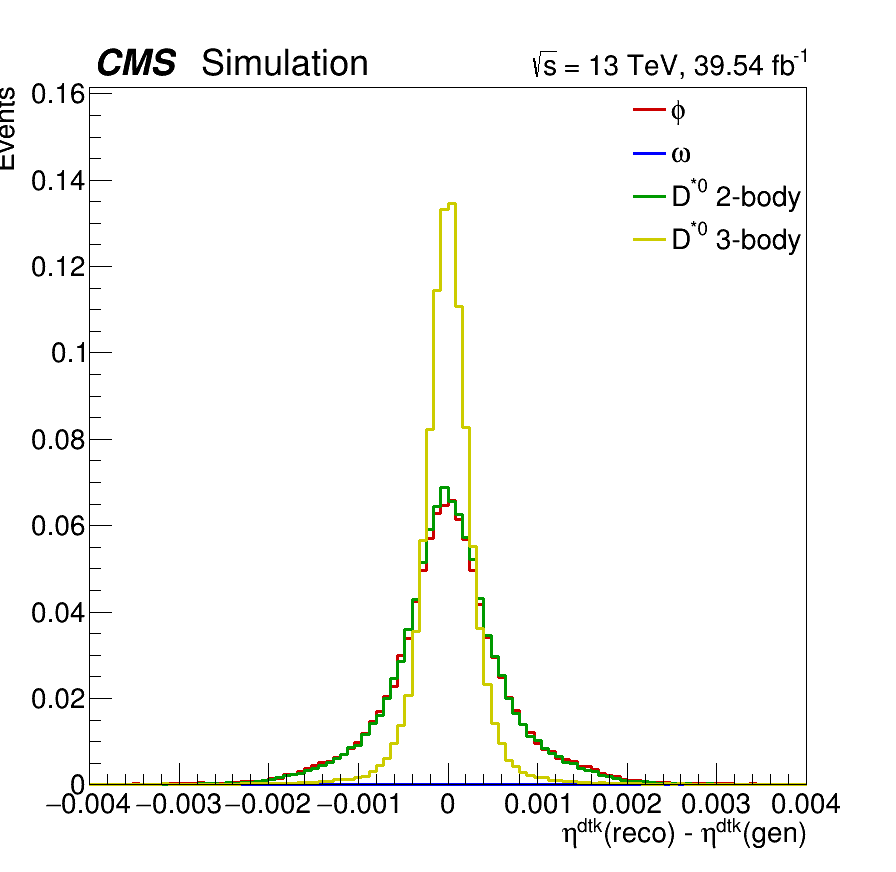
\includegraphics[width=0.45\mylength]{resources/plots/ditrack_residuals_eta.png}
                \caption{\footnotesize (c)}
        \end{subfigure}%\begin{subfigure}[t]{0.50\mylength}
        \begin{subfigure}[t]{0.50\mylength}
                \centering
                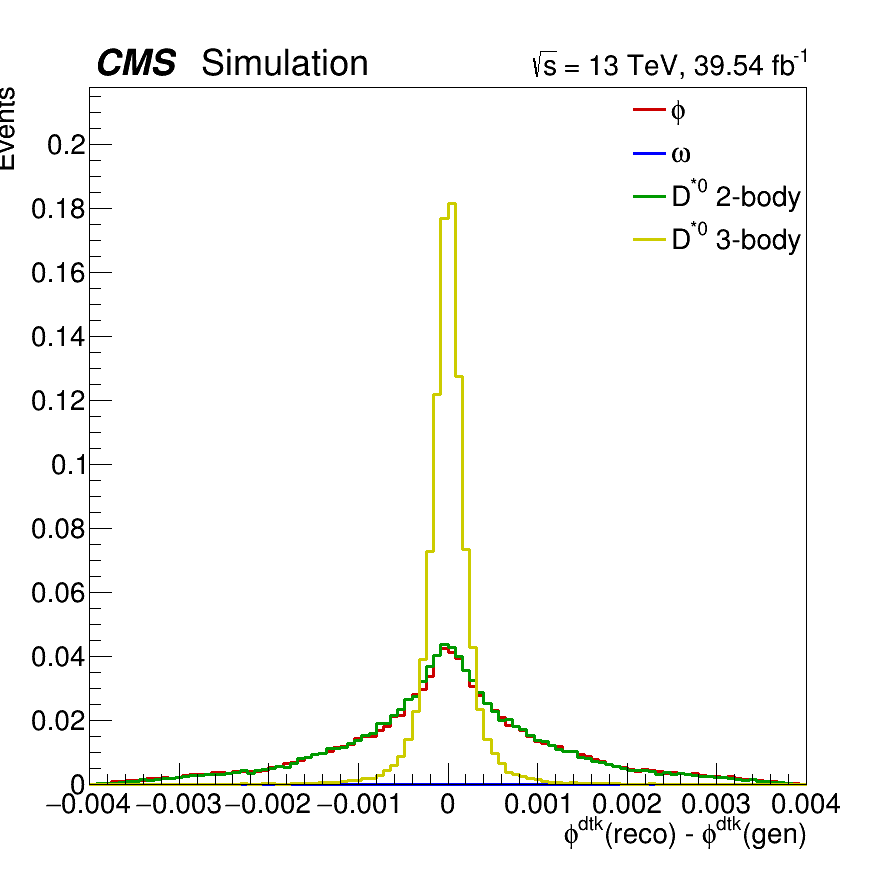
\includegraphics[width=0.45\mylength]{resources/plots/ditrack_residuals_phi.png}
                \caption{\footnotesize (d)}
        \end{subfigure}%
        \vspace*{-0.0cm}
        \caption{Ditrack residuals for the different four-momentum components of each decay channel. (a) is for $\pT$, (b) is for the mass, (c) is for $\eta$, and (d) is for $\phi$.}
        \label{fig:ditrack_residuals}
        \vspace*{-0.0cm}
    \end{figure}
    In each decay channel, the ditrack system variables are measured with remarkable accuracy. Figure \ref{fig:ditrack_residuals} displays the residuals of the ditrack transverse momentum, mass, $\eta$ and $\phi$ with respect to their generation-level MC value for every decay mode. All histograms are normalized to the same area for comparing the various channels. It is worth noting that, as the ditrack consists of a pair of charged tracks that can be precisely determined thanks to the silicon tracker, the direction -- $\eta$ and $\phi$ -- is accurately measured for all channels.

    The initial approach to reconstruct the full meson's transverse momentum is to sum the four-momenta of the ditrack system and those from the photons compatible with the decay of neutral particles. The main source of discrepancy between the full meson's transverse momenta and their generation-level MC values arises from the poorly reconstructed neutral particles. Given that the pions decay into softer photons that are hard to recover, many events exhibit missing energy, resulting in the full meson's $\pT$ being generally less energetic than expected. Figure \ref{fig:fullmeson_residuals_pt} shows the residuals of the full meson's transverse momentum with respect to their generation-level MC value for each decay mode.
    \begin{figure}[!ht]
        \captionsetup[subfigure]{labelformat=empty}
        \vspace*{-0.2cm}
        \centering
        \setlength{\mylength}{\textwidth}
        \includegraphics[width=0.75\mylength]{resources/plots/fullmeson_residuals_pt.png}
        \caption{Transverse momentum residuals for the full meson for each decay channel.}
        \label{fig:fullmeson_residuals_pt}
        \vspace*{-0.0cm}
    \end{figure}
    Both the $\phi$ and $\omega$ channels exhibit an asymmetric left shoulder, consistent with the hypothesis of missing energy from the neutral particle. The $D^{*0}$ 2-body, on the other hand, is more symmetric but displaced about 5 GeV, since the soft $\pi^{0}/\gamma$ from $D^{*0}\decaysto D^{0}\pi^{0}/\gamma$ typically carries around $\sim5$ GeV in energy. The right shoulder results from events in which we can recover one photon compatible with this missing neutral particle, which is only around $\sim 13\%$ of events. The $D^{*0}$ 3-body combines characteristics from all previous channels, and since it is missing two neutral particles it is noticeably shifted towards the lower end of the axis.

    To address this issue, dedicated Boosted Decision Trees (BDTs) have been implemented for each channel using the Toolkit for Multivariate Data Analysis for \verb+ROOT+ \cite{CERN:root}, also known as \verb+TMVA+ \cite{TMVA:2007ngy}. This machine learning (ML) technique will correct for the full meson's $\pT$. A boosted decision tree (BDT) is a ML binary classifier or regressor algorithm based on a flowchart-like structure in which each internal node represents a test on an attribute, each branch signifies the test's outcome, and each leaf node denotes a class level. For more detailed information, refer to Refs. \cite{TMVA:2007ngy, Coadou:2022nsh}.

    The variables used in all models are presented in Table \ref{tab:model_variables}.
    \begin{table}[!ht]
        \centering
        \begin{tabular}{|c|c|c|}
            \hline
            \multicolumn{3}{|c|}{\cellcolor{lightgray} Regression input variables} \\ \hline
            \cellcolor{lightgray}Dimensionless  &\cellcolor{lightgray}Dimensionful  &\cellcolor{lightgray}Normalised            \\\hline
            $\eta^{\text{diTrk}}$                           &$\pT^{\gamma_1}$       &$\pT^{\text{meson}}/\pT^{\gamma}$          \\
            $\Delta R^{\gamma_1, \text{diTrk}}$             &$\pT^{\gamma_2}$       &$\pT^{\text{meson}}/\pT^{\text{diTrk}}$    \\
            $\Delta R^{\gamma_2, \text{diTrk}}$             &$m^{\text{diTrk}}$     &           \\
            $\Delta R^{\text{diTrk}}$                       &$m^{\text{meson}}$ ($^*$)  &       \\
            $\Delta(\eta^{\gamma}, \eta^{\text{diTrk}})$    & & \\
            $\Delta(\phi^{\gamma}, \phi^{\text{diTrk}})$    & & \\
            \hline
        \end{tabular}
        \caption{Input variables for the BDTs. $\gamma_1$ and $\gamma_2$ represent photons from neutral particle decay, $\gamma$ stands for the Higgs boson decay photon. The asterisk denotes exclusion for $D^{*0}$ 2/3-body decay.}
        \label{tab:model_variables}
    \end{table}
    The variables labeled by $\gamma_1$ and $\gamma_2$ refer to the recovered photons compatible with the decay of the neutral particles, while $\gamma$ refers to the photon originating in the Higgs boson decay. The dimensionless variables $\Delta R^{\gamma_1, \text{diTrk}}$ and $\Delta R^{\gamma_2, \text{diTrk}}$ reference the angular separation between each photon and the ditrack system. $\Delta R^{\text{diTrk}}$ is the angular separation within the track pair. It is worth defining $\Delta(\eta^{\gamma}, \eta^{\text{diTrk}})$ and $\Delta(\phi^{\gamma}, \phi^{\text{diTrk}})$,
    \begin{equation*}
        \begin{aligned}
        \Delta(\eta^{\gamma}, \eta^{\text{diTrk}}) &= \eta^{\text{diTrk}} - \eta^{\gamma} \\
        \Delta(\phi^{\gamma}, \phi^{\text{diTrk}}) &= (\phi^{\text{diTrk}} - \phi^{\gamma}) \modu 2\pi \in[0, 2\pi)\ .
        \end{aligned}
    \end{equation*}
    The $\Delta(\phi^{\gamma}, \phi^{\text{diTrk}})$ definition has this form because the angular variable $\phi$ is periodic. The asterisk ($^*$) next to the full meson's mass indicates that this variable is not included for the $D^{*0}$ 2-body or 3-body decay, as in these channels, $m^{\text{meson}}$ is not very precisely determined.

    The variables in Table \ref{tab:model_variables} have been thoughtfully selected after many model iterations, ensuring low correlation between them and with the Higgs boson invariant mass, while maintaining reasonable predictive power.

    All the models have been trained to predict not the correct value of the full meson's transverse momentum, but a scale factor $\pT^{\text{meson, GEN}}/\pT^{\text{meson, RECO}}$ instead. This scale factor represents the adjustment needed for the reconstructed $\pT$ to match its generation-level MC value. The motivation for this approach is to avoid biasing the model by predicting a dimensionless variable.

    We implemented the BDTs using the \verb+TMVA+ framework, specifically the
\begin{small}
\vspace*{-6pt}
\begin{verbatim}
TMVA::Factory.BookMethod(dataloader, TMVA::Types::kBDT, "modelName", "<options>");
\end{verbatim}
\vspace*{-6pt}
\end{small}
    method, with the ML regressor \verb+TMVA::Types::kBDT+. To prevent overtraining, we employed cross-validation by rotating the training and testing samples. Specifically, the signal MC was divided into three subsets: A, B, and C. Three models with identical hyperparameters were trained on A+B (B+C / C+A) and tested on C (A / B). This approach ensures all the available data is used to train the models while testing them on signal MC that was not used for training. To recover all the signal events, these three models were then applied to their respective testing subsets. Afterward, all the subsets were combined once more, resulting in a complete set of events.

    \begin{figure}[!ht]
        \captionsetup[subfigure]{labelformat=empty}
        \vspace*{-0.2cm}
        \centering
        \setlength{\mylength}{\textwidth}
        \begin{subfigure}[t]{0.50\mylength}
            \centering
            \includegraphics[width=0.45\mylength]{resources/plots/Phi3_model_pt.png}
            \caption{\footnotesize (a)}
        \end{subfigure}%
        \begin{subfigure}[t]{0.50\mylength}
            \centering
            \includegraphics[width=0.45\mylength]{resources/plots/Phi3_model_pt_residuals.png}
            \caption{\footnotesize (b)}
        \end{subfigure}%\begin{subfigure}[t]{0.50\mylength}\baselineskip
        \vskip\baselineskip
        \vspace*{-0.1cm}
        \begin{subfigure}[t]{0.50\mylength}
            \centering
            \includegraphics[width=0.45\mylength]{resources/plots/Omega_model_pt.png}
            \caption{\footnotesize (c)}
        \end{subfigure}%
        \begin{subfigure}[t]{0.50\mylength}
            \centering
            \includegraphics[width=0.45\mylength]{resources/plots/Omega_model_pt_residuals.png}
            \caption{\footnotesize (d)}
        \end{subfigure}%\begin{subfigure}[t]{0.50\mylength}\baselineskip
    \caption{Transverse momentum of the $\phi$ and $\omega$ mesons. (a/c) Display the generation-level MC transverse momenta in blue, the prediction by the BDT in red, and the recovery by the initial approach in green, for the $\phi/\omega$ mesons, respectively. (b/d) Show the residuals with (red) and without (green) the BDT prediction, for the $\phi/\omega$ mesons, respectively.}
    \label{fig:pt_residuals_model_omega_phi}
        \vspace*{-0.0cm}
    \end{figure}
    The hyperparameters for each model are available in Table \ref{tab:hyperparameters_models} in Appendix \ref{sec:appendix_models}. Figures \ref{fig:pt_residuals_model_omega_phi} and \ref{fig:pt_residuals_model_d0star} compare the generation-level MC transverse momentum with the reconstruction values, both with and without regression, and show the residuals for each channel.
    \begin{figure}[!ht]
        \captionsetup[subfigure]{labelformat=empty}
        \vspace*{-0.2cm}
        \centering
        \setlength{\mylength}{\textwidth}
        \begin{subfigure}[t]{0.50\mylength}
            \centering
            \includegraphics[width=0.45\mylength]{resources/plots/D0Star_2body_model_pt.png}
            \caption{\footnotesize (a)}
        \end{subfigure}%
        \begin{subfigure}[t]{0.50\mylength}
            \centering
            \includegraphics[width=0.45\mylength]{resources/plots/D0Star_2body_model_pt_residuals.png}
            \caption{\footnotesize (b)}
        \end{subfigure}%\begin{subfigure}[t]{0.50\mylength}\baselineskip
        \vskip\baselineskip
        \vspace*{-0.1cm}
        \begin{subfigure}[t]{0.50\mylength}
            \centering
            \includegraphics[width=0.45\mylength]{resources/plots/D0Star_3body_model_pt.png}
            \caption{\footnotesize (c)}
        \end{subfigure}%
        \begin{subfigure}[t]{0.50\mylength}
            \centering
            \includegraphics[width=0.45\mylength]{resources/plots/D0Star_3body_model_pt_residuals.png}
            \caption{\footnotesize (d)}
        \end{subfigure}%\begin{subfigure}[t]{0.50\mylength}\baselineskip
    \caption{Transverse momentum of the $D^{*0}$ meson in both the 2-body and 3-body decay channels. (a/c) Display the generation-level MC transverse momenta in blue, the prediction by the BDT in red, and the recovery by the initial approach in green, for the 2/3-body decay channel, respectively. (b/d) Show the residuals with (red) and without (green) the BDT prediction, for the 2/3-body decay channel, respectively.}
    \label{fig:pt_residuals_model_d0star}
        \vspace*{-0.0cm}
    \end{figure}

    Both channels displayed in Figure \ref{fig:pt_residuals_model_omega_phi} are quite similar. For both full mesons, the predicted transverse momentum spectrum aligns well with the generation-level one. Additionally, the residuals for the predicted values are centered around the origin and symmetric, indicating that the predicted $\pT$ no longer exhibits missing energy. The 2-body decay channel presented in Figure \ref{fig:pt_residuals_model_d0star} shows that the model accurately shifts by around 5 GeV, as the residuals are narrow around 0 GeV instead of around -5 GeV, and it is also more symmetric than the initially reconstructed $\pT$. \todo{The 3-body decay channel shown in Figure \ref{fig:pt_residuals_model_d0star} bla bla bla}.

    Table \ref{tab:models_pt_RMSE} shows the root mean squared errors with respect to generation-level transverse momentum, both with and without the BDT regression, for each channel. Applying the transverse momenta regression noticeably improves the value and reduces the error for all channels by around 35\%.
    \begin{table}[!ht]
        \centering
        \begin{tabular}{|l|c|C{3.1cm}@{}c|}
            \hline
            \cellcolor{lightgray}Decay channel & \cellcolor{lightgray}RMSE without $\pT$ regression & \multicolumn{2}{c|}{\cellcolor{lightgray}RMSE with $\pT$ regression} \\ \hline
            $\phi$          &5.124 GeV   &3.480 GeV  & (-32\%)  \\
            $\omega$        &5.058 GeV   &3.339 GeV  & (-34\%)  \\
            $D^{*0}$ 2-body &3.132 GeV   &1.871 GeV  & (-40\%)  \\
            \r$D^{*0}$ 3-body &\r xx.x GeV   &x\r x.x GeV  & \r(-xx\%)  \\
            \hline
            \end{tabular}
        \caption{Root mean squared errors of the full meson's transverse momentum with and without the BDT regression for each decay mode.}
        \label{tab:models_pt_RMSE}
    \end{table}
    The applied BDTs not only significantly reduce the error in the transverse momentum of the full meson for every channel but also restore the symmetric residual shape of the variable. This indicates that the estimated $pT$ values are as likely to be underestimated as to be overestimated, accounting for the missing energy from the undetected neutral particles. This reduction in the width of the residuals will directly lead to an improved, lower upper limit on the Higgs boson branching fraction.

    A crucial consideration in developing any ML model is overtraining, and this case is no exception. This is the primary reason a dimensionless scale factor was predicted rather than the direct value of the momentum. In our situation, overtraining can be directly detected by examining the background shape after applying the regression. If the model learns that, regardless of the input, the predicted value should lead to a peak around 125 GeV when constructing the Higgs invariant mass variable, we know it is overtrained and biased and needs to be rejected. To address this and reject biased models, we introduced a \textit{background shaping function (BSF)} that provides a dimensionless metric which increases as the model becomes more biased. The BSF we developed for measuring each model is defined to be
    \begin{equation*}
        BSF \propto -A\log{(\mu-125)^2} + B N + C \sqrt{b}\ ,
    \end{equation*}
    where $A$, $B$, and $C$ are constants, $\mu$ is the peak of a fitted double-sided Crystal Ball\footnote{A double-sided Crystal Ball function, named after the Crystal Ball Collaboration \cite{A2:CB}, is a probability density function (PDF) commonly used in high-energy physics (HEP). It is built from a Gaussian center and two asymmetric tails modeled by power-law functions. Additional details about this PDF and its implementation in ROOT can be found in Ref. \cite{CERN:root_CB}.} (CB) to the Higgs boson's invariant mass constructed from background MC events, $N$ is the normalization constant of the Crystal Ball, and $b$ is the number of events in the interval $(117, 133)$ GeV of the Higgs boson's invariant mass. Note that the BSF depends only on background events, especially in reconstructing the Higgs boson's invariant mass. The first factor penalizes the model more when the background Higgs boson's invariant mass shape peaks around $m_H=125\ \GeV$, because the background should be flat or asymptotically falling near that value. The remaining two factors account for the number of events near the expected signal peak. More background events result in a smaller and thus worse signal-to-background ratio, a quantity we want to maximize to improve the computation of upper limits.

    Figure \ref{fig:BSF_vs_RMSE_phi} shows the BSF as a function of the RMSE of different models applied to reconstruct the transverse momentum of the $\phi$ meson.
    \begin{figure}[!ht]
        \captionsetup[subfigure]{labelformat=empty}
        \vspace*{-0.2cm}
        \centering
        \setlength{\mylength}{\textwidth}
        \includegraphics[width=0.85\mylength]{resources/plots/BSF_vs_RMSE_phi.png}
        \caption{Background shaping function (BSF) as a function of the root mean squared error (RMSE) of the $\pT$ for various models of the $\phi$ decay channel. The reconstructed and used model's values are shown in teal and yellow, respectively.}
        \label{fig:BSF_vs_RMSE_phi}
        \vspace*{-0.0cm}
    \end{figure}
    The studied models follow an expected trend: as the BSF increases, and consequently, the model becomes more biased, the RMSE decreases. All decay channela have a similar behaviour, so only the $\phi$ channel is shown. To select one model from the many tens of thousands we tested, compromises must be made since there is a trade-off between not shaping the background and significantly improving the error. We identified different BSF thresholds for each decay channel, considering that each decay involves a different number of events, directly related to the BSF. Thus, it is not meaningful to compare BSF values across channels; it is only relevant to compare them within a single channel. For the $\phi$ decay channel, we find a value of around 12 by directly examining the shape of the background Higgs boson's invariant mass.

\end{myitemlist}

After having presented all the techniques used to recover the meson, we are able to perform some selection cuts to maintain as much signal events as possible, while rejecting as many background events. Tables \ref{tab:meson_selection_1} and \ref{tab:meson_selection_2} summarize the meson candidate selection criteria used for each decay channel, where $\gamma^{\text{diTrk}}$ are the photons from neutral particle decays, and $\gamma_\text{H}$ refers to the photon originating in the Higgs boson decay.
\begin{table}[!ht]
    \centering
    \begin{tabular}{|l|c|c|}
        \hline
        \cellcolor{lightgray}Variable & \cellcolor{lightgray}$\phi(\pi^{\pm}\pi^{\mp}\pi^{0})$ & \cellcolor{lightgray}$\omega(\pi^{\pm}\pi^{\mp}\pi^{0})$ \\ \hline
        Meson mass                                              &$0.96\pm0.26$ GeV  &$0.785\pm0.215$ GeV    \\
        Ditrack mass                                            &$0.59\pm0.25$ GeV  &$0.47\pm0.15$ GeV      \\
        $\pT^{\text{diTrk}}$                                    &$>10$ GeV          &$>15$ GeV              \\
        $\pT^{\text{leadTrk}}$                                  &$>5$ GeV           &$>8$ GeV               \\
        $\#\gamma^{\text{diTrk}}$                               &$>0$               &$>0$                   \\
        $\Delta(\phi^{\text{diTrk}}, \phi^{\gamma_\text{H}})$   &$\pi\pm2.3$    &$\pi\pm2.3$        \\
        $\Delta(\eta^{\text{diTrk}}, \eta^{\gamma_\text{H}})$   &$0\pm1.9$          &$0\pm1.9$              \\
        Iso                                                     &$>0.95$            &$>0.95$                \\
        \hline
        \end{tabular}
    \caption{Selection criteria applied to the $\phi$ and $\omega$ mesons used in the analysis.}
    \label{tab:meson_selection_1}
\end{table}

\begin{table}[!ht]
    \centering
    \begin{tabular}{|l|c|c|}
        \hline
        \cellcolor{lightgray}Variable & \cellcolor{lightgray}$D^{*0}(K^{\mp}\pi^{\pm}{\scriptstyle(\pi^{0}/\gamma)})$ & \cellcolor{lightgray}$D^{*0}(K^{\mp}\pi^{\pm}\pi^{0}{\scriptstyle(\pi^{0}/\gamma)})$ \\ \hline
        Meson mass                                              &                   &$1.55\pm 0.65$ GeV  \\
        Ditrack mass                                            &$1.865\pm0.060$ GeV&$1.18\pm 0.57$ GeV  \\
        $\pT^{\text{diTrk}}$                                    &$>40$ GeV          &$>20$ GeV           \\
        $\pT^{\text{leadTrk}}$                                  &$>21$ GeV          &$>10$ GeV           \\
        $\pT^{\text{subLeadTrk}}$                               &$>5$ GeV           &$>3$ GeV           \\
        $\#\gamma^{\text{diTrk}}$                               &                   &$>0$               \\
        $\Delta(\phi^{\text{diTrk}}, \phi^{\gamma_\text{H}})$   &$\pi\pm2.3$        &$\pi\pm2.3$        \\
        $\Delta(\eta^{\text{diTrk}}, \eta^{\gamma_\text{H}})$   &$0\pm1.9$          &$0\pm1.9$           \\
        Iso                                                     &$>0.91$            &$>0.95$             \\
        \hline
        \end{tabular}
    \caption{Selection criteria applied to each channel of the $D^{*0}$ meson decay used in the analysis.}
    \label{tab:meson_selection_2}
\end{table}

In most of the events the full meson and the photon are back-to-back, so $\Delta(\phi^{\text{diTrk}}, \phi^{\gamma_\text{H}})$ is centered around $\pi$. We select highly isolated particles as this significantly reduces background contribution.

%\section{Corrections to data and simulations}\label{sec:corrections}

%\todo{Pileup reweighting, L1 prefiring corrections, photon scale and resolution, photon mvaid efficiency, Lepton ID reconstruction efficiency and energy scale (?), meson reconstruction, triggers scale factors}
%\newpage
\section{Event selection}\label{sec:event_selection}

The analysis described here searches for the Higgs boson decaying to a photon and to either a $\phi$, $\omega$ or $D^{*0}$ meson. The signal features narrow peaks in the ditrack, the full meson (M), and M + $\gamma$ distributions over the SM backgrounds. These resonances can be fully reconstructed thanks to the excellent resolution of the CMS detector in measuring of the photon energy and track momentum. Nevertheless, the accuracy of these three-body decays is not as good as in other exotic Higgs boson decays of the same type, but where the vector meson decays only into a pair of charged tracks, currently under analysis by the PPC at MIT. The presence of a third, neutral particle makes reconstructing of the full meson more intricate and reduces the precision of the recovered four-momentum.

The $\phi\gamma$, $\omega\gamma$ and $D^{*0}\gamma$ exclusive final states are very similar. Meson candidates are paired with photon candidates to form M$\gamma$ candidates. When multiple photon candidates meeting the selection criteria outlined in Section \ref{sec:objects} are present, the one with the highest transverse momentum is chosen. Similarly, when multiple meson candidates satisfying the selection criteria described in Section \ref{sec:meson_reconstruction} are found, the one with a mass closest to the theoretical mass value of the meson is chosen.

The $\phi\gamma$ and $\omega\gamma$ channels in particular closely resemble each other, both decaying into $\pi^{+}\pi^{-}\pi^0$ and having similar masses and decay widths. The $D^{*0}$ 2-body decay can effectively be treated as a three-body decay, $D^{*0}\decaysto K^{\mp}\pi^{\pm}\pi^0/\gamma$, due to its short lifetime. The main difference between this channel and the $\phi/\omega$ channel is that in the $\phi/\omega$ case, the three pions carry, on average, approximately the same energy, while for $D^{*0}$ the neutral particle is very soft, carrying only around 5 GeV. Finally, the $D^{*0}$ 3-body decay can effectively be treated as a 4-body decay for the same reason, with 2 charged tracks, one soft neutral particle, and one neutral pion. This last case shares similarities with the previous ones.

This thesis exclusively targets Higgs boson production via gluon fusion (ggH). To focus on this production mode, events with additional charged leptons with $\pT$ > 10 GeV are vetoed. Events with two or more jets having $\pT$ > 30 GeV and $\abs{\eta} < 4.7$, exhibiting a significant pseudorapidity gap ($\abs{\Delta\eta_{jj}} > 3$), and with an invariant mass $m_{jj} > 300\ \GeV$, are excluded from this category. Jets should not overlap with the meson and photon forming the Higgs boson candidate and must meet the criteria mentioned in Section \ref{sec:objects}. Table \ref{tab:triggers} summarizes the selection criteria for this production mode, which must additionally satisfy the selection rules of the tau-like trigger described in Section \ref{subsec:data_tau_trigger}.

\begin{table}[!ht]
    \centering
    \begin{tabular}{|c|c|c|c|}
    \hline
    \cellcolor{lightgray}Target signal   & \cellcolor{lightgray}Trigger & \cellcolor{lightgray}Selection & \cellcolor{lightgray}Integrated luminosity (fb$^{-1}$)\\ \hline
    \multirow{3}{*}{ggH}&\multirow{3}{*}{tau-like}  &no e/$\mu$ with $\pT$ > 10 GeV & \multirow{3}{*}{39.54 (2018)}\\
                        &                           &no dijet pair with $\abs{\Delta\eta_{jj}} > 3$ & \\
                        &                           &and $m_{jj} > 300\ \GeV$                       & \\
    \hline
    \end{tabular}
    \caption{Selection criteria used for the ggH production mode, alongside the integrated luminosity provided by CMS compatible with these criteria.}
    \label{tab:triggers}
\end{table}
The product of signal selection efficiency and acceptance ($\epsilon$A) corresponds to the fraction of MC simulated signal events that pass the selection.
\begin{table}[!ht]
    \centering
    \begin{tabular}{|c|c|c|c|c|}
        \hline
        \cellcolor{lightgray}Selection &\cellcolor{lightgray}$\text{H}\decaysto \phi\gamma$ &\cellcolor{lightgray}$\text{H}\decaysto \omega\gamma$ &\cellcolor{lightgray}$\text{H}\decaysto D^{*0}\gamma$ {\scriptsize(2-body)}&\cellcolor{lightgray}$\text{H}\decaysto D^{*0}\gamma$ {\scriptsize(3-body)}\\ \hline
        trigger                                     & 24\%  & 23\%  & 17\%  & 19\% \\
        1 good $\gamma$                             & 89\%  & 90\%  & 89\%  & 90\% \\
        1 good meson                                & 42\%  & 40\%  & 64\%  & 32\% \\
        0, 1 jet, 2 with $\abs{\Delta\eta_{jj}}$    & 94\%  & 94\%  & 94\%  & 93\% \\
        0 leptons                                   & 99\%  & 98\%  & 99\%  & 99\% \\ \hline
        Cumulative $\epsilon$A                      & 8.2\%  & 7.9\%  & 9.0\%  & 5.1\% \\
        \hline
        \end{tabular}
    \caption{Signal selection efficiency for all decay channels.}
    \label{tab:selection_efficiency}
\end{table}
Table \ref{tab:selection_efficiency} reports the signal cut flow. The efficiencies for the $\phi$ and $\omega$ channels are consistently similar throughout the selection flow. It can be observed that the tau trigger is less efficient for the $D^{*0}$ decay mode compared to the other channels, resulting in a lower cumulative acceptance.

These strict cuts (selecting approximately only one in eleven signal events) will eliminate most of the background events, which for the ggH enriched channel, it dominantly consists of $\gamma$ + multijet process, with a smaller contribution arising from QCD multijet. The 2-body $D^{*0}$ decay is expected to have less background compared to the $\phi$, $\omega$ and 3-body $D^{*0}$ decays, as in the 2-body case the ditrack is a real resonance with a narrow width. Additionally, the $\omega$ channel is expected to have also less background than the $\phi$ and 3-body $D^{*0}$ decays due to its sharper decay width.

\begin{figure}[!ht]
    \captionsetup[subfigure]{labelformat=empty}
    \vspace*{-0.2cm}
    \centering
    \setlength{\mylength}{\textwidth}
    \begin{subfigure}[t]{0.50\mylength}
        \centering
        \includegraphics[width=0.45\mylength]{resources/plots/Phi3_dtrk_mass.png}
        \caption{\footnotesize (a)}
    \end{subfigure}%
    \begin{subfigure}[t]{0.50\mylength}
        \centering
        \includegraphics[width=0.45\mylength]{resources/plots/Omega_dtrk_mass.png}
        \caption{\footnotesize (b)}
    \end{subfigure}%\begin{subfigure}[t]{0.50\mylength}\baselineskip
    \vskip\baselineskip
    \vspace*{-0.1cm}
    \begin{subfigure}[t]{0.50\mylength}
        \centering
        \includegraphics[width=0.45\mylength]{resources/plots/D0Star_2body_dtrk_mass.png}
        \caption{\footnotesize (c)}
    \end{subfigure}%
    \begin{subfigure}[t]{0.50\mylength}
        \centering
        \includegraphics[width=0.45\mylength]{resources/plots/D0Star_3body_dtrk_mass.png}
        \caption{\footnotesize (d)}
    \end{subfigure}%\begin{subfigure}[t]{0.50\mylength}\baselineskip
\caption{Ditrack mass of the different studied decay modes. (a) $\phi$ channel, (b) $\omega$ channel, (c) $D^{*0}$ 2-body channel, and (d) $D^{*0}$ 3-body channel. The MC background is shown in orange, scatter points represent real data, and the signal, in red, is normalized to the data for better visualization.}
\label{fig:ditrack_mass_data}
    \vspace*{-0.0cm}
\end{figure}

Figure \ref{fig:ditrack_mass_data} displays the invariant mass of the ditrack system. In all decay channels (and in subsequent figures showing other kinematic variables), the MC background underestimates the data as it only considers the dominant contribution at LO. The data is a factor of around 20\% larger, but the estimated limits are ultimately calculated using the data for the background fit. The MC background serves the purpose of helping us comprehend the behavior of the involved processes.

In Figure \ref{fig:ditrack_mass_data} (c), a sharper resonance is observed because, as mentioned earlier, the ditrack system is a real $D^{0}$ meson. In contrast, for the other cases (where the ditrack is not a real particle), the invariant ditrack mass is considerably wider. Across all decay modes, the MC background is consistent with the data.

\begin{figure}[!ht]
    \captionsetup[subfigure]{labelformat=empty}
    \vspace*{-0.2cm}
    \centering
    \setlength{\mylength}{\textwidth}
    \begin{subfigure}[t]{0.50\mylength}
        \centering
        \includegraphics[width=0.45\mylength]{resources/plots/Phi3_mass.png}
        \caption{\footnotesize (a)}
    \end{subfigure}%
    \begin{subfigure}[t]{0.50\mylength}
        \centering
        \includegraphics[width=0.45\mylength]{resources/plots/Omega_mass.png}
        \caption{\footnotesize (b)}
    \end{subfigure}%\begin{subfigure}[t]{0.50\mylength}\baselineskip
    \vskip\baselineskip
    \vspace*{-0.1cm}
    \begin{subfigure}[t]{0.50\mylength}
        \centering
        \includegraphics[width=0.45\mylength]{resources/plots/D0Star_2body_mass.png}
        \caption{\footnotesize (c)}
    \end{subfigure}%
    \begin{subfigure}[t]{0.50\mylength}
        \centering
        \includegraphics[width=0.45\mylength]{resources/plots/D0Star_3body_mass.png}
        \caption{\footnotesize (d)}
    \end{subfigure}%\begin{subfigure}[t]{0.50\mylength}\baselineskip
\caption{Full meson's mass of the different studied decay modes. (a) $\phi$ channel, (b) $\omega$ channel, (c) $D^{*0}$ 2-body channel, and (d) $D^{*0}$ 3-body channel. The MC background is shown in orange, scatter points represent real data, and the signal, in red, is normalized to the data for better visualization.}
\label{fig:full_mass_data}
    \vspace*{-0.0cm}
\end{figure}

Figure \ref{fig:full_mass_data} displays the mass of the full meson. This variable is sharper than the ditrack system's mass in all channels because it consists of a real meson. However, for the $D^{*0}$ 2-body decay mode, it is not well reconstructed. In approximately $\sim 87\%$ of events, no photon compatible with the decay of a neutral particle is recovered, and therefore the computed full mass is the same as the ditrack system's mass. This is why this variable is not used in the BDT for regressing the transverse momentum (see Section \ref{sec:meson_reconstruction}). All decay modes exhibit missing energy, as all channels have an asymmetric left shoulder.

\begin{figure}[!ht]
    \captionsetup[subfigure]{labelformat=empty}
    \vspace*{-0.2cm}
    \centering
    \setlength{\mylength}{\textwidth}
    \begin{subfigure}[t]{0.50\mylength}
        \centering
        \includegraphics[width=0.45\mylength]{resources/plots/Phi3_photon_pt.png}
        \caption{\footnotesize (a)}
    \end{subfigure}%
    \begin{subfigure}[t]{0.50\mylength}
        \centering
        \includegraphics[width=0.45\mylength]{resources/plots/Omega_photon_pt.png}
        \caption{\footnotesize (b)}
    \end{subfigure}%\begin{subfigure}[t]{0.50\mylength}\baselineskip
    \vskip\baselineskip
    \vspace*{-0.1cm}
    \begin{subfigure}[t]{0.50\mylength}
        \centering
        \includegraphics[width=0.45\mylength]{resources/plots/D0Star_2body_photon_pt.png}
        \caption{\footnotesize (c)}
    \end{subfigure}%
    \begin{subfigure}[t]{0.50\mylength}
        \centering
        \includegraphics[width=0.45\mylength]{resources/plots/D0Star_3body_photon_pt.png}
        \caption{\footnotesize (d)}
    \end{subfigure}%\begin{subfigure}[t]{0.50\mylength}\baselineskip
\caption{Transverse momentum $\pT$ of the primary photon from the Higgs boson decay, for the different studied decay modes. (a) $\phi$ channel, (b) $\omega$ channel, (c) $D^{*0}$ 2-body channel, and (d) $D^{*0}$ 3-body channel. The MC background is shown in orange, scatter points represent real data, and the signal, in red, is normalized to the data for better visualization.}
\label{fig:photon_pt_data}
    \vspace*{-0.0cm}
\end{figure}

Figure \ref{fig:photon_pt_data} presents the transverse momentum of the primary photon originating directly from the Higgs boson decay. The signal peaks at around 60 GeV for all channels, which is roughly half of the Higgs boson's mass. This is consistent with Figure \ref{fig:full_pt_data}, which shows the transverse momentum of each meson. In every channel, the signal also peaks around 60 GeV, which with the transverse momentum of the photon adds up to the 125 GeV of the Higgs boson's mass.

\begin{figure}[!ht]
    \captionsetup[subfigure]{labelformat=empty}
    \vspace*{-0.2cm}
    \centering
    \setlength{\mylength}{\textwidth}
    \begin{subfigure}[t]{0.50\mylength}
        \centering
        \includegraphics[width=0.45\mylength]{resources/plots/Phi3_pt.png}
        \caption{\footnotesize (a)}
    \end{subfigure}%
    \begin{subfigure}[t]{0.50\mylength}
        \centering
        \includegraphics[width=0.45\mylength]{resources/plots/Omega_pt.png}
        \caption{\footnotesize (b)}
    \end{subfigure}%\begin{subfigure}[t]{0.50\mylength}\baselineskip
    \vskip\baselineskip
    \vspace*{-0.1cm}
    \begin{subfigure}[t]{0.50\mylength}
        \centering
        \includegraphics[width=0.45\mylength]{resources/plots/D0Star_2body_pt.png}
        \caption{\footnotesize (c)}
    \end{subfigure}%
    \begin{subfigure}[t]{0.50\mylength}
        \centering
        \includegraphics[width=0.45\mylength]{resources/plots/D0Star_3body_pt.png}
        \caption{\footnotesize (d)}
    \end{subfigure}%\begin{subfigure}[t]{0.50\mylength}\baselineskip
\caption{Transverse momentum $\pT$ of the full meson for the different studied decay modes. (a) $\phi$ channel, (b) $\omega$ channel, (c) $D^{*0}$ 2-body channel, and (d) $D^{*0}$ 3-body channel. The MC background is shown in orange, scatter points represent real data, and the signal, in red, is normalized to the data for better visualization.}
\label{fig:full_pt_data}
    \vspace*{-0.0cm}
\end{figure}

\begin{figure}[!ht]
    \captionsetup[subfigure]{labelformat=empty}
    \vspace*{-0.2cm}
    \centering
    \setlength{\mylength}{\textwidth}
    \begin{subfigure}[t]{0.50\mylength}
        \centering
        \includegraphics[width=0.45\mylength]{resources/plots/Phi3_lead_pt.png}
        \caption{\footnotesize (a)}
    \end{subfigure}%
    \begin{subfigure}[t]{0.50\mylength}
        \centering
        \includegraphics[width=0.45\mylength]{resources/plots/Omega_lead_pt.png}
        \caption{\footnotesize (b)}
    \end{subfigure}%\begin{subfigure}[t]{0.50\mylength}\baselineskip
    \vskip\baselineskip
    \vspace*{-0.1cm}
    \begin{subfigure}[t]{0.50\mylength}
        \centering
        \includegraphics[width=0.45\mylength]{resources/plots/D0Star_2body_lead_pt.png}
        \caption{\footnotesize (c)}
    \end{subfigure}%
    \begin{subfigure}[t]{0.50\mylength}
        \centering
        \includegraphics[width=0.45\mylength]{resources/plots/D0Star_3body_lead_pt.png}
        \caption{\footnotesize (d)}
    \end{subfigure}%\begin{subfigure}[t]{0.50\mylength}\baselineskip
\caption{Transverse momentum $\pT$ of the leading charged track for the different studied decay modes. (a) $\phi$ channel, (b) $\omega$ channel, (c) $D^{*0}$ 2-body channel, and (d) $D^{*0}$ 3-body channel. The MC background is shown in orange, scatter points represent real data, and the signal, in red, is normalized to the data for better visualization.}
\label{fig:lead_pt_data}
    \vspace*{-0.0cm}
\end{figure}

\newpage

Figures \ref{fig:lead_pt_data} and \ref{fig:sublead_pt_data} illustrate the transverse momentum of the charged leading and subleading tracks for each decay mode. All channels show a similar shape for the signal. However, it is worth noting that in the $D^{*0}$ 2-body decay, both the leading and subleading tracks are more energetic, as this is the only scenario where $D^{0}$ decays into only two charged tracks (the neutral particle from $D^{*0}\decaysto D^{0}\pi^{0}/\gamma$ typically carries around $\sim5$ GeV in energy).

\begin{figure}[!ht]
    \captionsetup[subfigure]{labelformat=empty}
    \vspace*{-0.2cm}
    \centering
    \setlength{\mylength}{\textwidth}
    \begin{subfigure}[t]{0.50\mylength}
        \centering
        \includegraphics[width=0.45\mylength]{resources/plots/Phi3_sublead_pt.png}
        \caption{\footnotesize (a)}
    \end{subfigure}%
    \begin{subfigure}[t]{0.50\mylength}
        \centering
        \includegraphics[width=0.45\mylength]{resources/plots/Omega_sublead_pt.png}
        \caption{\footnotesize (b)}
    \end{subfigure}%\begin{subfigure}[t]{0.50\mylength}\baselineskip
    \vskip\baselineskip
    \vspace*{-0.1cm}
    \begin{subfigure}[t]{0.50\mylength}
        \centering
        \includegraphics[width=0.45\mylength]{resources/plots/D0Star_2body_sublead_pt.png}
        \caption{\footnotesize (c)}
    \end{subfigure}%
    \begin{subfigure}[t]{0.50\mylength}
        \centering
        \includegraphics[width=0.45\mylength]{resources/plots/D0Star_3body_sublead_pt.png}
        \caption{\footnotesize (d)}
    \end{subfigure}%\begin{subfigure}[t]{0.50\mylength}\baselineskip
\caption{Transverse momentum $\pT$ of the subleading charged track for the different studied decay modes. (a) $\phi$ channel, (b) $\omega$ channel, (c) $D^{*0}$ 2-body channel, and (d) $D^{*0}$ 3-body channel. The MC background is shown in orange, scatter points represent real data, and the signal, in red, is normalized to the data for better visualization.}
\label{fig:sublead_pt_data}
    \vspace*{-0.0cm}
\end{figure}

\section{Signal and background modelling \todo{ADD 2D FIT}}\label{sec:modelling}

The potential Higgs boson signal is obtained by fitting the invariant mass distribution $M_{\gamma, M}$ for each decay mode separately, since the signal is expected to show a peak over a monotonous background. Both the signal and background are directly estimated from MC (signal) or data (background) by fitting the photon-meson mass spectrum with analytical functions. The RooFit framework \cite{CERN:root_roofit}, a toolkit provided within the ROOT module for modeling the expected event distribution, is used for this purpose, and a binned maximum likelihood fit is conducted.
\begin{figure}[!ht]
    \captionsetup[subfigure]{labelformat=empty}
    \vspace*{-0.2cm}
    \centering
    \setlength{\mylength}{\textwidth}
    \begin{subfigure}[t]{0.50\mylength}
        \centering
        \includegraphics[width=0.45\mylength]{resources/plots/Phi3_HiggsMass.png}
        \caption{\footnotesize (a)}
    \end{subfigure}%
    \begin{subfigure}[t]{0.50\mylength}
        \centering
        \includegraphics[width=0.45\mylength]{resources/plots/Omega_HiggsMass.png}
        \caption{\footnotesize (b)}
    \end{subfigure}%\begin{subfigure}[t]{0.50\mylength}\baselineski
    \vskip\baselineskip
    \vspace*{-0.1cm}
    \begin{subfigure}[t]{0.50\mylength}
        \centering
        \includegraphics[width=0.45\mylength]{resources/plots/D0Star_2body_HiggsMass.png}
        \caption{\footnotesize (c)}
    \end{subfigure}%
    \begin{subfigure}[t]{0.50\mylength}
        \centering
        \includegraphics[width=0.45\mylength]{resources/plots/D0Star_3body_HiggsMass.png}
        \caption{\footnotesize (d)}
    \end{subfigure}%\begin{subfigure}[t]{0.50\mylength}\baselineskip
\caption{Higgs invariant mass distribution $M_{\gamma, M}$ for the different studied decay modes. (a) $\phi$ channel, (b) $\omega$ channel, (c) $D^{*0}$ 2-body channel, and (d) $D^{*0}$ 3-body channel. The MC background is shown in orange, scatter points represent real data, and the signal, in crimson, is scaled {\r to what ???} for better visualization.}
\label{fig:Higgs_mass_data}
    \vspace*{-0.0cm}
\end{figure}
Figure \ref{fig:Higgs_mass_data} displays the photon-meson invariant mass distribution for each channel. The data in the region of interest is not shown, it is still \textit{blinded}. Only after completing the full analysis and ensuring the consistency of the techniques used can the data be unblinded to enable actual measurements. This approach is commonly employed in high-energy physics to maintain an unbiased study.

Based on the earlier discussed selection criteria, the shape of this background exhibits a turn-on structure in $M_{\gamma, M}$. This turn-on varies for each decay mode due to the kinematic constraints of the events and the imposed selection cuts.

\subsection*{Signal modelling}

Although previously discussed, it is worth emphasizing that analysis sensitivity relies on the resolution of the photon-meson mass $M_{\gamma, M}$, which strongly depends on the kinematics, especially the transverse momentum of the photon/meson.

The expected photon-meson mass candidate distribution in signal events, for each decay mode, is modeled using a double-sided Crystal Ball. This function, named after the Crystal Ball Collaboration \cite{A2:CB}, is a probability density function (PDF) commonly employed in high-energy physics (HEP). It consists of a Gaussian center and two asymmetric tails modeled by power-law functions, and it is $\mathcal{C}^{1}$, i.e., continuous with a continuous derivative. This functional form simultaneously offers a robust description of the Higgs boson mass spectrum and a straightforward way to incorporate shape uncertainties, as it has only one parameter associated with the peak and two with the width of the lineshape. The tails are necessary to account for the non-Gaussian response of the photons and meson. Further information about this PDF and its implementation in ROOT is available in Ref. \cite{CERN:root_CB}.

\subsection*{Background modelling}

The monotonous $M_{\gamma, M}$ background distribution is estimated by fitting the photon-meson mass spectrum in the signal fit region ($100 < M_{\gamma, M} < 160\ \GeV$) using analytic functions. Two side bands, $100 < M_{\gamma, M} < 115\ \GeV$ and $135 < M_{\gamma, M} < 160\ \GeV$, are used to constrain the background fit. Multiple functions are used to address the incomplete model knowledge. These will be part of the final fit to take into account the uncertainty in the background model choice and to estimate the bias from selecting a specific background parameterization. The set of functions consists of Bernestein and Chebychev Polynomials.

No prior knowledge of the parameters of the fit functions (in both shape and normalization) is assumed, i.e. they are allowed to vary freely in the data fit. Table \ref{tab:bkg_polynomials} reports the degrees of freedom (dof) and $\chi^2$/dof for both polynomial classes and for each decay mode.
\begin{table}[!ht]
    \centering
    \begin{tabular}{|l|c|c|}
        \hline
        \cellcolor{lightgray}Decay channel & \cellcolor{lightgray}Bernestein & \cellcolor{lightgray}Chebychev \\ \hline
        $\phi$          &\r4-dof, $\chi^2$/dof=0.75   &\r4-dof, $\chi^2$/dof=0.75   \\
        $\omega$        &\r4-dof, $\chi^2$/dof=0.75   &\r4-dof, $\chi^2$/dof=0.75   \\
        $D^{*0}$ 2-body &\r4-dof, $\chi^2$/dof=0.75   &\r4-dof, $\chi^2$/dof=0.75   \\
        $D^{*0}$ 3-body &\r4-dof, $\chi^2$/dof=0.75   &\r4-dof, $\chi^2$/dof=0.75   \\
        \hline
        \end{tabular}
    \caption{Degrees of freedom and $\chi^2$/dof for each decay mode and polynomial type used to model the background photon-meson mass spectrum $M_{\gamma, M}$.}
    \label{tab:bkg_polynomials}
\end{table}

Figures \ref{fig:sig_bkg_modelling_phi_omega} and \ref{fig:sig_bkg_modelling_d0star} show the MC signal and data (for the background estimation) for each channel, with the fitted models. \todo{Discuss plots Figures \ref{fig:sig_bkg_modelling_phi_omega} and \ref{fig:sig_bkg_modelling_d0star} further when sidebands are in place.}

\begin{figure}[!ht]
    \captionsetup[subfigure]{labelformat=empty}
    \vspace*{-0.2cm}
    \centering
    \setlength{\mylength}{\textwidth}
    \begin{subfigure}[t]{0.50\mylength}
        \centering
        \includegraphics[width=0.45\mylength]{resources/plots/Phi3_fit_SGN.png}
        \caption{\footnotesize (a)}
    \end{subfigure}%
    \begin{subfigure}[t]{0.50\mylength}
        \centering
        \includegraphics[width=0.45\mylength]{resources/plots/Phi3_fit_BKG.png}
        \caption{\footnotesize (b)}
    \end{subfigure}%\begin{subfigure}[t]{0.50\mylength}\baselineskip
    \vskip\baselineskip
    \vspace*{-0.1cm}
    \begin{subfigure}[t]{0.50\mylength}
        \centering
        \includegraphics[width=0.45\mylength]{resources/plots/Omega_fit_SGN.png}
        \caption{\footnotesize (c)}
    \end{subfigure}%
    \begin{subfigure}[t]{0.50\mylength}
        \centering
        \includegraphics[width=0.45\mylength]{resources/plots/Omega_fit_BKG.png}
        \caption{\footnotesize (d)}
    \end{subfigure}%\begin{subfigure}[t]{0.50\mylength}\baselineskip
\caption{Signal and background fits for the Higgs boson invariant mass for the $\phi$ and $\omega$ decay channels. (a) signal for $\phi$, (b) background for $\phi$, (c) signal for $\omega$, (d) background for $\omega$.}
\label{fig:sig_bkg_modelling_phi_omega}
    \vspace*{-0.0cm}
\end{figure}

\begin{figure}[!ht]
    \captionsetup[subfigure]{labelformat=empty}
    \vspace*{-0.2cm}
    \centering
    \setlength{\mylength}{\textwidth}
    \begin{subfigure}[t]{0.50\mylength}
        \centering
        \includegraphics[width=0.45\mylength]{resources/plots/D0Star_2body_fit_SGN.png}
        \caption{\footnotesize (a)}
    \end{subfigure}%
    \begin{subfigure}[t]{0.50\mylength}
        \centering
        \includegraphics[width=0.45\mylength]{resources/plots/D0Star_2body_fit_BKG.png}
        \caption{\footnotesize (b)}
    \end{subfigure}%\begin{subfigure}[t]{0.50\mylength}\baselineskip
    \vskip\baselineskip
    \vspace*{-0.1cm}
    \begin{subfigure}[t]{0.50\mylength}
        \centering
        \includegraphics[width=0.45\mylength]{resources/plots/D0Star_3body_fit_SGN.png}
        \caption{\footnotesize (c)}
    \end{subfigure}%
    \begin{subfigure}[t]{0.50\mylength}
        \centering
        \includegraphics[width=0.45\mylength]{resources/plots/D0Star_3body_fit_BKG.png}
        \caption{\footnotesize (d)}
    \end{subfigure}%\begin{subfigure}[t]{0.50\mylength}\baselineskip
\caption{Signal and background fits for the Higgs boson invariant mass for the $D^{*0}$ meson in both the 2-body and 3-body decay channels. (a) signal for $D^{*0}$ 2-body, (b) background for $D^{*0}$ 2-body, (c) signal for $D^{*0}$ 3-body, (d) background for $D^{*0}$ 3-body.}
\label{fig:sig_bkg_modelling_d0star}
    \vspace*{-0.0cm}
\end{figure}

\section{Estimated results}\label{sec:results}

The modified frequentist construction CL$_\text{s}$ \cite{Read:2002hq, Junk:1999kv} is used with the asymptotic approximation \cite{Cowan:2010js} to compute 95\% confidence level (CL) upper limits on the branching fractions. For this computation, the Combine tool is employed with the \verb+AsymptoticLimits+ method \cite{CMS:Combine}.

The upper limit is computed by performing a statistical test. Two hypotheses are defined: the null hypothesis $H_0$ describes the model with signal plus background, while the alternative hypothesis $H_1$ represents the background-only hypothesis. Maximum-likelihood fits to the photon-meson invariant mass of the signal plus background MC (or to the data, after unblinding) are done for both hypotheses. The upper limit is then defined as the value of the branching fraction at which we can reject the alternative hypothesis with a $p$-value of 0.05, i.e., at the 95\% CL. The shape of the signal model is determined beforehand, as explained in Section \ref{sec:modelling}, and in this new combined fit, only the normalization constant is allowed to vary. Intuitively, the value of the limit is related to the area under the fitted curves, making it approximately proportional to $\sqrt{S+B}/S$, where $S$ and $B$ are the areas under the signal and background modelled curves, respectively. Additional information can be found in Ref. \cite{Cowan:2010js}.

\todo{How is the limit computed when using the real data for the background estimation with the sidebands?}

Table \ref{tab:results} reports the expected upper limits on the branching ratios.
\begin{table}[!ht]
    \centering
    \begin{tabular}{|l|C{3cm}|C{3cm}|c|}
        \hline
        \multicolumn{1}{|c|}{\cellcolor{lightgray}Decay channel} & \cellcolor{lightgray} Measured $\mathcal{B}$ & \cellcolor{lightgray} ATLAS $\mathcal{B}$ & \cellcolor{lightgray} SM $\mathcal{B}$ \\ \hline
        $\text{H}\decaysto \phi\gamma$          &.\r$x.xx \times 10^{-3}$ &$4.8 \times 10^{-4}$     & $(2.31 \pm 0.11)\times 10^{-6}$  \\
        $\text{H}\decaysto \omega\gamma$        &.\r$x.xx \times 10^{-3}$ &$1.5 \times 10^{-4}$     & $(1.48 \pm 0.08)\times 10^{-6}$  \\
        $\text{H}\decaysto D^{*0}\gamma$ 2-body &.\r$x.xx \times 10^{-3}$ &\multirow{2}{*}{-}       &\multirow{2}{*}{-}  \\
        $\text{H}\decaysto D^{*0}\gamma$ 3-body &.\r$x.xx \times 10^{-3}$ &                         &  \\
        \hline
    \end{tabular}
    \caption{The expected upper limit on the branching fractions for the four studied decay channels is shown in the first column. The second column presents the corresponding upper limits measured by the ATLAS collaboration, when available \cite{ATLAS:2017gko, ATLAS:2023alf}. The third column displays the Standard Model predictions of the branching fractions, when available \cite{Konig:2015qat}.}
    \label{tab:results}
\end{table}

\todo{Comment results}

\section{Future potential improvements}\label{sec:future_improvements}

This analysis provides an initial estimation of the upper limits on the branching ratios of the selected Higgs boson rare decays. Before unblinding and obtaining actual measurements, several improvements, corrections, and cross-checks are necessary. This section will briefly address some of these, although the list is is not exhaustive.
\vspace*{-6pt}
\begin{myitemlist}
    \item[Multivariate analysis signal/background distriminant:] The most important discriminating variable between signal and background processes in this search is the photon-meson invariant mass, which forms a sharp peak around 125 GeV for the signal, as opposed to the background in which it decreases monotonically within the same mass range. Nonetheless, additional kinematic variables can enhance the signal-to-background separation.
    
    To improve the sensitivity, a multivariate discriminant (using BDTs, for example) can be constructed, taking as input several variables that capture the distinct kinematic characteristics of both the signal and the background. To better isolate the Higgs boson signal from the SM background, MVA discriminants should be individually trained for each decay mode.

    These MVA discriminants have shown to reduce the limits by around 44\% - 49\% in similar analyses, like the one the PPC grop is conducting.

    \todo{
        ARE THESE CORRECTIONS ALREADY IMPLEMENTED IN MY ANALYSIS?

    \item[Data - MC corrections:] Simulated signal and background samples should be corrected for various effects through reweighting procedures. This is relevant because the signal is used in the final fit estimation, while the background MC can be used for the training of the MVA discriminant earlier mentioned. These might include:
    \begin{itemize}
        \item {\bf Pileup reweighting:} Pileup conditions in the simulated samples are not identical to the ones observed measured in data, and a reweighting should be applied to remove the difference.
        \item {\bf Photon scale and resolution:} Photon energy scale and resolution corrections should be propagated to the photons. The photon energy scale in data and the resolution in simulation can be evaluated using the $Z^{0}\decaysto ee$ process, like in similar analysis.
        \item {\bf Meson reconstruction:} The track reconstruction efficiency should be applied to the MC events to account for effects associated with the modelling of the tracker material and track reconstruction algorithms.
        \item {\bf Trigger scale factors:} Triggers are applied in the MC selection, so trigger scale factors should be applied to simulation to restore the good data - MC agreement. 
    \end{itemize}
    }

    \item[Bias study in background polynomials:] \todo{Explain}
    \item[Additional Higgs boson production modes:] \todo{Explain}
    \item[Systematics:] \todo{Explain}
\end{myitemlist}

\todo{Add more things?}



\phantomsection
\addcontentsline{toc}{chapter}{Conclusions}
\chapter*{Conclusions}

These are the conclusions of the project.

\clearpage{\thispagestyle{empty}}




\appendix
\chapter*{Appendix}\label{chap:appendix}

\section*{BDT regression models}\label{sec:appendix_models}

\todo{update values}

In Section \ref{sec:meson_reconstruction} the Boosted Decision Trees used to improve the reconstruction of each full meson's transverse momentum were introduced. The hyperparemeters for these models are shown in Table \ref{tab:hyperparameters_models}, for each channel.

\begin{table}[!ht]
    \begin{lrbox}{\verbbox}
        \footnotesize
        \verb+TMVA::Types::kBDT+
    \end{lrbox}
    \centering
    \begin{tabular}{|l|C{2.45cm}|C{2.45cm}|C{2.45cm}|C{2.45cm}|}
        \hline
        \cellcolor{lightgray}Hyperparameter & \cellcolor{lightgray}$\phi$ & \cellcolor{lightgray}$\omega$ & \cellcolor{lightgray}$D^{*0}$ 2-body & \cellcolor{lightgray}$D^{*0}$ 3-body \\ \hline
        \verb+VarTransform+         &G, N, P&G, P, D&D, G   &    \\
        \verb+NTrees+               &1000   &1500   &1400   &    \\
        \verb+BoostType+            &Grad   &Grad   &Grad   &    \\
        \verb+Shrinkage+            &0.045  &0.066  &0.044  &    \\
        \verb+MaxDepth+             &6      &4      &6      &    \\
        %\verb+SeparationType+       &RegressionVariance&RegressionVariance&RegressionVariance&    \\
        \verb+nCuts+                &38     &25     &19     &    \\
        \verb+UseRandomisedTrees+   &True   &True   &False   &    \\
        \verb+UseNvars+             &76     &28     &57     &    \\
        \verb+UseBaggedBoost+       &False  &False  &False   &    \\
        \verb+BaggedSampleFraction+ &1.203  &0.880  &1.464 &    \\
        \verb+PruneMethod+          &NoPruning&NoPruning&ExpectedError&    \\
        \verb+PruneStrength+        &-      &-      &26     &    \\
        \verb+PruningValFraction+   &-      &-      &0.689 &    \\
        \hline
        \end{tabular}
    \caption{Hyperparameters of the BDTs regressing the transverse momentum of each meson. These parameters are available options for the \usebox{\verbbox} regressor. Each option is described in detail in Ref. \cite{TMVA:2007ngy}.}
    \label{tab:hyperparameters_models}
\end{table}


%%%%%%%%%%%%%%%%%%%%%%%%%%%%%%%%%%%%%%%%%%%%%%%%%%%%%%%%%%%%%%%%%%%%%%%%%
\backmatter
\phantomsection
%\include{mainmatter/999_biblio}
\selectlanguage{english}
\addcontentsline{toc}{chapter}{References}
\bibliographystyle{JHEP}
\bibliography{mainmatter/999_citations}



\end{document}
